\documentclass{book}
\usepackage{graphicx}
	\graphicspath{ {./source/} }
	\setkeys{Gin}{width=.6\linewidth} % set default image width
\usepackage[pdfencoding=auto]{hyperref}
	\hypersetup{pdfborder=0 0 0} % no border for links
\usepackage{grffile} % allow dots in filenames
\usepackage{placeins} %FloatBarrier
\setcounter{tocdepth}{1} % set ToC depth
%set language to italian
\usepackage[italian]{babel}
\usepackage[utf8]{inputenc}
\usepackage[T1]{fontenc}
\usepackage{wrapfig}
\usepackage{lettrine}
\renewcommand{\familydefault}{pplj} % set font to Palatino
%\usepackage[
%final,
%stretch=10,
%protrusion=true,
%tracking=true,
%spacing=on,
%kerning=on,
%expansion=true]{microtype}



\author{Davide Malito, Lorenzo Nigro}
\title{Enciclopedia di Astarte \\ \small{\it{I personaggi di Astarte}}}



\begin{document}
\maketitle
%add ToC
\tableofcontents

\chapter{Personaggi}
\newpage

\section{Branda Gunnarsson}\label{branda-gunnarsson}


\begin{figure}
\centering
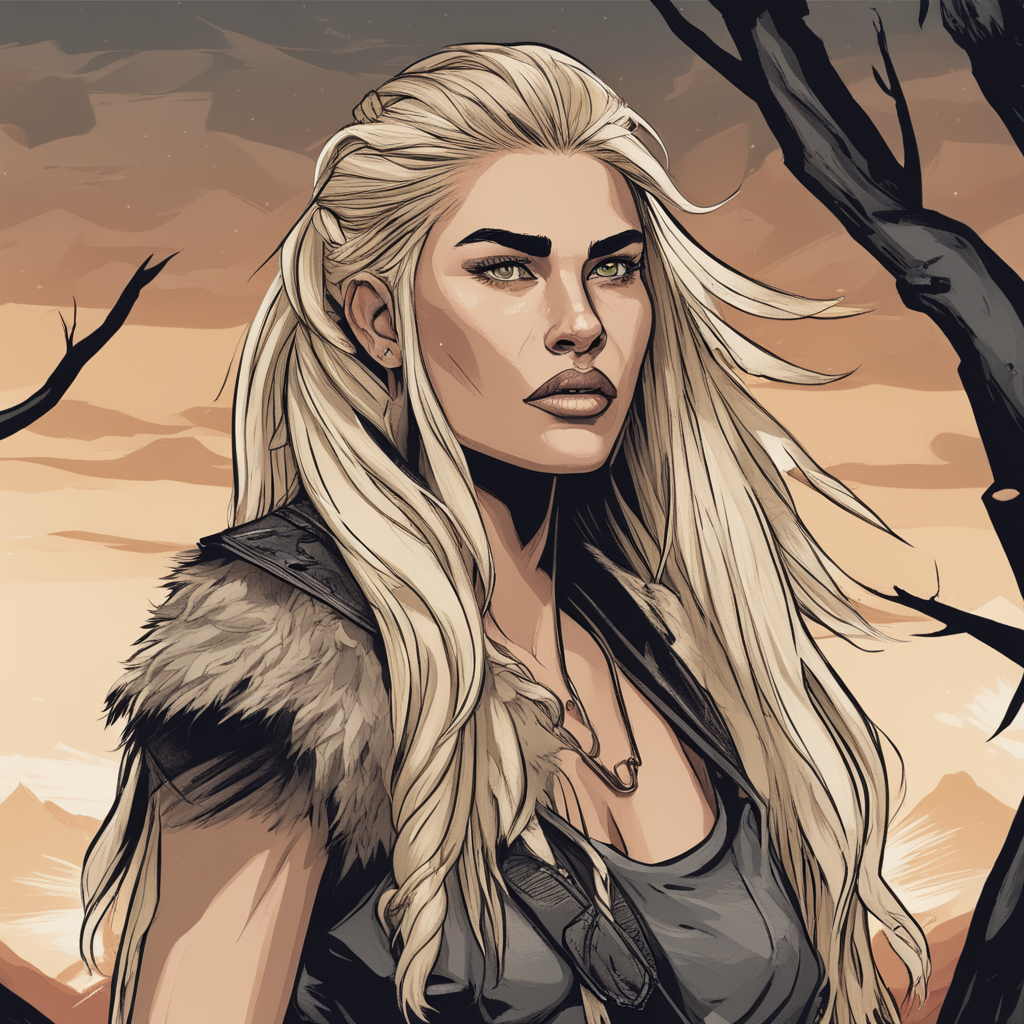
\includegraphics{create-a-digital-illustration-of-branda-a-fierce-and-legendary-woman-with-long-blonde-hair-in-a-hal.png}
\caption{create-a-digital-illustration-of-branda-a-fierce-and-legendary-woman-with-long-blonde-hair-in-a-hal.png}
\end{figure}

Informazioni Generali

Età: 35

Data di nascita: 13/07/1988

Luogo di nascita: Ducatomarrano

Razza: Umana

Classe: Barbara, Via del Totem Guerriero (Lupo della Sila)

Alleati: Gilda dei Guardiani

Nemesi:

Alias: la Fiera


\subsection{Descrizione Generale}\label{descrizione-generale}


\begin{figure}
\centering
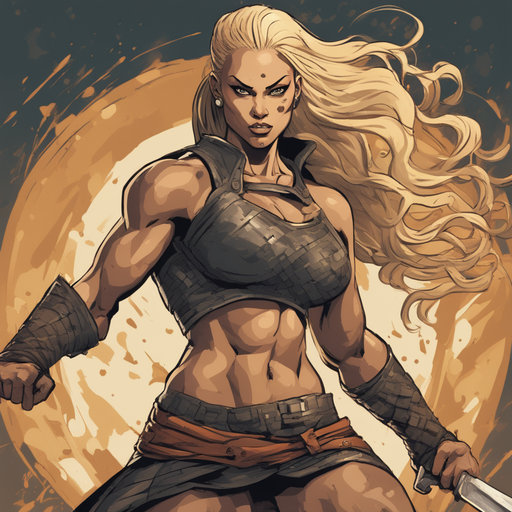
\includegraphics{create-a-digital-illustration-of-branda-a-fierce-and-legendary-woman-with-long-blonde-hair-shaved-o-2.png}
\caption{create-a-digital-illustration-of-branda-a-fierce-and-legendary-woman-with-long-blonde-hair-shaved-o-2.png}
\end{figure}

Branda Gunnarsson, conosciuta come Branda la Fiera, è una figura
leggendaria che si è guadagnata una fama straordinaria Come feroce
avventuriera sempre alla ricerca di avversari più potenti. La sua forza
titanica, la determinazione inarrestabile e l'impegno senza compromessi
nel proteggere la terra l'hanno resa un'icona indiscussa tra gli
avventurieri delle terre selvagge di Valtara.

\subsection{Biografia}\label{biografia}


\subsubsection{Infanzia}\label{infanzia}


Branda la Fiera è nata nel piccolo villaggio di montagna di
Ducatomarrano, circondato da maestose valli e foreste remote. La sua
infanzia è stata segnata da avventure all'aria aperta e da una profonda
connessione con la natura. Fin da piccola, Branda dimostrava una
straordinaria forza fisica e un amore per la vita all'aria aperta. I
suoi genitori, un abile cacciatore e una maestra tessitrice, le hanno
trasmesso preziose abilità di sopravvivenza.

Tuttavia, il destino ha giocato un brutto scherzo quando, all'età di
otto anni, il suo villaggio fu devastato da una terribile inondazione
causata da una violenta tempesta. Questo evento traumatico ha segnato
profondamente Branda e ha risvegliato in lei una determinazione a
proteggere le persone e la natura.

\subsubsection{Adolescenza}\label{adolescenza}


Dopo l'evento dell'inondazione, Branda ha lasciato il suo villaggio
natale in cerca di avventure. Nell'adolescenza, ha viaggiato per
Valtara, esplorando terre sconosciute e affrontando una serie di sfide.
Si è allenata duramente, affinando le sue abilità nel combattimento e
imparando a sopravvivere nelle condizioni più ostili.

Durante questo periodo, ha incontrato e si è alleata con vari
avventurieri, apprendendo da ognuno di loro e guadagnando una
reputazione per il suo coraggio e la sua abilità nel combattimento. Ha
partecipato a missioni per proteggere carovane, sconfiggere mostri e
assistere le comunità in difficoltà.

\subsubsection{Vita Adulta e giorni
nostri}\label{vita-adulta-e-giorni-nostri}


Dopo anni di avventure e crescita personale, Branda ha deciso di
stabilirsi nella pericolosa Foresta dei Giganti in cerca di sfide ancora
più grandi. Questa foresta selvaggia e misteriosa è diventata il suo
nuovo territorio di caccia, dove ha combattuto contro molte delle
creature più feroci e rare del mondo. Qui, ha sviluppato ulteriormente
le sue abilità e ha guadagnato una reputazione tra gli avventurieri come
una forza della natura.

Un giorno, mentre era alla ricerca di un leggendario alce d'argento che
infestava la foresta, ebbe una visione straordinaria di uno spirito lupo
della Sila. Questo incontro divino le rivelò la via della redenzione e
la spinta a mettere le sue abilità al servizio della natura e della
pace. Da allora, Branda ha abbandonato la vita errante per unirsi alla
Gilda dei Guardiani Protettori della Sila e dei Lupi, dedicando la sua
forza e il suo coraggio a proteggere la regione di Valtara e a mantenere
l'ordine tra le creature selvatiche e gli abitanti umani

\subsection{Carriera}\label{carriera}


La carriera di Branda la Fiera è segnata da numerosi combattimenti
eroici e imprese leggendarie. La sua fama come avventuriera la precede,
ed è conosciuta per le sue gesta coraggiose nella Foresta dei Giganti,
dove ha affrontato, da sola, creature temibili come gli orsi delle
caverne giganti, i lupi mannari e si dice persino dei troll.

Dopo la sua conversione alla causa della protezione della natura, Branda
ha continuato a dimostrare la sua dedizione, lavorando con la Gilda dei
Guardiani Protettori della Sila e dei Lupi per preservare gli ecosistemi
di Valtara e mantenere la pace tra le creature selvatiche e gli abitanti
umani. La sua forza, abilità nel combattimento e il suo spirito guida le
hanno permesso di diventare una figura rispettata e una guida per i
giovani aspiranti avventurieri.

\subsection{Personalità}\label{personalituxe0}


Branda è conosciuta per la sua personalità forte e sicura di sé. È prona
all'ira quando è necessario, ma ha imparato a canalizzare la sua rabbia
in modo positivo per combattere le minacce che si presentano. È
appassionata della birra e delle sfide di forza, spesso partecipando a
gare di bevute e gare di sollevamento pesi nei luoghi che visita.

Tuttavia, la sua dedizione alla protezione della natura e la sua
connessione con lo spirito guida del lupo della Sila le conferiscono
anche un lato compassionevole e altruista. È pronta a difendere gli
oppressi e a sacrificare tutto per mantenere l'armonia nella Valtara. La
sua personalità complessa la rende una figura affascinante nel mondo di
D\&D, ammirata sia per la sua forza fisica che per il suo spirito
indomito.


\section{Caravaggio}\label{caravaggio}


\begin{figure}
\centering
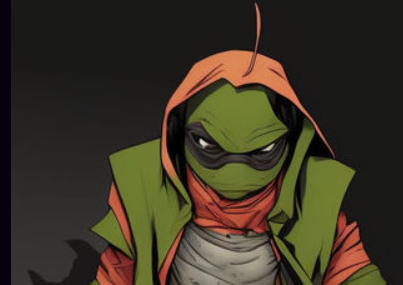
\includegraphics{Screenshot_2023-10-03_204548.png}
\end{figure}

\subsection{Descrizione Generale}\label{descrizione-generale}



Caravaggio è un monaco turtlefolk guerriero. La sua pelle verde scura e
il robusto guscio marrone lo distinguono tra gli altri della sua razza.
Caravaggio è noto per la sua lealtà, il suo coraggio e la sua
determinazione.

\begin{quote}
Citazione {[}location{]}
\end{quote}

\subsection{Biografia}\label{biografia}


Caravaggio è stato adottato da Splinter, un monaco mausefolk, insieme ai
suoi quattro fratelli. Splinter li ha cresciuti e addestrati alle arti
marziali, insegnando loro l'importanza della disciplina e della
protezione degli altri. Durante un viaggio in nave, un tremendo
naufragio ha separato Caravaggio dalla sua famiglia. Ha passato anni a
cercarla, senza mai darsi per vinto, ma non l'ha mai trovata.

\subsection{Carriera}\label{carriera}


Caravaggio ha trovato una nuova casa nelle terre di Valtara, dove ha
messo le sue abilità da combattente a servizio della gilda dei
Protettori. La sua esperienza in combattimento lo ha reso un membro
prezioso dell'organizzazione, impegnato a proteggere la regione dagli
innumerevoli pericoli che la minacciano. Il suo impegno nella gilda è
stato fonte di grande orgoglio, e ha dimostrato di essere un leader
calmo e risoluto quando è necessario.

\subsection{Personalità}\label{personalituxe0}


Caravaggio è noto per la sua lealtà e il suo coraggio. È determinato a
proteggere gli altri dopo aver perso la sua famiglia nel naufragio. Il
principale obiettivo di Caravaggio è riunirsi con i suoi fratelli e con
il suo mentore Splinter. Nel frattempo, si impegna a proteggere Valtara
e le persone che la abitano dai molteplici pericoli che la circondano.
La ricerca dei suoi fratelli è un impegno personale che lo guida in ogni
azione che intraprende.


\section{Disis Iulukinfor}\label{disis-iulukinfor}


\begin{figure}
\centering
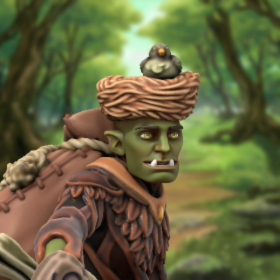
\includegraphics{Disis_Iulukinfor-Token.png}
\caption{Disis Iulukinfor-Token.png}
\end{figure}

Informazioni Generali

Età:

Anno di nascita:

Paese di nascita: Metauros

Razza:

Relazioni:

Alleati:

Nemesi:

Possedimenti importanti:


\subsection{Descrizione Generale}\label{descrizione-generale}


\begin{figure}
\centering
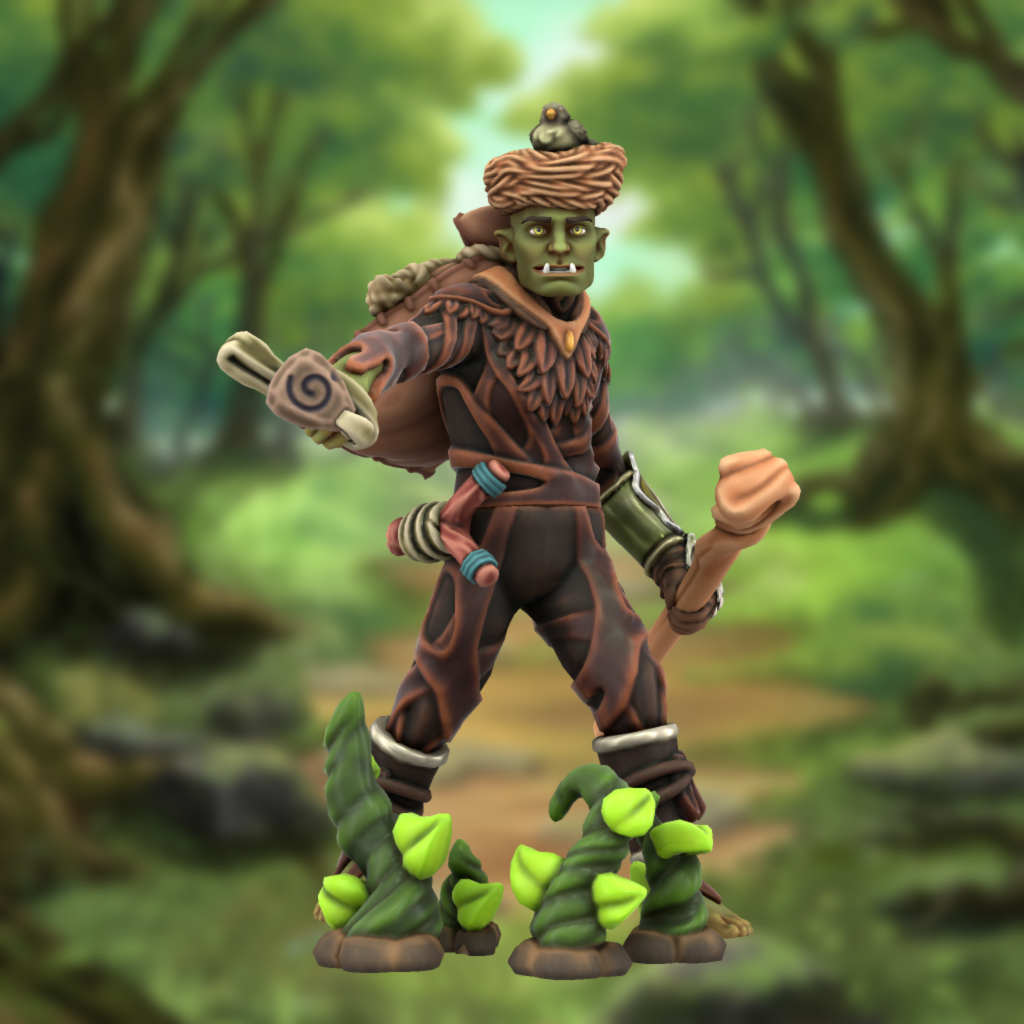
\includegraphics{Disis_Iulukinfor-portrait.png}
\caption{Disis Iulukinfor-portrait.png}
\end{figure}

Disis Iulukinfor è un mezz'orco druido, incarnando l'armonia tra umanità
e natura. La sua pelle abbronzata è attraversata da cicatrici, simboli
del suo passato selvaggio. Gli occhi riflettono saggezza e curiosità,
mentre una chioma corvina incornicia un volto dal fascino unico. Il suo
corpo atletico rivela la profonda connessione con la foresta. Abbigliato
in tonalità terrose, emana un'aura pacifica, trasmettendo sicurezza e un
attaccamento profondo alla natura.

\begin{quote}
``Non sono questi i druidi che state cercando''
\end{quote}

\subsection{Biografia}\label{biografia}


La storia di Disis Iulukinfor inizia con un'origine insolita, nato
dall'incontro tra due mondi, quello umano e quello degli orchi.
Abbandonato poco dopo la nascita nei recessi profondi della foresta,
Disis ebbe la fortuna di essere trovato e adottato dalle creature della
natura. Cresciuto tra animali, spiriti della foresta e creature fatate,
Disis fu avvolto dall'abbraccio amorevole di un ambiente che lo
considerava un proprio figlio. La sua crescita fu segnata
dall'apprendimento dei segreti della natura, dell'arte del druidismo e
della magia che pervadeva gli alberi e le creature stesse. Mentre altri
bambini si familiarizzavano con i confini della società umana, Disis si
immerse nella profonda sapienza delle stagioni, dei venti e degli
animali, diventando un Figlio della Foresta, un protettore e curatore
dell'ambiente che lo aveva accolto. Tuttavia, quando il destino lo portò
a incontrare la civiltà umana, Disis si trovò di fronte a una sfida del
tutto nuova. Confuso e spaesato, si sforzò di adattarsi a usi e costumi
che gli sembravano estranei. La sua capacità di comunicare con gli
animali e il suo cuore gentile gli permisero di stringere amicizie
preziose, aprendo lentamente le porte a un mondo più ampio e complesso.
La sua vita divenne una mescolanza di momenti di contemplazione profonda
nei boschi e di interazioni con le persone che avevano accolto il suo
spirito gentile. Con il tempo, Disis si trasformò in un guardiano della
foresta, un difensore delle creature selvatiche e un portavoce della
natura, cercando di far comprendere agli altri l'importanza di
preservare l'equilibrio dell'ambiente. Liberamente intraprendendo il suo
cammino tra la foresta e le società umane, Disis incarna l'unione di due
mondi e lotta per proteggere l'eredità della foresta che lo ha nutrito,
portando il suo amore per la natura e la sua determinazione a difendere
gli innocenti in ogni angolo del mondo.

\subsection{Carriera}\label{carriera}


La carriera di Disis Iulukinfor non è stata definita da titoli o
posizioni, ma piuttosto da un profondo legame con la natura e il suo
ruolo come guardiano degli equilibri naturali. Fin dalla giovane età,
Disis è stato introdotto alla magia e alla saggezza druidica dalla
foresta stessa. Questa connessione lo ha guidato in un percorso di
apprendimento costante, in cui ha imparato a comunicare con gli animali,
a manipolare le energie naturali e a proteggere l'ambiente circostante.

Inizialmente cresciuto lontano dalla società umana, la sua carriera è
stata forgiata nell'oscurità della foresta, dove ha agito come
intermediario tra le creature selvatiche e gli spiriti della natura. La
sua abilità nel comunicare con gli animali gli ha permesso di sviluppare
un'intesa profonda con le creature che popolano i boschi, facendo di lui
un protettore naturale e un mediatore nei conflitti tra le varie specie.

Con il passare del tempo, il suo ruolo si è espanso, portandolo ad
interagire sempre di più con la società umana. Disis ha iniziato a
condividere la sua conoscenza della natura con coloro che desideravano
ascoltarlo, spiegando l'importanza di rispettare l'ambiente e di
preservare l'equilibrio ecologico. Ha partecipato a iniziative di
conservazione, educando le persone sulle pratiche sostenibili e guidando
escursioni per far conoscere l'ambiente naturale.

La sua carriera non è limitata a un singolo percorso; piuttosto, è un
intreccio di momenti trascorsi nel fitto dei boschi, conversazioni con
creature alate e lezioni impartite su come coesistere in armonia con la
natura. Disis incarna il legame tra l'umanità e il regno naturale,
portando con sé l'eredità del suo passato e la responsabilità del suo
futuro, sempre impegnato a difendere la bellezza e l'equilibrio del
mondo naturale che ama e protegge.

\subsection{Personalità}\label{personalituxe0}


La personalità di Disis Iulukinfor è un intreccio di sfumature,
riflettendo sia l'influenza della natura che la complessità della sua
dualità come mezz'orco. Riservato e riflessivo, Disis porta con sé la
tranquillità dei boschi, un'aura che invita alla contemplazione e al
rispetto. La sua natura tranquilla è un riflesso dell'armonia che cerca
di promuovere nel mondo, facendolo apparire spesso in uno stato di calma
serena.

La sua gentilezza è disarmante, il suo cuore aperto a tutti coloro che
si dimostrano rispettosi e desiderosi di ascoltare le voci della natura.
Con una comunicazione che va al di là delle parole, è in grado di
stabilire connessioni profonde con le creature della foresta, offrendo
amicizia e comprensione dove altri potrebbero vedere solo ferocia.

Sebbene riservato, Disis ha un lato avventuroso e curioso. La sua natura
di Figlio della Foresta lo spinge a esplorare nuovi territori, sia
fisici che emotivi. Questa curiosità lo ha portato a interagire con la
società umana, sfidando le sue ansie e cercando di capire il mondo al di
fuori delle selve.

La sua personalità riflette un profondo rispetto per tutte le forme di
vita. È capace di compassione e di provare dolore per il sofferenza
altrui, ma è altrettanto capace di agire con fermezza quando la natura è
minacciata. La sua determinazione a proteggere l'ambiente naturale e le
creature che vi abitano lo rende un avvocato appassionato per la
conservazione.

In sintesi, Disis è un individuo dalla personalità riflessiva, gentile e
protettiva, ispirato dalla saggezza della natura e determinato a
diffondere armonia e comprensione. La sua personalità è un riflesso del
mondo che abbraccia, un mondo di connessioni profonde e di equilibrio
sottolineato da una passione incrollabile per la conservazione e la
protezione.


\section{Don Tammeo}\label{don-tammeo}


\begin{figure}
\centering
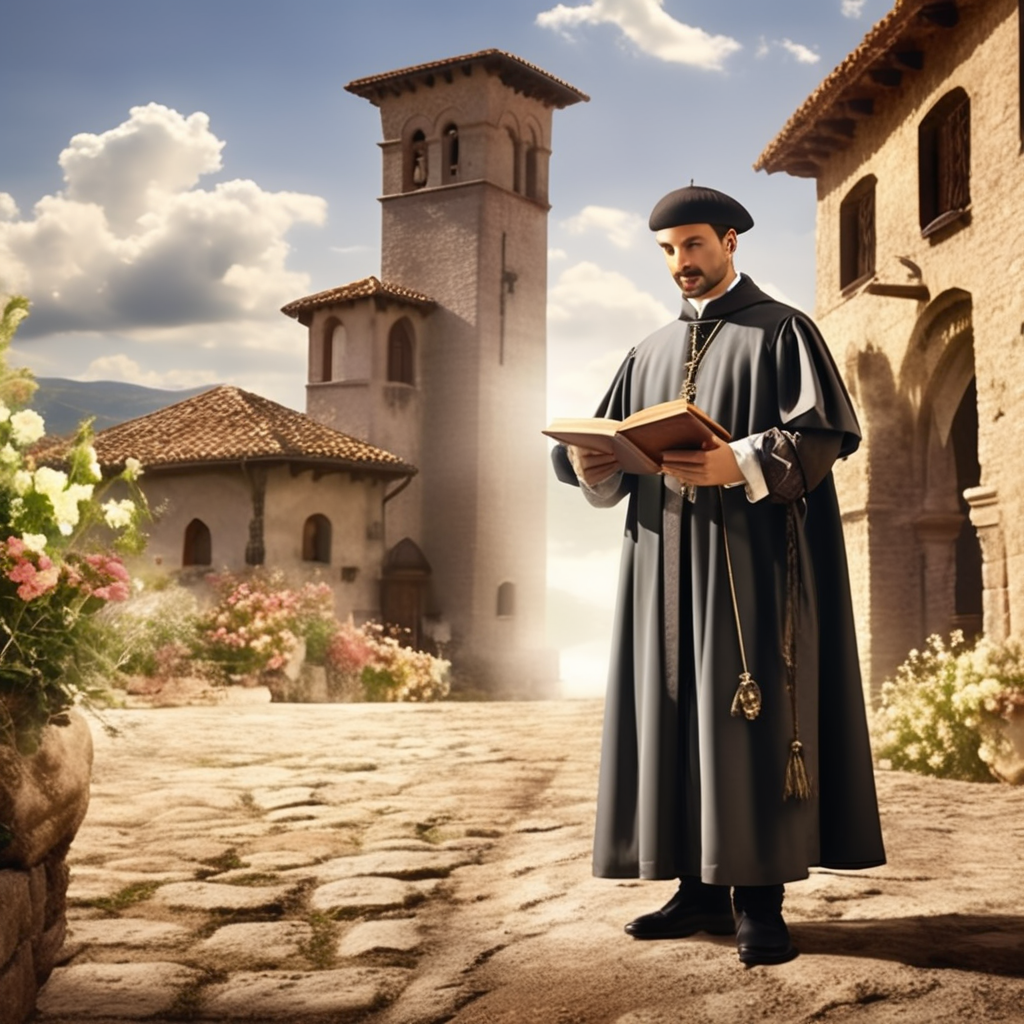
\includegraphics{create-images-of-don-matteo-the-italian-tv-character-in-a-medieval-setting-envision-him-as-a-bene.png}
\end{figure}

\subsection{Descrizione Generale}\label{descrizione-generale}



Don Tammeo è l'incarnazione della speranza nelle strade di Eldrid, un
orfano che ha abbracciato la fede di Luminara Libertas. Membro devoto
della Gilda dei Protettori, la sua presenza irradia compassione e
giustizia, offrendo luce in un mondo avvolto dall'oscurità.

\begin{quote}
``Tutti quanti abbiamo un estremo bisogno di sentirci amati. Ma non c'è
nessuna persona che può colmare questo infinito bisogno d'amore che
abbiamo!'' - Don Tammeo
\end{quote}

\subsection{Biografia}\label{biografia}


\subsubsection{Infanzia}

Don Tammeo è nato sotto il cielo di
\href{Eldrid\%20bd820bb9f6164b39ae6e611a94748518.md}{Eldrid} , ma il
destino gli riservò un percorso diverso. Abbandonato alla sua sorte fin
dalla nascita, Tammeo fu accolto nelle braccia di un orfanotrofio della
città. Crescendo tra i compagni orfani, sviluppò una forza interiore
alimentata dalla necessità di sopravvivere in un mondo spietato.
Tuttavia, durante la sua infanzia, un misterioso evento cambierà il
corso della sua vita. Una notte, mentre osservava il cielo stellato da
una finestra dell'orfanotrofio, ebbe una visione rivelatrice che lo
avvicinò alla fede. Un senso di libertà pervase il suo cuore,
spingendolo a cercare il significato più profondo della vita.

\subsubsection{Adolescenza}

Il richiamo della fede non abbandonò Don Tammeo nemmeno
nell'adolescenza. Spinto dalla visione misteriosa della sua infanzia, si
dedicò agli studi religiosi presso i templi di Eldrid. Con passione e
determinazione, prese i voti e divenne un servo devoto di una divinità
legata al culto della libertà. La sua fede non era solo un insieme di
dogmi, ma una forza guida che plasmò il suo carattere. Tammeo imparò a
condividere il messaggio di speranza e libertà con coloro che
incontrava, diventando una figura di ispirazione per gli altri giovani
che cercavano un significato nella loro esistenza.

\subsubsection{Età Adulta}

Don Tammeo, ora un uomo maturo con il cuore pervaso dalla fede, decise
che la sua missione doveva estendersi oltre le mura del tempio. Sentendo
il richiamo di aiutare coloro che erano in difficoltà, si unì alla Gilda
dei Protettori, un gruppo di individui devoti alla protezione e al
soccorso dei più deboli e bisognosi. La sua dedizione alla giustizia e
la sua connessione con la divinità lo resero un membro rispettato della
gilda. Armato della sua fede incrollabile e della sua compassione per
gli altri, Don Tammeo si adoperò per risolvere i crimini, difendere gli
indifesi e portare la luce della libertà in ogni angolo oscuro di
Eldrid. La sua storia, da orfano a protettore, è diventata una fonte di
ispirazione per la comunità che ha giurato di servire.

\subsection{Carriera}\label{carriera}


Dopo aver preso i voti e aver dedicato la sua vita alla fede di Luminara
Libertas, Don Tammeo ha iniziato il suo cammino come sacerdote
itinerante. Ha viaggiato per Eldrid e le terre circostanti, portando il
messaggio di libertà, speranza e giustizia alle persone che incontrava.
La sua fama di uomo di fede e protettore dei bisognosi ha attirato
l'attenzione della Gilda dei Protettori.

La Gilda, riconoscendo la saggezza e la dedizione di Don Tammeo, lo ha
invitato ad unirsi a loro. Egli ha accettato l'invito, portando la sua
prospettiva unica e il suo zelo per la giustizia all'interno della
gilda. La sua carriera nella Gilda dei Protettori è caratterizzata da
numerosi successi nell'aiutare coloro che sono vittime di ingiustizia e
nell'affrontare minacce criminali.

Don Tammeo ha guadagnato il rispetto dei suoi compagni di gilda e della
comunità di Eldrid, diventando un leader spirituale oltre che un
protettore fisico.

\subsection{Personalità}\label{personalituxe0}


Don Tammeo è un'anima gentile, permeata da una compassione inesauribile.
La sua gentilezza si manifesta attraverso ogni parola e azione, offrendo
conforto a chi è in difficoltà e speranza a coloro che ne hanno bisogno.
La sua fede profonda, ancorata al culto di Luminara Libertas, si traduce
in una determinazione instancabile nel perseguire la libertà e la
giustizia per tutti. Tammeo incarna l'ottimismo, vedendo la luce della
speranza anche nei momenti più bui. La sua integrità morale è come una
guida luminosa, ispirando gli altri a seguire un cammino di rettitudine.
In seno alla Gilda dei Protettori, Don Tammeo assume il ruolo di leader
spirituale, le sue parole fungono da faro guida e il suo impegno per la
causa della libertà crea un legame indissolubile con coloro che
condividono la sua missione. La sua presenza, carica di saggezza e
amore, si staglia come un rifugio sicuro per chi cerca giustizia e
speranza nelle terre di Eldrid


\section{Dorian Be}\label{dorian-be}


\begin{figure}
\centering
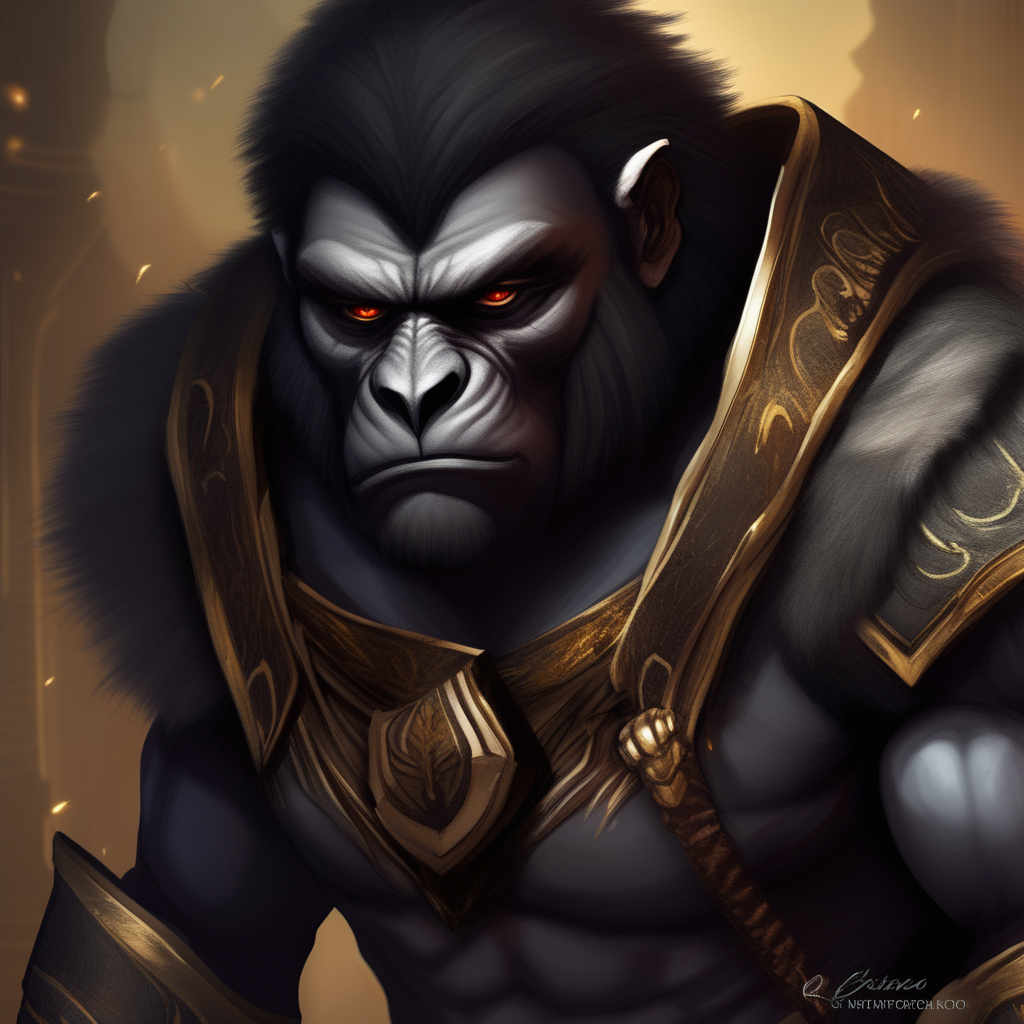
\includegraphics{create-an-image-of-dorian-be-a-heroic-character-from-a-fantasy-world-dorian-is-a-corvilus-a-race---2.png}
\end{figure}

\subsection{Descrizione Generale}\label{descrizione-generale}



Dorian Be è un personaggio di spicco, noto per la sua storia di coraggio
e dedizione nel difendere coloro che sono indifesi. Appartenente alla
misteriosa razza dei Corvilus, che ricorda i gorilla alati, Dorian ha
affrontato tragici eventi che hanno cambiato il corso della sua vita.
Durante la sua carriera circense, condivisa con il suo amato fratello
Haram, ha intrattenuto le folle con spettacoli di giocoleria e abilità
acrobatiche che hanno incantato il pubblico. Tuttavia, una tragedia ha
portato alla perdita delle sue ali e alla morte di Haram, spingendo
Dorian a intraprendere un profondo viaggio di crescita personale. Rinato
come guerriero coraggioso, Dorian ha sviluppato abilità straordinarie
nel combattimento corpo a corpo e la magia arcanica. La sua personalità
compassionevole e protettiva lo ha reso un eroe errante leale, pronto ad
aiutare chiunque abbia bisogno e a portare speranza nei cuori di chi
incontra nel suo cammino.

\begin{quote}
``Tempestate di Like se vi è piaciuta la performance'' - Dorian rivolto
al pubblico
\end{quote}

\subsection{Biografia}\label{biografia}


Dorian Be è nato in un circo itinerante, dove insieme al suo adorato
fratello, Haram Be, intratteneva il pubblico con spettacoli di
giocoleria e abilità acrobatiche. Cresciuto in un ambiente affettuoso e
felice, la loro famiglia circense si considerava una vera e propria
famiglia allargata.

\subsubsection{L'Incidente Tragico}
Un giorno, durante una delle loro esibizioni con bastoni infuocati, un
bambino umano si avventurò inavvertitamente nel perimetro dello
spettacolo. Il fratello di Dorian, Haram, fu distratto dal bambino e
perse il controllo dei bastoni, mettendo in pericolo la vita del
piccolo. Haram, per proteggere il bambino, si lanciò su di lui a
coprirlo, ma fu scambiato per una minaccia e ucciso da una guardia di
paese spaventata.

\subsubsection{La Perdita delle Ali}
Durante la confusione che seguì, Dorian cercò di difendere il corpo
senza vita di Haram, ma fu sopraffatto dalla folla infuriata. Durante la
lotta, subì una profonda ferita sull'ala sinistra da un oggetto
appuntito, rendendo le sue ali irrimediabilmente danneggiate. Incapace
di volare e devastato dalla perdita di suo fratello, Dorian fuggì
portando con sé il corpo del defunto Haram.

\subsubsection{Il Viaggio di Crescita}
Per onorare la memoria di Haram e la loro eredità circense, Dorian
intraprese un lungo viaggio di crescita personale. Cercò maestri saggi e
guerrieri per apprendere le arti del combattimento, della magia e della
forza interiore. Durante il suo viaggio, sviluppò abilità marziali,
apprese a canalizzare l'energia arcana e mantenne vivo il legame con la
natura e le creature alate.

\subsubsection{La Rinascita di Dorian Be}
Dorian Be si trasformò in un combattente agile e coordinato, compensando
la mancanza delle ali con una forza fisica e spirituale incredibile.
Adottò uno stile di vita rispettoso della natura e si impegnò a
proteggere gli esseri vulnerabili, come aveva fatto con il bambino
durante l'incidente che cambiò la sua vita.

\subsubsection{Il Protettore dei Deboli}
Oggi, Dorian Be è noto come un eroe errante, un guerriero
compassionevole che gira il mondo per difendere i deboli, sconfiggere il
male e mantenere vivo lo spirito del circo itinerante che un tempo
condivise con suo fratello Haram. La sua storia toccante e la sua
dedizione nell'assumere la difesa degli oppressi lo hanno reso un
personaggio famoso e rispettato in tutto il mondo di D\&D.

\subsubsection{Eredità di Haram Be}
Dorian Be porta sempre con sé il ricordo del fratello Haram, che
sacrificò la sua vita per proteggere un innocente. Parlando di Haram, i
suoi occhi si illuminano di amore e tristezza, mostrando il legame
indissolubile tra i due fratelli. La memoria di Haram è la forza che
guida Dorian nel suo percorso, e il nome ``Dorian Be'' è diventato un
simbolo di coraggio, protezione e speranza nel mondo di Valtara.

\subsection{Carriera}\label{carriera}


La vita professionale di Dorian può essere divisa in due fasi: la vita
da circense e la vita da guerriero

\subsubsection{Carriera Circense}\label{carriera-circense}

La carriera circense di Dorian Be è iniziata fin da quando era un
giovane gorilla alato. Cresciuto nel cuore di un circo itinerante, ha
imparato sin da piccolo le abilità acrobatiche, la giocoleria e il
carisma necessari per intrattenere il pubblico. Sotto la guida amorevole
dei suoi genitori adottivi e di suo fratello Haram, Dorian si è
trasformato in un abile artista circense, catturando l'attenzione delle
folle con la sua presenza carismatica e le sue abilità impressionanti.
Il duo di fratelli, Dorian e Haram, era la stella del circo, attirando
sempre il pubblico più numeroso. Le loro esibizioni erano spettacolari e
coinvolgenti, con acrobazie mozzafiato e numeri di giocoleria che
sembravano sfidare la gravità stessa. Il legame fraterno tra Dorian e
Haram era evidente sul palco, trasmettendo calore e amore agli
spettatori, che si sentivano parte di una grande famiglia circense.
L'incidente tragico che portò alla morte di Haram e alla perdita delle
ali di Dorian segnò la fine della sua carriera circense. Il circo,
devastato dalla tragedia, continuò senza di loro, ma Dorian sentì di non
poter più esibirsi senza suo fratello. Decise di intraprendere un nuovo
cammino, cercando di onorare la memoria di Haram in altri modi e di
trovare un nuovo scopo nella sua vita.

\subsubsection{Carriera da Guerriero}\label{carriera-da-guerriero}

Dopo aver vissuto un periodo di lutto e riflessione, Dorian Be iniziò il
suo viaggio di crescita personale, intraprendendo una nuova carriera
come guerriero. Sentiva di avere una responsabilità nei confronti della
sua famiglia circense e del ricordo di suo fratello. Decise che doveva
migliorarsi e diventare più forte per poter proteggere coloro che amava
e per difendere gli indifesi da eventuali pericoli. Durante il suo
viaggio, Dorian cercò insegnanti e mentori in diverse arti di
combattimento e magia. Studiò con maestri di arti marziali, imparando a
padroneggiare diverse tecniche di combattimento corpo a corpo. Inoltre,
sviluppò la sua abilità nella magia, scoprendo di poter canalizzare
l'energia arcanica e lanciare incantesimi per difendersi e aiutare gli
altri. Con determinazione e costanza, Dorian affinò le sue abilità,
combinando la forza fisica con la saggezza e la magia. Integrandole con
l'agilità acquisita nella sua carriera circense, Dorian divenne un
guerriero straordinario, capace di fronteggiare nemici e proteggere gli
innocenti. La sua connessione con la natura e le creature alate gli
conferì un legame speciale con gli animali, che spesso lo aiutano nelle
sue missioni. Ha sviluppato una particolare affinità con gli uccelli,
che considera i suoi messaggeri e compagni nell'avventura. Questo legame
speciale gli ha permesso di sviluppare uno stile di combattimento unico,
prendendo ispirazione dai movimenti aggraziati degli uccelli in volo.
Oggi, Dorian Be è un eroe errante, un combattente leale e
compassionevole, con l'abilità di proteggere gli altri con la sua forza
fisica e la magia, mentre mantiene sempre vivo lo spirito del circo
itinerante che una volta condivideva con suo fratello. La sua carriera
da guerriero è diventata una fonte di ispirazione per molti, un esempio
di come il coraggio e la dedizione possano trasformare una tragedia in
un segno di speranza e di difesa per chiunque abbia bisogno di aiuto.

\subsection{Personalità}\label{personalituxe0}


Dorian Be possiede una personalità profondamente empatica e
compassionevole, che è stata plasmata dalle tragedie che ha vissuto. La
perdita di suo fratello Haram ha lasciato un segno indelebile nel suo
cuore, trasformandolo in un individuo protettivo e devoto a coloro che
hanno bisogno di aiuto. È un'anima gentile, sempre pronta a tendere una
mano amica a chiunque sia in difficoltà. Nonostante la sua natura
sensibile, Dorian è anche un individuo coraggioso e tenace. Ha
affrontato numerose sfide e difficoltà nel suo viaggio di crescita,
dimostrando una determinazione inarrestabile nel superarle. La sua
dedizione nel migliorarsi costantemente, sia fisicamente che
mentalmente, lo ha reso un combattente straordinario e un alleato fidato
nei momenti di bisogno. La sua esperienza di circo gli ha donato un
senso dell'umorismo e un lato giocoso, che emergono soprattutto quando è
in compagnia di nuovi amici o quando si trova in situazioni rilassate.
Dorian è sempre pronto a intrattenere il suo gruppo con piccoli trucchi
e acrobazie, portando un po' di leggerezza e divertimento nei momenti
più cupi. Tuttavia, anche se può essere socievole e affabile, Dorian ha
anche dei momenti di intimità e riflessione. I ricordi di suo fratello
Haram possono renderlo triste o nostalgico, ma trova nella sua memoria
la forza per continuare a proteggere e difendere gli altri. La sua
connessione con la natura e le creature alate gli conferisce un profondo
rispetto per l'ambiente circostante e tutte le forme di vita. È un
ambientalista appassionato e cerca sempre di minimizzare l'impatto
negativo che può avere sull'ecosistema, prendendosi cura della fauna e
della flora che lo circondano. Dorian è anche un ascoltatore empatico,
disponibile a dare consigli o conforto quando necessario. Ha imparato
che il potere di proteggere gli altri non si limita solo alla forza
fisica, ma anche a fornire un ascolto attento e un sostegno morale.
Questo atteggiamento compassionevole gli ha guadagnato molte amicizie e
gli ha permesso di formare legami profondi con coloro che incontra nel
suo cammino.


\section{Durso}\label{durso}


\begin{figure}
\centering
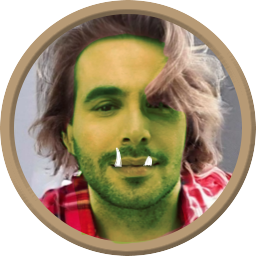
\includegraphics{Durso.png}
\caption{Durso.png}
\end{figure}

Informazioni Generali

Età:

Anno di nascita:

Paese di nascita:

Razza: Mezzorco

Relazioni:

Alleati:

Nemesi:

Possedimenti importanti:


\subsection{Descrizione Generale}\label{descrizione-generale}


\begin{figure}
\centering
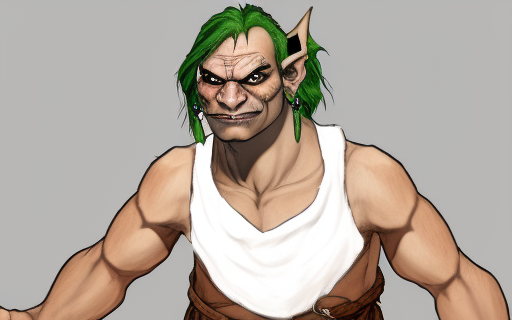
\includegraphics{a-fantasy-orc-that-looks-like-a-male-version-of-barbara-durso-.png}
\caption{a-fantasy-orc-that-looks-like-a-male-version-of-barbara-durso-.png}
\end{figure}

Durso è cresciuto in una tribù di orchi nel cuore della giungla. Fin da
piccolo, si è distinto per la sua stazza imponente e la sua forza
sovrumana. Nonostante l'aspetto minaccioso della sua razza, Durso ha
sempre avuto un cuore buono e un'innata propensione per aiutare gli
altri. Questo lo ha portato spesso a conflitti con gli altri membri
della tribù, che lo consideravano troppo morbido e indulgente.

Un giorno, durante una battuta di caccia, Durso e alcuni compagni della
tribù hanno incontrato un gruppo di avventurieri umani. Durso ha subito
trovato un'affinità con questi stranieri, che non lo giudicavano in base
alla sua razza. Ha iniziato a passare sempre più tempo con loro,
imparando il loro linguaggio e le loro usanze. L'usanza preferita di
Durso era quella nota come ``Postmeridiem V'', secondo la quale tutti si
sedevano attorno ad un fuoco a discutere in maniera semi-seria sui fatti
di cronaca del villaggio.

Con il tempo, Durso ha capito che il suo posto non era nella tribù degli
orchi, ma tra gli avventurieri. Ha lasciato la giungla e si è unito al
gruppo umano, diventando un ciarlatano e uno scaramantico. A volte fa
anche dei riti strani contro la sfortuna, credendo che possano aiutarlo
ad avere successo nelle sue imprese.

La collana di peperoncini che indossa al collo è un talismano che ha
ricevuto da un vecchio sciamano della sua tribù, che gli ha detto che
avrebbe portato fortuna. Durso la porta sempre con sé, convinto che sia
stata la chiave del suo successo come avventuriero.

Nostante la sua parlata un po' rozza, Durso ha un lato più profondo e
riflessivo. Ogni tanto, quando il gruppo si ferma per riposare dopo una
dura avventura, Durso comincia a filosofeggiare e a fare discorsi che
sorprendono i suoi compagni. Proprio come Barbara d'Urso, Durso ha la
capacità di trasformare temi apparentemente banali in riflessioni più
profonde sulla vita e sull'umanità. Anche se a volte i suoi discorsi
possono sembrare un po' strani, i suoi compagni lo rispettano per la sua
saggezza e la sua capacità di vedere le cose da diverse prospettive.

Durso è un buon compagno di squadra e un difensore appassionato dei più
deboli. Anche se non sempre segue le regole, la sua natura caotica buona
lo porta a fare sempre la cosa giusta.

\begin{quote}
``Lei mi sta dicendo che?''
\end{quote}

\subsection{Biografia}\label{biografia}


\begin{figure}
\centering
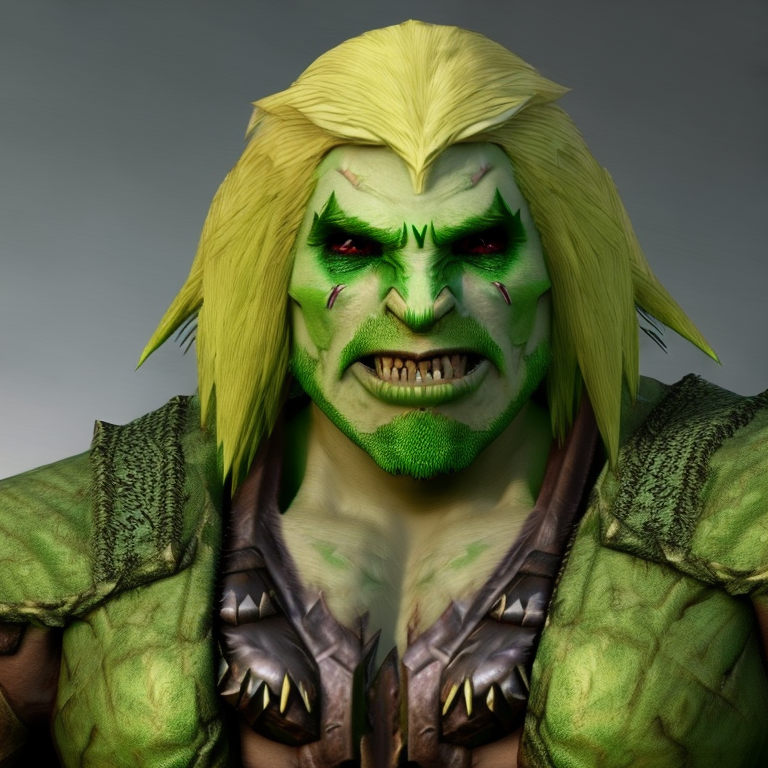
\includegraphics{a-fantasy-orc-that-looks-like-a-male-version-of-barbara-durso-green-skin-blonde-hair--.png}
\caption{a-fantasy-orc-that-looks-like-a-male-version-of-barbara-durso-green-skin-blonde-hair--.png}
\end{figure}

The {[}people group{]} were the region's sole residents prior to the
{[}historical event{]}. {[}New people group{]} arrived in the region
around {[}year{]}.

\subsection{Carriera}\label{carriera}


The history and economic growth of {[}location{]} is tied to
{[}geographic feature{]} which is {[}location's{]} defining
characteristic.

\subsection{Personalità}\label{personalituxe0}



\section{Fabritius Quaterocula (WIP)}\label{fabritius-quaterocula-wip}
\section{Fabritius Quaterocula}\label{fabritius-quaterocula}


\begin{figure}
\centering

\includegraphics{No-Photo-Available-591x591-2.jpg}
\caption{No-Photo-Available-591x591-2.jpg}
\end{figure}

Informazioni Generali

Età: 55

Data di nascita: 9 Maggio 1968

Luogo di nascita: sconosciuto

Razza: Umano

Classe: Guerriero

Alleati:

Nemesi:

Alias:

Professione: Mercenario


\subsection{Descrizione Generale}\label{descrizione-generale}


\begin{figure}
\centering
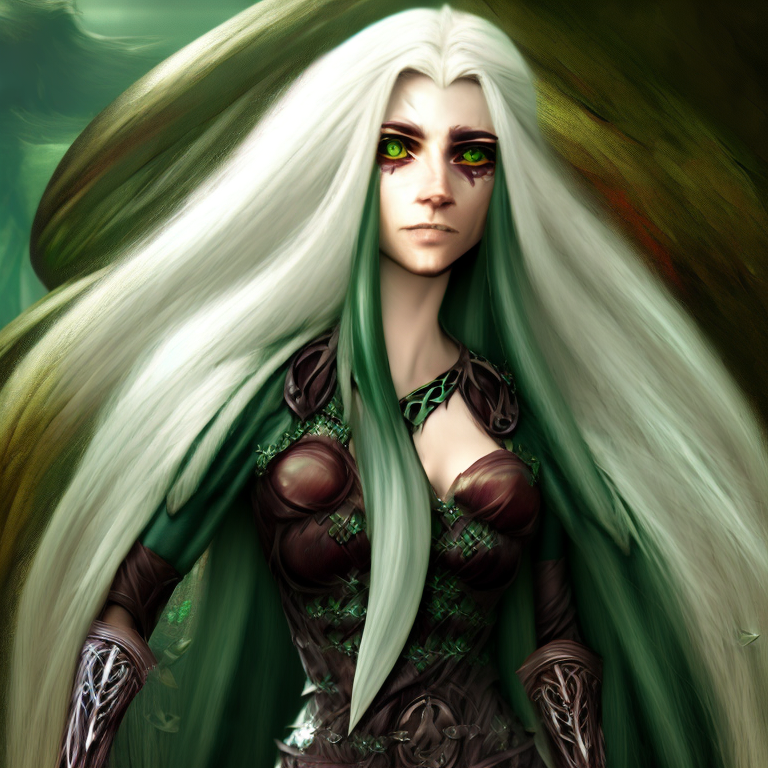
\includegraphics{full-body-portrait-of-a-beautiful-female-elf-with-long-silver-hairs-and-deep-green-eyes-fantasy-se-.png}
\caption{full-body-portrait-of-a-beautiful-female-elf-with-long-silver-hairs-and-deep-green-eyes-fantasy-se-.png}
\end{figure}

Fabritius Quaterocula, conosciuto semplicemente come Fabritius tra gli
ambienti mercenari, è una figura enigmatica e spietata. La sua
reputazione di guerriero senza scrupoli è amplificata dalla sua mancanza
di radici e di un passato noto. La sua avidità è leggendaria, e non
esita a compiere qualsiasi azione, a patto che il prezzo sia adeguato.

\begin{quote}
``Vi faccio vedere come muore un Valtariano'' - Tipico inno di battaglia
di Fabritius
\end{quote}

\subsection{Biografia}\label{biografia}


La vita di Fabritius è avvolta da un velo di mistero. Non ha ricordi
della sua terra natale, né delle sue origini familiari. La sua storia è
una serie di contratti stipulati e denaro guadagnato, senza alcun legame
emotivo che lo lega a un luogo o a una persona. Le storie su di lui sono
spesso accompagnate da sussurri e leggende, alcune delle quali affermano
che abbia venduto la sua anima al diavolo per ottenere il suo spietato
talento bellico, mentre altre sostengono che abbia accumulato così tante
ricchezze da poter comprare qualsiasi cosa, tranne la sua vera identità.

\subsection{Carriera}\label{carriera}


Cresciuto nella scuola della guerra, Fabritius è un maestro di tutte le
armi, un esperto tattico e un assassino spietato quando la situazione lo
richiede. La sua abilità lo rende una presenza temibile e imprevedibile
nei campi di battaglia e tra le ombre delle città. È noto per non fare
domande ai suoi datori di lavoro o sulle loro cause; il suo unico
interesse è il compenso, e ogni contratto rappresenta un'opportunità per
accumulare ulteriori ricchezze. La mancanza di radici e il suo spirito
mercenario fanno sì che Fabritius non conosca alcuna lealtà se non a se
stesso e al suo portafoglio.

\subsection{Personalità}\label{personalituxe0}


Fabritius è un individuo freddo e calcolatore, il cui comportamento è
guidato unicamente dall'avidità e dalla sete di profitto. Nonostante la
sua spietatezza in battaglia, è noto per mantenere un autocontrollo
impeccabile, valutando con attenzione le opportunità che si presentano
per accumulare ricchezza. Non fa domande ai suoi datori di lavoro e
segue gli ordini senza esitazione, a patto che il compenso sia
all'altezza delle sue aspettative.

La sua mancanza di legami emotivi o di un senso di appartenenza a una
comunità lo rende un individuo solitario e privo di scrupoli. Non si fa
scrupoli nel compiere azioni immorali se ciò gli consente di guadagnare
ulteriori monete d'oro. La sua reputazione di individuo imprevedibile e
disposto a tutto per il denaro lo circonda di una sorta di aura di
pericolo.

Fabritius è un individuo isolato, incapace di stabilire relazioni
significative o di instaurare amicizie durature. La sua lealtà è
esclusivamente a se stesso e al suo portafoglio. La sua personalità è
caratterizzata da un pragmatismo senza scrupoli, facendolo agire come un
predatore alla ricerca costante di opportunità per accumulare ricchezze,
indipendentemente dalle conseguenze per gli altri.

\subsection{Coinvolgimenti in Eventi
Recenti}\label{coinvolgimenti-in-eventi-recenti}


\href{Untitled\%20Database\%20cce7df74e0604fb88db6fb1d13af3934.csv}{Untitled
Database}


\section{Gario Miordano}\label{gario-miordano}
\section{Gario Miordano}\label{gario-miordano-1}


\begin{figure}
\centering
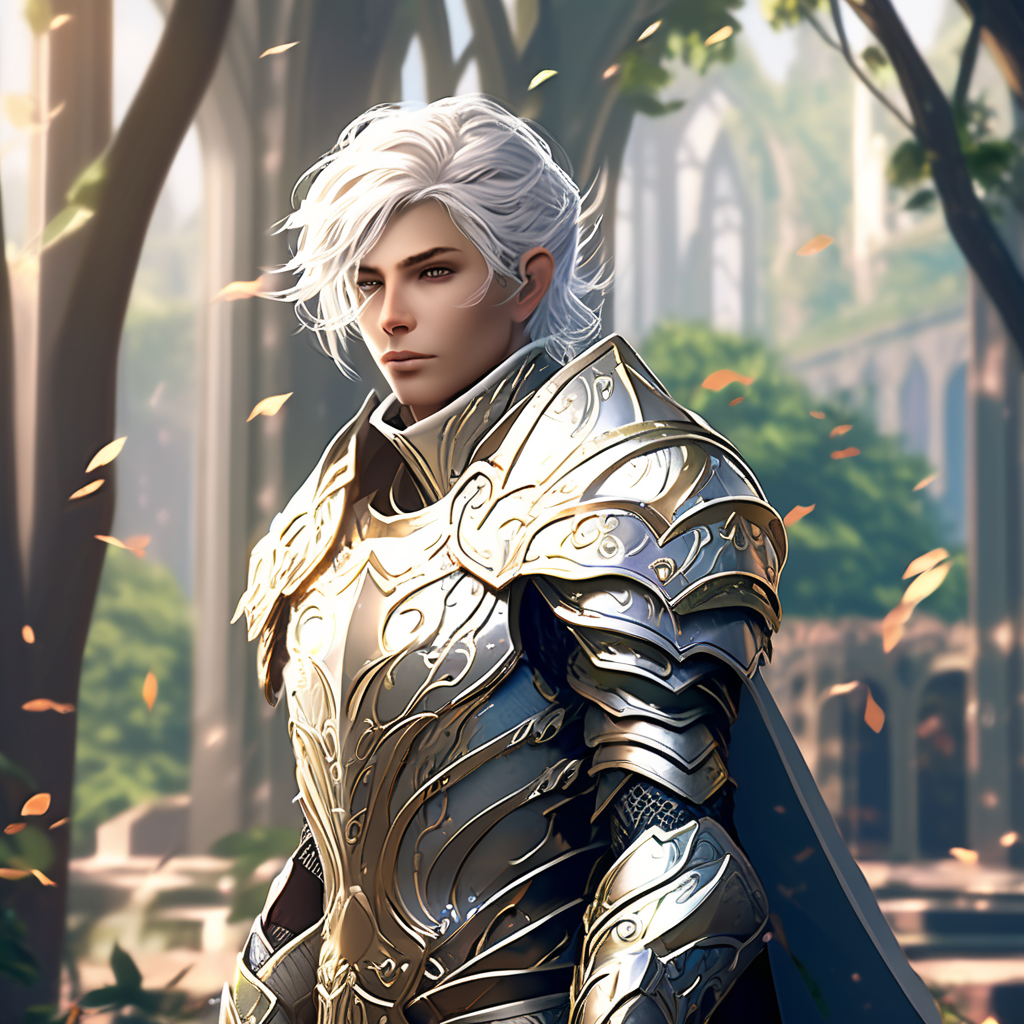
\includegraphics{depict-an-elf-paladin-he-is-a-young-adult-with-short-white-hairs-wearing-full-plate-armour.png}
\caption{depict-an-elf-paladin-he-is-a-young-adult-with-short-white-hairs-wearing-full-plate-armour.png}
\end{figure}

Informazioni Generali

Età: 623

Data di nascita:

Luogo di nascita: Fredo Flu

Razza: Elfo

Classe: Paladino

Alleati:

Nemesi: Le Zucche

Alias:

Professione:


\subsection{Descrizione Generale}\label{descrizione-generale}


\begin{figure}
\centering
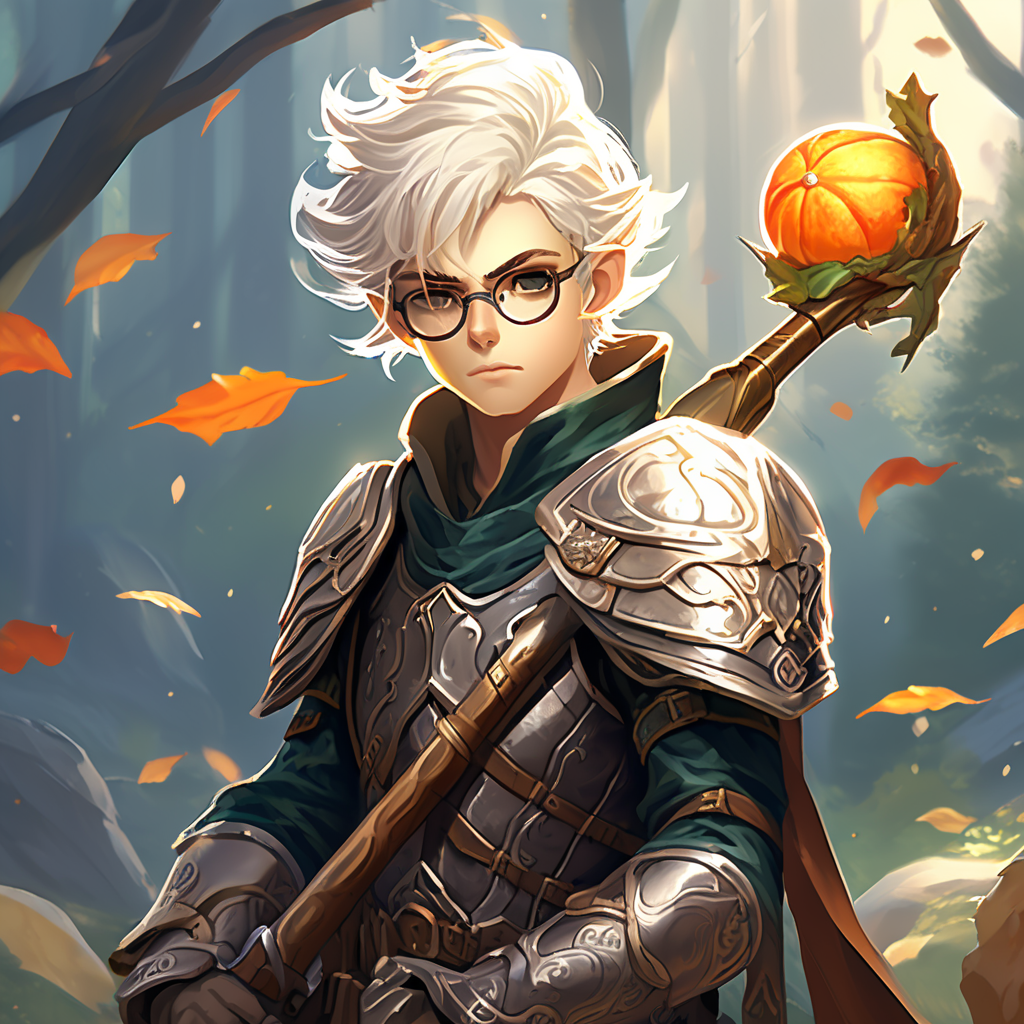
\includegraphics{depict-an-elf-paladin-he-is-a-young-adult-with-short-white-hairs-wearing-full-plate-armour-and-spe-923031639.png}
\caption{depict-an-elf-paladin-he-is-a-young-adult-with-short-white-hairs-wearing-full-plate-armour-and-spe-923031639.png}
\end{figure}

Gario è un elfo paladino di Fredo Flu, con una personalità complessa.
Sebbene animato da un senso di giustizia, è bigotto, xenofobo e
ipocrita, credendo di agire per il bene supremo. Dietro la durezza, ha
un cuore compassionevole, ma le sue azioni spesso suscitano polemiche.

\begin{quote}
``Io le feste di autunno non le voglio festeggiare'' - Gario Miordano
\end{quote}

\subsection{Biografia}\label{biografia}


\subsubsection{\texorpdfstring{\textbf{Origini Nobili e Caduta di
Fredo
Flu}}{Origini Nobili e Caduta di Fredo Flu}}\label{origini-nobili-e-caduta-di-fredo-flu}

Gario Miordano è nato all'interno di una delle più illustri famiglie
elfiche di Fredo Flu, un tempo una delle città più fiorenti e prosperose
del regno elfico. Cresciuto tra l'agio e il lusso, Gario ha goduto di
una vita privilegiata fin dalla sua infanzia, circondato dall'amore e
dall'attenzione della sua famiglia. Tuttavia, la sua vita idilliaca è
stata sconvolta quando una terribile maledizione ha colpito la famiglia
reale di Fredo Flu, causando la sua disfatta e il declino della città.

\subsubsection{\texorpdfstring{\textbf{Fuga a Pandosia e
Coinvolgimento
Politico}}{Fuga a Pandosia e Coinvolgimento Politico}}\label{fuga-a-pandosia-e-coinvolgimento-politico}

Costretto a fuggire insieme alla sua famiglia per sfuggire al destino
che stava per abbattersi su di loro, Gario ha trovato rifugio nella
città di Pandosia, dove è stato accolto da uno dei signori locali.
Durante la sua adolescenza a Pandosia, Gario si è trovato immerso in un
mondo di politica e intrighi, affascinato dalla complessità del potere e
delle relazioni sociali. La sua ambizione lo ha spinto ad avvicinarsi
sempre di più alla scena politica della città, fino a quando non ha
deciso di candidarsi a sindaco.

\subsubsection{\texorpdfstring{\textbf{La Sconfitta e la Profonda
Depressione}}{La Sconfitta e la Profonda Depressione}}\label{la-sconfitta-e-la-profonda-depressione}

Tuttavia, la sua candidatura è stata un fallimento e Gario è stato
sopraffatto da una profonda depressione, incapace di accettare la
sconfitta e il fallimento dei suoi sogni. In preda alla disperazione, ha
abbandonato Pandosia e ha iniziato un lungo viaggio attraverso terre
sconosciute, vagando senza meta per circa cinquant'anni.

\subsubsection{\texorpdfstring{\textbf{Il Giuramento e la Rinascita
Come
Paladino}}{Il Giuramento e la Rinascita Come Paladino}}\label{il-giuramento-e-la-rinascita-come-paladino}

Sulla soglia dei cinquecento anni di età, Gario è giunto in un antico
monastero nascosto tra le montagne, dove ha trovato rifugio e
consolazione. Qui, immerso nella solitudine e nella contemplazione, ha
trovato la fede e ha deciso di prestare giuramento come paladino,
dedicando la sua vita al servizio degli altri e alla difesa dei deboli e
degli oppressi.

\subsubsection{\texorpdfstring{\textbf{La Leggenda dello
Spaccazzucca}}{La Leggenda dello Spaccazzucca}}\label{la-leggenda-dello-spaccazzucca}

Durante i suoi vagabondaggi, Gario si trovò ad affrontare una minaccia
inaspettata: una banda di briganti malvagi che aveva preso d'assalto un
villaggio agricolo. Questi briganti, noti per la loro crudeltà, avevano
preso il controllo del villaggio e avevano iniziato a saccheggiare le
colture di zucche, essenziali per la sopravvivenza della comunità.
Gario, mosso dalla compassione per gli abitanti del villaggio e
determinato a porre fine alla tirannia dei briganti, affrontò i
malviventi con coraggio e astuzia.

Durante la battaglia che ne seguì, Gario afferrò una grande mazza di
legno e la usò con grande maestria contro i suoi avversari. Con ogni
colpo, le zucche che i briganti avevano rubato dal villaggio si
frantumavano sotto la forza travolgente della mazza di Gario. Il suono
sordo degli schianti delle zucche riempiva l'aria mentre Gario
combatteva con ferocia e determinazione. Alla fine, grazie alla sua
abilità nel combattimento e alla sua astuzia, Gario riuscì a sconfiggere
i briganti e a restituire la pace e la sicurezza al villaggio. Da quel
giorno in poi, Gario fu conosciuto come ``Lo Spaccazzucca'', in onore
della sua impresa eroica che aveva visto le zucche rotolare sotto la sua
mazza come se fossero state fatte di vetro.

\subsection{Carriera}\label{carriera}


\subsubsection{Carriera Politica}\label{carriera-politica}

Durante il periodo trascorso a Pandosia, Gario Miordano si immerse
attivamente nella politica locale, attratto dalla complessità dei giochi
di potere e dalle dinamiche sociali della città. Pur non essendo ancora
direttamente coinvolto nella politica ufficiale, Gario partecipò
attivamente alle discussioni comunitarie e alle riunioni pubbliche,
esprimendo le sue opinioni su questioni di interesse cittadino e
sostenendo cause che riteneva giuste e importanti. La sua voce risuonava
con autorità e rispetto tra i suoi concittadini, che apprezzavano la sua
sincerità e la sua dedizione alla causa del bene comune. Questa
esperienza lo ha preparato per la sua futura carriera politica,
fornendogli le basi necessarie per affrontare le sfide e le
responsabilità che avrebbe incontrato nel corso della sua vita pubblica.

\subsubsection{\texorpdfstring{\textbf{Carriera Come
Paladino}}{Carriera Come Paladino}}\label{carriera-come-paladino}

Dopo aver giurato fedeltà al monastero e aver abbracciato la vita da
paladino, Gario Miordano ha dedicato ogni istante della sua esistenza
alla difesa dei deboli e alla lotta contro le forze del male. Grazie
alla sua abilità nel combattimento e alla sua fede incrollabile, ha
affrontato numerosi nemici, da orde di creature oscure a potenti maghi
oscuri, dimostrando sempre una straordinaria determinazione e coraggio.
La sua reputazione di paladino valoroso e intraprendente si è diffusa
rapidamente, guadagnandogli il rispetto e l'ammirazione di coloro che
hanno avuto la fortuna di combattere al suo fianco. Attraverso le sue
imprese eroiche e il suo impegno costante per la giustizia e la
rettitudine, Gario continua a incarnare gli ideali dei Protettori,
servendo come esempio luminoso di sacrificio e dedizione per tutti
coloro che lo incontrano.

\subsection{Personalità}\label{personalituxe0}


Gario Miordano è caratterizzato da un atteggiamento bigotto, xenofobo e
ipocrita, sebbene sia convinto di agire per il bene supremo. La sua
rigida interpretazione delle sue credenze e la sua mancanza di
tolleranza nei confronti di chi è diverso da lui lo portano spesso a
manifestare pregiudizi e discriminazioni verso altre razze e culture.
Pur professando di difendere gli ideali di giustizia e moralità, Gario
mostra spesso un duplice standard nel trattare gli altri, giudicando
severamente i peccati altrui mentre giustifica i suoi stessi
comportamenti discutibili. La sua ipocrisia emerge quando, nonostante le
sue azioni discriminatorie, crede fermamente di essere dalla parte della
rettitudine e della verità. In certi momenti, Gario può dimostrare
generosità e compassione, ma spesso queste qualità sono riservate solo a
coloro che condividono le sue stesse convinzioni, mentre gli altri
vengono trattati con disprezzo e ostilità. In definitiva, la personalità
di Gario Miordano è contraddistinta da una complessa intersezione di
bigottismo, xenofobia e ipocrisia, che lo rende un individuo controverso
e difficile da comprendere.


\section{Gnomio Cartonio}\label{gnomio-cartonio}


\begin{figure}
\centering
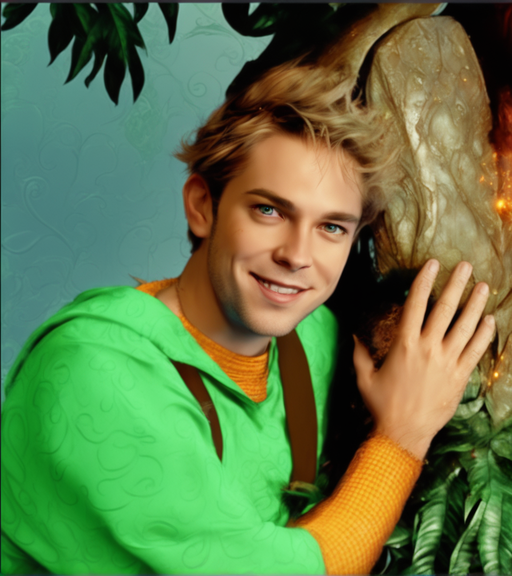
\includegraphics{gnomo-epic-royal-background-big-royal-uncropped-crown-royal-jewelry-robotic-nature-full-shot-.png}
\end{figure}

\subsection{Descrizione Generale}\label{descrizione-generale}



Gnomio è uno gnomo giovane e intraprendente che vive nel tranquillo
Fantabosco, un affascinante villaggio gnomico situato nella Valtara
Meridionale, al confine con il Regno degli Alisei. Sin da bambino, ha
sognato di diventare uno dei più grandi eroi di Fantabosco e ha un
desiderio ardente: uccidere un drago e creare un'armatura di scaglie di
drago che diventi leggendaria a Valtara. La sua vita è un'avventura in
continua evoluzione, guidata dalla passione per la storia dei draghi e
il desiderio di gloria.

\begin{quote}
``Che testa di pigna che sono!''
\end{quote}

\subsection{Biografia}\label{biografia}


Gnomio è nato a Fantabosco da una famiglia di gnomi con una lunga
tradizione di artigianato. Fin dall'infanzia, è stato affascinato dalle
storie dei draghi raccontate dai viaggiatori che passavano per il suo
villaggio. La madre di Gnomio, Mamma Antelitteram, è stata una figura
determinante nella sua vita, spingendolo ad avvicinarsi alla Gilda dei
Protettori per poter garantire il suo sostentamento. Questo è stato un
passo cruciale che ha influenzato la sua carriera.

\subsection{Carriera}\label{carriera}


La passione di Gnomio per la storia dei draghi lo ha spinto a diventare
un abile archeologo, dedicando innumerevoli ore a scavare tra le rovine
antiche e a esaminare manufatti per apprendere tutto ciò che poteva. Da
adulto, ha deciso di diventare un ranger specializzato nella caccia alle
creature magiche, in particolare ai draghi. Ha perfezionato le sue
abilità di combattimento, apprendendo a sopravvivere nella natura
selvaggia e ad affrontare i pericoli della Foresta dei Giganti.

Il suo percorso lo ha portato a viaggiare in luoghi remoti alla ricerca
di indizi sulle possibili dimore dei draghi. L'affiliazione alla Gilda
dei Protettori è stata inizialmente una scelta dettata dalla necessità
finanziaria, ma ha presto compreso che questa opportunità gli avrebbe
permesso di perseguire la sua passione in modo più completo.

\subsection{Personalità}\label{personalituxe0}


Gnomio è noto per la sua determinazione e la sua curiosità insaziabile.
È un individuo tenace, sempre in cerca di nuove conoscenze e disposto a
mettere alla prova se stesso per raggiungere i suoi obiettivi. Tuttavia,
è anche affettuoso e legato alla sua amata Fata Ficarella, che lo ispira
costantemente e gli dà la motivazione per cercare la gloria.

Porta sempre con sé una fiaschetta di cuoio contenente la Scivolizia,
una bevanda tipica del suo villaggio. Questa bevanda particolare è un
segno tangibile delle sue radici e delle sue origini a Fantabosco, ed è
un ricordo costante della sua madre e del suo villaggio natale. Gnomio è
dunque un personaggio con un equilibrio tra la determinazione e
l'attaccamento alle proprie radici, pronto a intraprendere audaci
avventure per realizzare il suo sogno di diventare un eroe leggendario
di Valtara.


\section{Grunt Martelcuore}\label{grunt-martelcuore}


\begin{figure}
\centering
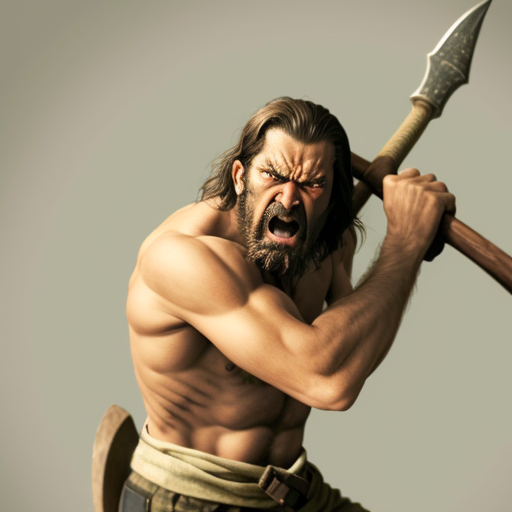
\includegraphics{an-angry-man-with-a-double-axe.png}
\end{figure}

\subsection{Descrizione Generale}\label{descrizione-generale}


Grunt è un nano robusto e massiccio, con mani grosse e callose,
testimonianza dei lunghi anni trascorsi a lavorare con materiali grezzi
nelle montagne. Indossa abiti robusti e pratici, preferendo pelli e
tessuti resistenti per sopportare le dure condizioni del mondo esterno.
Sulla schiena porta una ascia bipenne, sua arma preferita.

\begin{quote}
``Tu! Dammi altro cibo!''
\end{quote}

\subsection{Biografia}\label{biografia}


Grunt è nato e cresciuto tra le montagne a sud di Azura, con la tribù
dei Martelcuore, un gruppo di nani che ha sempre disdegnato la civiltà.
La sua infanzia è stata segnata da giorni trascorsi nelle grotte e nelle
valli nascoste tra montagne, imparando a sopravvivere grazie a un
profondo legame con la natura circostante. Grunt ha sviluppato una forza
brutale che lo ha fatto risaltare tra i suoi simili.

\subsection{Carriera}\label{carriera}


Un incontro casuale con un gruppo di avventurieri provenienti dalla
Gilda dei Protettori di Azura ha cambiato la vita di Grunt. La sua
incredibile abilità nel combattimento e la sua capacità naturale di
sopravvivenza lo hanno reso un membro apprezzato della gilda. Grunt ha
abbandonato la vita nelle montagne per unirsi alla Gilda dei Protettori
di Azura, aprendo così le porte alla scoperta di nuove terre e
avventure. Combattendo per la gilda, Grunt ha dimostrato di essere un
alleato valoroso, anche se la sua scarsa conoscenza delle città e delle
leggi lo porta spesso in situazioni comiche.

\subsection{Personalità}\label{personalituxe0}

Grunt è noto per la sua lealtà e per il suo stomaco senza fondo. La sua
natura barbarica si combina con una curiosità ingenua nei confronti
della civiltà, portandolo a imparare lentamente le stranezze della vita
in città. È un combattente determinato, pronto a proteggere i suoi
alleati con la sua forza brutale. La sua semplicità e il suo spirito
libero possono portare a momenti di comicità e imbarazzo, ma la sua
genuinità lo rende un amico fidato e un compagno di avventura pronto a
tutto, soprattutto quando viene ricompensato con un lauto pasto. Grunt è
ansioso di esplorare il mondo al di fuori delle montagne e sta appena
iniziando la sua avventura.



\section{Hartley}\label{hartley}


\begin{figure}
\centering
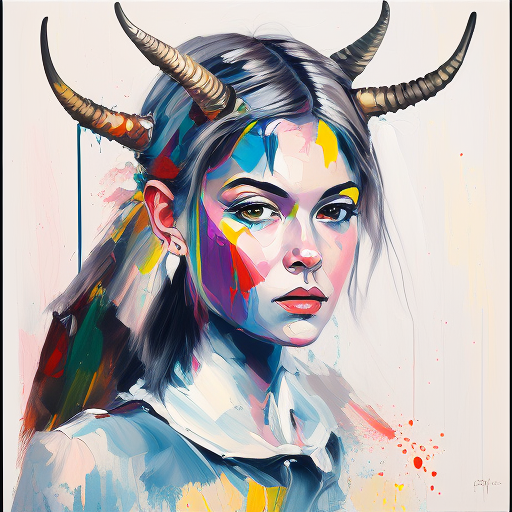
\includegraphics{Hartley_autoritratto.png}
\caption{Hartley\_autoritratto.png}
\end{figure}

Informazioni Generali

Età: 25

Anno di nascita: 1998

Paese di nascita: Kos

Razza: Tiefling

Relazioni:

Alleati:

Nemesi:

Possedimenti importanti:


\subsection{Descrizione Generale}\label{descrizione-generale}


\begin{figure}
\centering
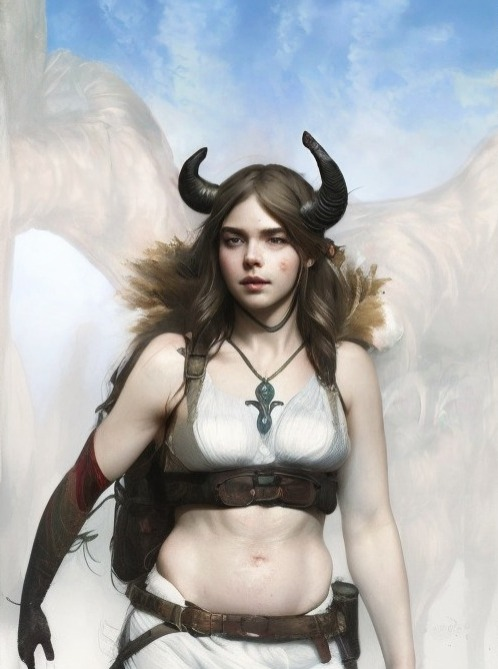
\includegraphics{Hartley.jpeg}
\caption{Hartley.jpeg}
\end{figure}

Lettera di risposta di Marpalo (Quartiermastro dei Protettori di Kos)
alla richiesta di Sitahu di inviare ad Azura un protettore adatto ad una
missione di spionaggio.

``Come mi hai chiesto, ecco tutto quello che so su Hartley Nessuno
conosce la sua vera storia, perché racconta una cosa diversa ogni volta
che qualcuno gliela chiede. A volte è scappata dall'estremo Nord a causa
delle persecuzioni contro i tiefling, altre volte è un'ex prostituta che
ha dovuto uccidere il suo pappone per conquistare la propria libertà,
altre ancora una principessa scappata dal massacro della sua famiglia
durante le rivolte popolari di chissà quale regno lontano. Non
conosciamo neanche il suo cognome, in tasca ha sempre più di un
documento pronto a testimoniare in favore delle sue molteplici
personalità. Probabilmente neanche lei si ricorda più come si chiama.
Bugiarda patologica, ma convincente, mente anche quando non c'è alcun
motivo valido per farlo. Il problema più grande è il suo modo di fare:
sempre cordiale, di buon umore, pronta ad ascoltare e a compatire.
Diresti di lei che è la tua amica più fidata, almeno fino a quando non
riesce ad ottenere da te quello di cui aveva bisogno. Di lei sappiamo
solo che si guadagnava da vivere per strada, distraendo i passanti con
giochi di prestigio e derubandoli mentre lo faceva. Alla fine dello
spettacolo le lasciavano anche qualche monetina (se non le aveva già
prese)! Col passare del tempo ha alzato il tiro, arrivando a svaligiare
le case e gli appartamenti dei cittadini più ambienti della città, fino
a quando non ha fatto il passo più lungo della gamba. Ha deciso di
introdursi nella casa di noto politico Kosentino, uno degli uomini più
influenti di Kos, con una delle case più sorvegliate della città. È
riuscita ad entrare senza fatica, e di questo le bisogna dare merito, ma
non è più uscita. Dopo essere stata catturata avrebbe potuto finire il
resto dei suoi giorni in galera, ma per sua fortuna il suo bersaglio è
anche uno dei principali benefattori della Gilda dei Protettori, e le ha
proposto di mettere le sue capacità al servizio dei bisognosi, lavorando
per la Gilda. In cambio avrebbe fatto decadere tutte le accuse che
gravavano sulla sua testa. Ancora ci chiediamo come sia possibile che le
abbia concesso una grazia del genere, probabilmente è caduto vittima dei
suoi incantesimi da manipolatrice! È stata scortata alla Gilda dalle
guardie cittadine, che hanno presidiato la nostra sede per poco più di
una settimana, poi sono sparite. Hartley da allora è con noi, anche se
adesso potrebbe scappare con il nostro equipaggiamento e spacciarsi per
una Protettrice. Si è rivelata un'ottima risorsa in più di una missione,
riesce ad a trovare una soluzione anche nelle situazioni più difficili,
e non c'è serratura che riesca a fermarla. Tuttavia si rifiuta di
combattere, non si abbassa a ``barbarie del genere'', come dice spesso.
``Le giuste parole aprono più teste di una scure'' dice anche. Spero che
queste informazioni ti possano essere utili nella scelta dei componenti
per la tua squadra. Porta i miei saluti alla tua Francine e ai piccoli
Tuo Marpalo''


\subsection{Coinvolgimenti in eventi
recenti}\label{coinvolgimenti-in-eventi-recenti}


\href{Untitled\%20Database\%20f0a0837cffd44ac7a9471133f60c97b8.csv}{Untitled
Database}

\subsection{6. Scheda personaggio}\label{scheda-personaggio}


\href{Info\%20PG\%20792973e9c98e424b8fa1da3d1c2eeac4.csv}{Info PG}

\subsubsection{Statistiche e abilità}\label{statistiche-e-abilituxe0}


\href{Abilita\%CC\%80\%207db3a6b653ad434187ea54a65d788929.csv}{Abilità}

\subsubsection{Lista magie}\label{lista-magie}


\section{Ken Nataro}\label{ken-nataro}
\section{Ken Nataro}\label{ken-nataro-1}


\begin{figure}
\centering
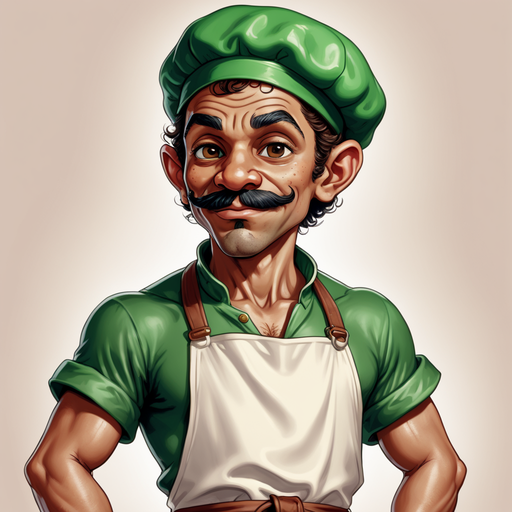
\includegraphics{create-a-digital-illustration-of-ken-nataro-a-mulatto-skinned-halfling-with-a-sturdy-physique-ken--7.png}
\caption{create-a-digital-illustration-of-ken-nataro-a-mulatto-skinned-halfling-with-a-sturdy-physique-ken--7.png}
\end{figure}

Informazioni Generali

Età: 59

Data di nascita: 20/04/1964

Luogo di nascita: Kos

Razza: Halfling

Relazioni: Sposato con Balorca

Alleati: Gilda dei protettori

Alias: U furnaru

Professione: Panettiere


\subsection{Descrizione Generale}\label{descrizione-generale}


\begin{figure}
\centering
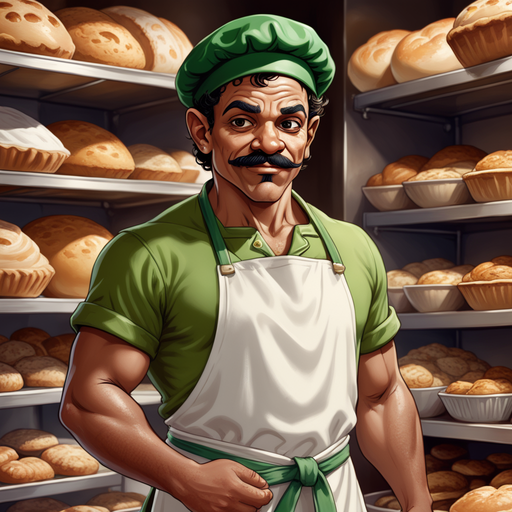
\includegraphics{create-a-digital-illustration-of-ken-nataro-a-mulatto-skinned-halfling-with-a-sturdy-physique-ken--9.png}
\caption{create-a-digital-illustration-of-ken-nataro-a-mulatto-skinned-halfling-with-a-sturdy-physique-ken--9.png}
\end{figure}

Ken Nataro è un halfling di anni con un aspetto insolito per la sua
razza. È dotato di potenti braccia muscolose, frutto di anni e anni di
duro lavoro nella sua panetteria ``da Nataro''. La sua pelle è
abbronzata dal sole e il suo viso mostra rughe di esperienza e di vita
vissuta. I suoi occhi sono vivaci e riflettono la profonda ira che
cresce in lui quando si trova di fronte all'ingiustizia.

\subsection{Biografia}\label{biografia}


\subsubsection{Infanzia}\label{infanzia}

Ken Nataro è nato in una famiglia di panettieri halfling con una
tradizione secolare di produzione del pane. Fin da piccolo, Ken mostrava
un interesse vivace per il mestiere di famiglia. Mentre i suoi coetanei
giocavano a nascondino, Ken preferiva impastare la pasta e osservare il
pane lievitare nel forno a legna. La panetteria ``da Nataro'' era il
cuore pulsante della comunità halfling di Kos, e Ken amava passare il
tempo con i suoi genitori e i suoi nonni mentre apprendeva i segreti
dell'arte della panificazione.

\subsubsection{\texorpdfstring{\textbf{Eredità della
Panetteria}}{Eredità della Panetteria}}\label{eredituxe0-della-panetteria}

All'età di anni, dopo anni di apprendistato e duro lavoro nella
panetteria di famiglia, Ken ereditò ufficialmente la gestione della
panetteria ``da Nataro'' dai suoi genitori. Questo fu un momento di
grande responsabilità, ma anche di orgoglio per Ken, che si sentiva
onorato nel portare avanti la tradizione familiare. La panetteria era
famosa in tutta Kos per il suo pane fragrante e le sue prelibatezze da
forno, che erano richieste persino dai nobili di Kos durante le
festività.

\subsubsection{\texorpdfstring{\textbf{La Lenta
Decadenza}}{La Lenta Decadenza}}\label{la-lenta-decadenza}

Nonostante il suo impegno instancabile e il desiderio di preservare la
gloria della panetteria, Ken dovette affrontare tempi difficili. I
cambiamenti nel commercio del grano e le fluttuazioni economiche in Kos
iniziarono a colpire la sua attività. La panetteria ``da Nataro'' non
era più la potenza economica di un tempo, e Ken faticava a mantenere i
livelli di produzione e a sbarcare il lunario. Questi tempi difficili
fecero emergere in lui la sua innata ira e desiderio di ristabilire
l'equilibrio nella sua vita.

\subsubsection{\texorpdfstring{Entrata ne\textbf{lla Gilda dei
Protettori}}{Entrata nella Gilda dei Protettori}}\label{entrata-nella-gilda-dei-protettori}

Per affrontare le crescenti difficoltà finanziarie e sostenere la sua
numerosa famiglia, Ken prese una decisione radicale. All'età di anni,
lasciò la gestione quotidiana della panetteria nelle mani di sua moglie,
Balorca, una mezz'orca dal cuore gentile, e decise di unirsi alla Gilda
dei Protettori. Questa decisione fu dettata dalla necessità di
guadagnare un reddito extra, ma anche dalla sua crescente ira per le
ingiustizie del mondo. Ken trasformò la sua rabbia in una forza
formidabile nel campo di battaglia, diventando un membro valoroso della
gilda. Oggi, Ken Nataro bilancia la sua vita da panettiere con le sue
nuove avventure come barbaro nella Gilda dei Protettori. La sua
dedizione alla sua famiglia, la sua passione per la panificazione e il
suo desiderio di giustizia sono i pilastri della sua vita, rendendolo un
personaggio complesso e affascinante nel mondo di Kos.

\subsection{Personalità}\label{personalituxe0}


Ken Nataro è un individuo di straordinaria forza d'animo e
determinazione. La sua personalità è caratterizzata da un profondo senso
di responsabilità e un attaccamento radicato alla sua famiglia e alla
sua tradizione. È gentile e affettuoso con i suoi dieci figli, e la sua
relazione con sua moglie, Balorca, è fondata su un amore profondo e una
profonda comprensione reciproca.

Tuttavia, sotto la superficie calma e affettuosa, alberga una fiamma di
ira ardente. Le ingiustizie del mondo, in particolare quelle che hanno
colpito la sua amata panetteria di famiglia, alimentano la sua
determinazione a fare del bene e a ristabilire l'equilibrio. Quando si
trova di fronte all'ingiustizia o alla crudeltà, questa ira si trasforma
in una forza indomabile che lo guida in battaglia, conferendo a Ken un
coraggio straordinario e una capacità di combattimento formidabile.

Ken è anche noto per la sua generosità e la sua propensione a sostenere
chi è in difficoltà, e questo lo rende un membro prezioso della Gilda
dei Protettori. È sempre pronto a tendere una mano agli amici e agli
alleati e a difendere coloro che non possono difendersi da soli. La sua
personalità complessa, con una mescolanza di gentilezza, ira e spirito
combattivo, lo rende un personaggio affascinante e un alleato fidato
nelle avventure di Kos

\subsection{Coinvolgimenti in eventi
recenti}\label{coinvolgimenti-in-eventi-recenti}


\href{Untitled\%206d32341cd290432098378da8e9e19b98.csv}{}


\section{Kit (WIP)}\label{kit-wip}


\begin{figure}
\centering

\includegraphics{No-Photo-Available-591x591-2.jpg}
\caption{No-Photo-Available-591x591-2.jpg}
\end{figure}

Informazioni Generali

Età:

Anno di nascita:

Paese di nascita:

Razza:

Relazioni:

Alleati:

Nemesi:

Possedimenti importanti:


\subsection{Descrizione Generale}\label{descrizione-generale}


\begin{figure}
\centering
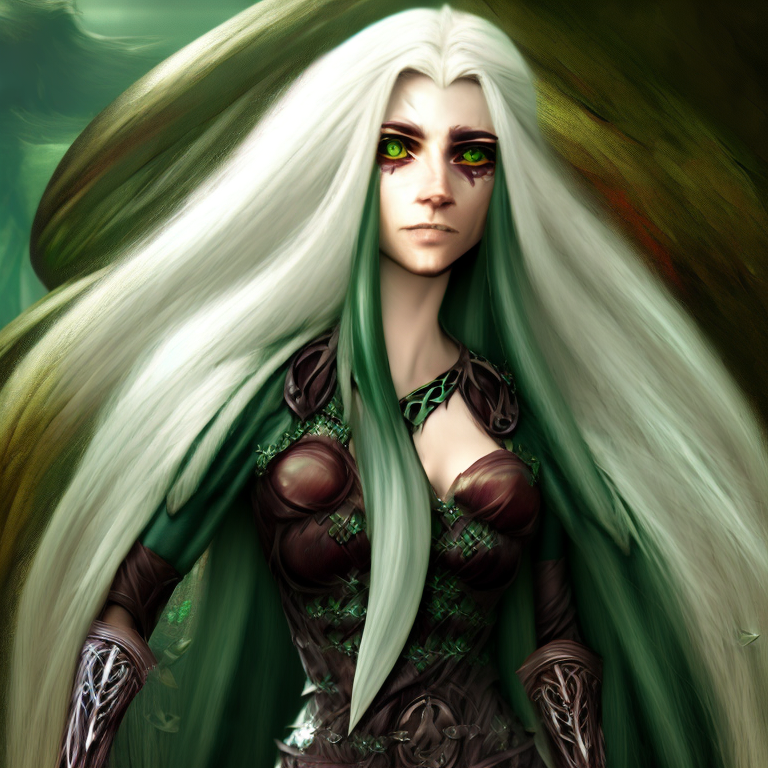
\includegraphics{full-body-portrait-of-a-beautiful-female-elf-with-long-silver-hairs-and-deep-green-eyes-fantasy-se-.png}
\caption{full-body-portrait-of-a-beautiful-female-elf-with-long-silver-hairs-and-deep-green-eyes-fantasy-se-.png}
\end{figure}

{[}Location{]} is the largest {[}location type{]} in the {[}larger
location{]} within the {[}geographic area{]} of {[}larger geographic
area{]}. {[}Location{]} neighbors {[}other location{]} to the
{[}direction{]} and {[}other location{]} to the {[}other direction{]}.
Known for being a place of {[}description{]}, {[}location{]} is home to
{[}people group{]} and the {[}organization{]}.

\begin{quote}
Citazione {[}location{]}
\end{quote}

\subsection{Biografia}\label{biografia}


The {[}people group{]} were the region's sole residents prior to the
{[}historical event{]}. {[}New people group{]} arrived in the region
around {[}year{]}.

\subsection{Carriera}\label{carriera}


The history and economic growth of {[}location{]} is tied to
{[}geographic feature{]} which is {[}location's{]} defining
characteristic.

\subsection{Personalità}\label{personalituxe0}



\section{Mortimer}\label{mortimer}


\begin{figure}
\centering
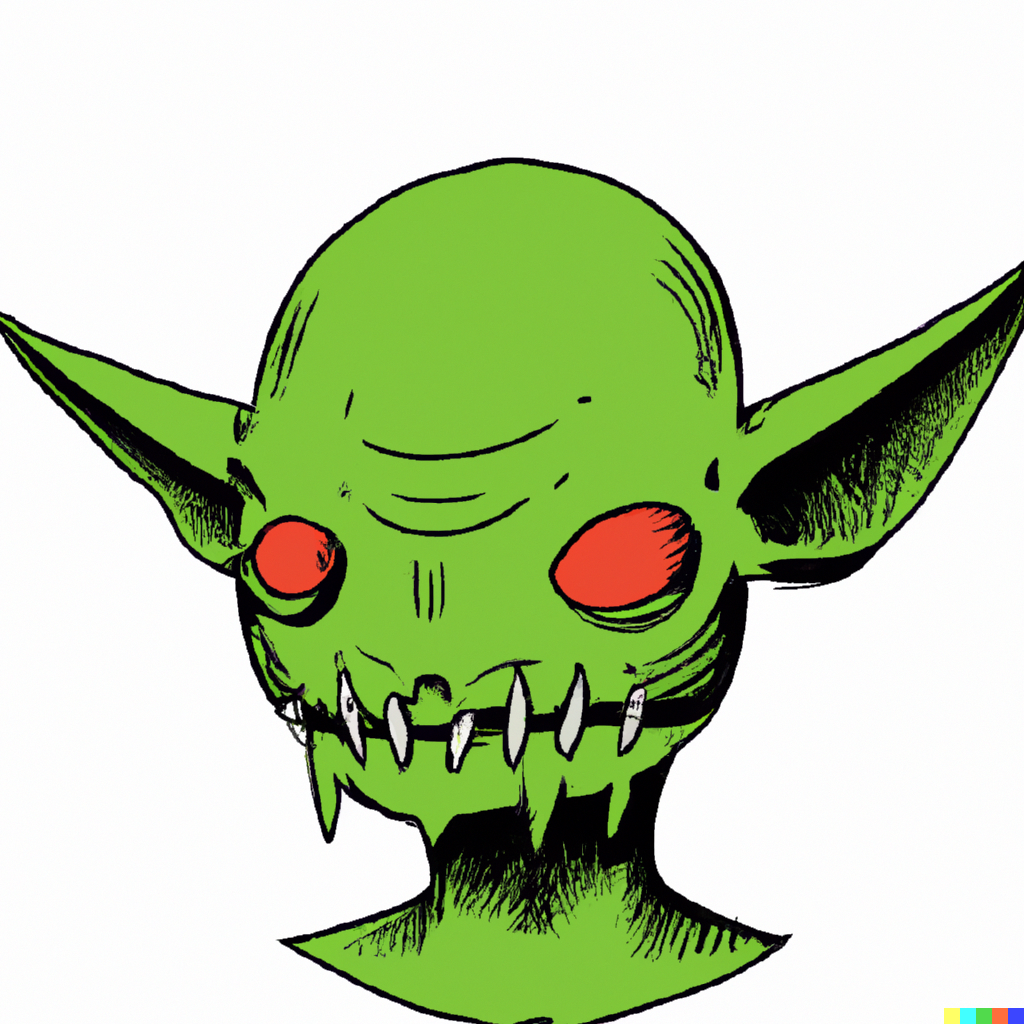
\includegraphics{Mortimer.png}
\caption{Mortimer.png}
\end{figure}

{[}Info generali{]}

Età: 12

Anno di nascita: 2011

Paese di nascita:

Razza: Goblin

Relazioni: Gilda dei Protettori

Alleati:

Nemesi:

Possedimenti importanti:


\subsection{Descrizione Generale}\label{descrizione-generale}


\begin{figure}
\centering
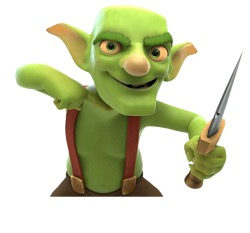
\includegraphics{Goblins_card_render.jpeg}
\caption{Goblins\_card\_render.jpeg}
\end{figure}

Un guerriero goblin con disturbo dell'attenzione.

\begin{quote}
``Voglio assaggiare quest'acqua di fogna''
\end{quote}

\subsection{Biografia}\label{biografia}


\begin{figure}
\centering
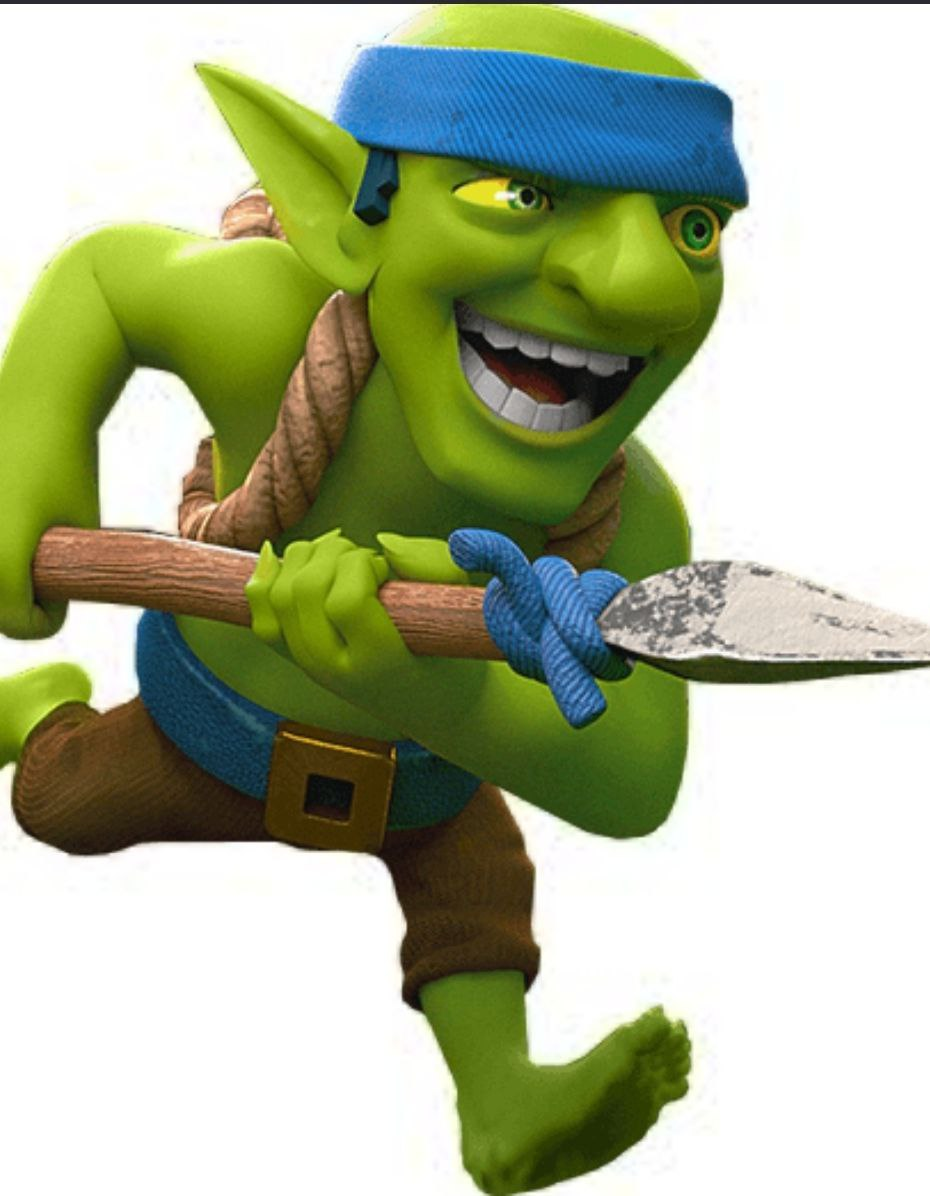
\includegraphics{2023-03-26_17.20.08.jpg}
\caption{2023-03-17.20.08.jpg}
\end{figure}

I genitori lo hanno mandato all'accademia militare con la speranza che
apprendesse disciplina e educazione, ma è scappato dopo un anno.

I genitori ancora lo cercano.

Per guadagnarsi da vivere ha scelto la strada più facile e sbagliata: il
crimine. Non ha legami con alcuna organizzazione in particolare,ma ha
dei contatti nella mala. Ogni tanto lo chiamano per dei lavori,
principalmente colpi a diligenze.

\subsection{Carriera}\label{carriera}


Nell'ultimo periodo si è affiliato alla Gilda dei Protettori della Sila
devoti a San Francesco e ai Lupi, un buon ``tetto sulla testa e una paga
decente'' a suo parere.

\subsection{Personalità}\label{personalituxe0}


Non ha ben in mente cosa sia bene e male, ma non perchè sia un goblin
(basta con gli stereotipi), viene da una famiglia per bene, gente che
gli ha dato un fior fiore di educazione\ldots{} Proprio è una testina di
cazzo.


\section{Pippo Francfrog}\label{pippo-francfrog}


\begin{figure}
\centering
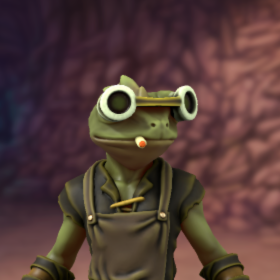
\includegraphics{Pippo_Francfrog-Token.png}
\end{figure}

\subsection{Descrizione Generale}\label{descrizione-generale}



Pippo Francfrog incarna l'incantevole fusione di una rana umanoide e la
magia dell'intrattenimento. La sua pelle iridescente rivela radici
anfibie, mentre lo sguardo intelligente brilla di carisma. Con abiti
vivaci e un sorriso contagioso, Pippo attrae l'attenzione ovunque vada.
La sua natura di artista si riflette in ogni gesto, mantenendo viva la
luce del palcoscenico anche mentre esplora nuovi orizzonti.

\begin{quote}
``Torte in faccia!''
\end{quote}

\subsection{Biografia}\label{biografia}


\subsubsection{Infanzia e le OriginiMistiche}\label{infanzia-e-le-origini-mistiche}
Pippo Francfrog vide la luce grazie a un incantesimo complesso e ardito
lanciato dal mago Lasalmadi Mikebongiorno. La sua creazione era un
tentativo di fondere la magia con il mondo dell'intrattenimento,
producendo così una creatura unica nel suo genere. Sin dalla sua
nascita, Pippo ha portato con sé un legame con la magia che avrebbe
influenzato il corso della sua vita.

\subsubsection{Esordi in ``Il Bagaglione''}
I primi passi di Pippo nel mondo dell'intrattenimento li compì entrando
a far parte dello spettacolo itinerante de ``Il Bagaglione''. Qui, Pippo
fu introdotto all'arte dell'intrattenimento e imparò i segreti
dell'interazione con il pubblico. Le sue performance coinvolgenti e
innovative catturarono l'attenzione di tutti coloro che ebbero la
fortuna di assistere ai suoi numeri.

\subsubsection{Richiamo della Magia e il Percorso come Artificiere}
Mentre il suo talento nel campo dell'intrattenimento si faceva sempre
più evidente, la sua connessione con la magia iniziò a emergere in modo
più preponderante. Sentendo il richiamo della magia dentro di sé, Pippo
intraprese un nuovo cammino come artificiere. La sua abilità nel creare
oggetti incantati e invenzioni uniche gli permise di esprimere la sua
creatività in modi mai sperimentati prima.

\subsubsection{Unione Fraterna con Pippo Baudog}
Le avventure di Pippo non furono mai solitarie. Insieme a suo fratello
Pippo Baudog, un cane antropomorfo con il medesimo retaggio magico,
intraprese molte imprese. La loro partnership rappresentava l'armoniosa
fusione tra intrattenimento e abilità magica, dimostrando il valore
dell'affetto fraterno nel raggiungimento dei traguardi.

\subsubsection{Eredità e Impatto}
La vita di Pippo Francfrog è rimasta una testimonianza dell'incrocio tra
il mondo della magia e dell'intrattenimento. La sua biografia incarna la
perseveranza nella ricerca della propria passione, nonostante le diverse
sfaccettature della sua identità. La sua eredità continua a ispirare
coloro che cercano di fondere passioni divergenti, aprendo la strada a
un mondo di meraviglia, sorpresa e collaborazione.

\subsection{Carriera}\label{carriera}


La carriera di Pippo Francfrog è stata un connubio straordinario tra
magia e intrattenimento. Dopo esordi di successo con lo spettacolo
itinerante de ``Il Bagaglione'', Pippo ha seguito il richiamo della
magia e si è dedicato all'artigianato magico come artificiere.
Nonostante questo cambiamento di percorso, non ha mai dimenticato le sue
radici da intrattenitore, portando sempre con sé il desiderio di
incantare e stupire il pubblico. Collaborando spesso con suo fratello,
Pippo Baudog, ha dimostrato come la fusione di talento e creatività
possa creare un'esperienza unica e indimenticabile per chiunque lo
incontri. La sua carriera è un esempio di come diverse passioni possano
coesistere e arricchirsi a vicenda, creando un mondo di meraviglia e
sorpresa.

\subsection{Personalità}\label{personalituxe0}


La personalità di Pippo Francfrog è un affascinante mix di carisma,
curiosità e creatività. È un individuo straordinariamente affabile, con
un sorriso contagioso e uno sguardo che riflette un'intelligenza
brillante. La sua natura di intrattenitore è evidente in ogni aspetto
della sua vita, portando con sé l'abilità di incantare e stupire
chiunque incontri. La sua curiosità insaziabile lo spinge a esplorare
nuovi orizzonti, sia nell'arte dello spettacolo che nell'artigianato
magico. Tuttavia, il suo cuore rimane fedele al desiderio di portare
gioia e meraviglia al pubblico, e questa passione è il motore che guida
ogni sua azione. La sua personalità è un richiamo costante alla magia
della creatività e all'importanza di diffondere la gioia attraverso
l'arte e lo spettacolo.


\section{Sabaku no Darude}\label{sabaku-no-darude}


\begin{figure}
\centering
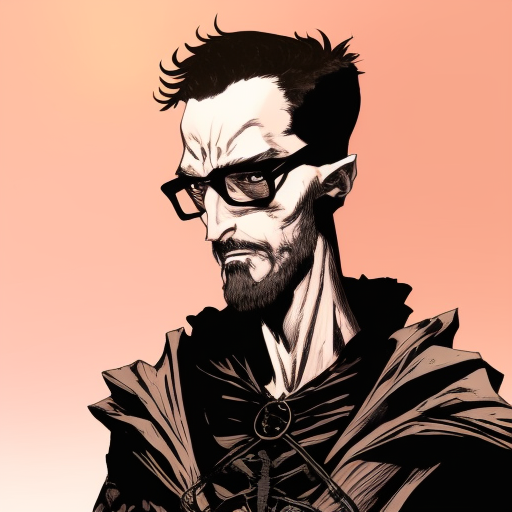
\includegraphics{blkmndy_fantasy_character_with_a_hooded_cape_with_a_beard_with_glasses.png}
\end{figure}

\subsection{Descrizione Generale}\label{descrizione-generale}



Sabaku no Darude è un mezzelfo nato in una landa desertica del
continente. Ha una combinazione di tratti sia umani che elfici, con una
pelle leggermente scura e capelli castani mossi. I suoi occhi, di un
colore ambrato brillante, riflettono la sua passione interiore.

\begin{quote}
``Per chi conosce la Lore. Per chi la sta scoprendo. Per chi la
scoprirà'' - Sabaku no Darude
\end{quote}

\subsection{Biografia}\label{biografia}


Sabaku no Darude è cresciuto in una landa desertica dopo la morte dei
suoi genitori mercenari quando aveva solo 5 anni. Ha vissuto con il suo
saggio nonno materno, un elfo che gli ha trasmesso l'amore per la musica
e l'arte. Grazie alle storie epiche e alle ballate antiche che ha
ascoltato, Darude ha sviluppato un profondo desiderio di condividerle
con tutte le razze del mondo.

\subsection{Carriera}\label{carriera}


Per realizzare il suo desiderio di diffondere conoscenza e creare un
legame tra le persone, Darude ha intrapreso un viaggio come bardo
itinerante. Durante i suoi viaggi, esplora nuovi luoghi, impara le
storie locali e interagisce con le diverse culture e razze. Durante
queste esperienze, scrive di sé stesso e degli avvenimenti che gli
accadono intorno, creando un diario di viaggio personale.

Darude si esibisce in vari luoghi, dalle taverne dei villaggi alle corti
dei re, utilizzando la sua abilità musicale e le sue doti di narratore
per coinvolgere il pubblico. La sua musica tocca le corde dell'anima e
le sue storie ispirano gli ascoltatori a guardare al di là delle
differenze e a trovare un terreno comune.

\subsection{Personalità}\label{personalituxe0}


Darude è una persona gentile e appassionata, con una grande curiosità e
apertura mentale. È rispettoso delle tradizioni locali e cerca sempre di
creare comprensione reciproca tra le diverse razze. La sua passione per
la musica e le storie è contagiosa e porta gioia ovunque vada. Ha
un'anima creativa e un cuore generoso, e cerca di utilizzare le sue
abilità per rendere il mondo un posto migliore.


\section{Stalag Might}\label{stalag-might}


\begin{figure}
\centering
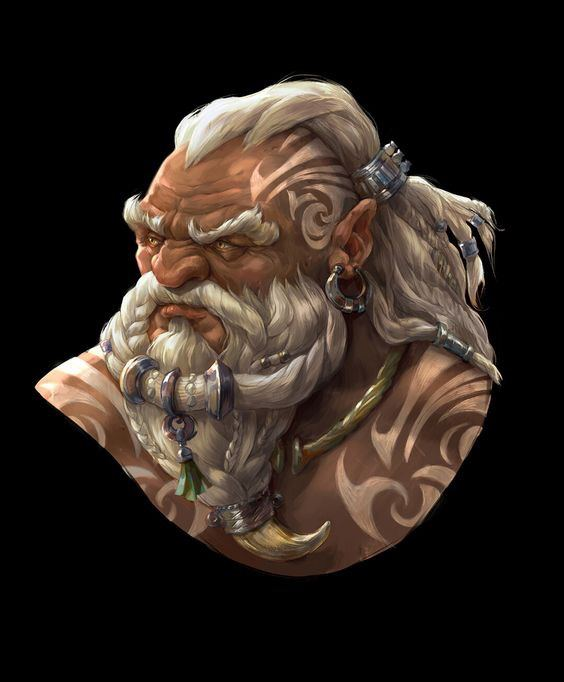
\includegraphics{2023-09-17_22.34.48.jpg}
\end{figure}

\subsection{Descrizione Generale}\label{descrizione-generale}


Stalag Might è un nano druido le cui origini sono radicate nelle
profondità di una montagna antica conosciuta come ``Lunacrest''. La sua
storia è intrecciata con il mistero di questa montagna, dove le energie
dell'antica luna scorrono nelle vene stesse della terra. Conosciuto tra
i druidi come il ``Bambino delle Rocce'', Stalag ha sempre mostrato una
connessione innata con le pietre e una passione per la geologia.

\begin{quote}
``Bella questa roccia''
\end{quote}

\subsection{Biografia}\label{biografia}


\subsubsection{Infanzia}\label{infanzia}


Stalag Might nacque nelle viscere di Lunacrest, portando con sé una
strana formazione rocciosa sulla mano sinistra, simile alle maestose
montagne circostanti. Questo segno innato attirò l'attenzione dei suoi
genitori, che lo condussero alla congrega dei druidi del Circolo della
Luna quando era ancora un neonato. Il giovane nano cresceva, diventando
noto tra i druidi come il ``Bambino delle Rocce''. La sua forza fisica e
la sua passione per la geologia lo resero un apprendista straordinario.

\subsubsection{Adolescenza}\label{adolescenza}


Durante gli anni della sua formazione, Stalag sviluppò un profondo
interesse per la metamorfosi, una delle abilità centrali dei druidi del
Circolo della Luna. A differenza dei suoi compagni, prediligeva
trasformarsi in piccoli animali, come topi, talpe e lucertole, per
esplorare fessure e cavità inaccessibili. Questa abilità gli consentiva
di scoprire gemme nascoste e segreti geologici, e raccontava avventure
vissute attraverso gli occhi di un piccolo animale.

\subsubsection{Età Adulta}\label{etuxe0-adulta}


Durnan Crystalbeard, il suo anziano maestro druido, riconoscendo il
talento e la dedizione di Stalag, gli regalò un geode speciale quando il
giovane nano compì sedici anni. Questo geode, inciso con simboli
druidici, divenne sia un focus per la sua magia che un santuario per
campioni di rocce e minerali rari. Dopo aver completato la sua
formazione con la congrega, Stalag sentì il richiamo dell'esplorazione e
del desiderio di scoprire montagne e formazioni rocciose leggendarie,
alla ricerca in particolare della pietra leggendaria nota come ``Il
Cuore della Luna''.

\subsection{Personalità}\label{personalituxe0}


Stalag Might è noto per la sua mente curiosa e la passione incrollabile
per la geologia. È un individuo tranquillo ma osservatore, sempre
desideroso di ascoltare le storie delle pietre e dei minerali che
incontra lungo il suo cammino. La sua connessione con la natura e il
mondo sotterraneo lo rende rispettoso nei confronti dell'ambiente
circostante.

Inoltre, la sua abilità unica di trasformarsi in creature più piccole
gli conferisce una prospettiva unica sulla vita e sull'esplorazione.
Stalag è affezionato ai suoi compagni druidi e considera ogni avventura
come un'opportunità per arricchire la sua comprensione delle meraviglie
naturali del mondo.

Stalag Might è guidato da una doppia missione: la sete di conoscenza
geologica e la ricerca dell'enigmatica ``Pietra della Luna''. Questo
equilibrio tra scienza e magia guida le sue azioni mentre viaggia
attraverso il mondo, pronta a esplorare e a svelare i segreti che
attendono sotto le rocce e nelle profondità della terra.



\chapter{Personaggi non giocanti}
\newpage
%
\section{Enzhosor Ent Ino}\label{enzhosor-ent-ino}

Tags: NPC Alias: Il Satiro Creatore: Davide Ispirazione: Enzo Sorrentino
Luogo: Valtorria Razza: Elfo Classe: Bardo

\section{Enzhosor Ent Ino}\label{enzhosor-ent-ino-1}

\begin{center}\rule{0.5\linewidth}{0.5pt}\end{center}

\begin{figure}
\centering
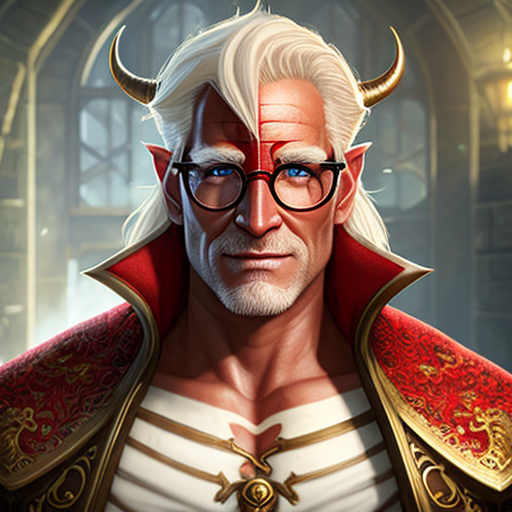
\includegraphics{a-male-tiefling-red-skin-and-blonde-hair-old-age-spectacles-.png}
\caption{a-male-tiefling-red-skin-and-blonde-hair-old-age-spectacles-.png}
\end{figure}

Informazioni Generali

Età: 62

Anno di nascita: 1961

Paese di nascita:

Razza: Mezzo tiefling

Professione: Sindaco

Alleati:

Nemesi:

Possedimenti importanti:

Conosciuto come: Il regista

\begin{center}\rule{0.5\linewidth}{0.5pt}\end{center}

\subsection{1. Descrizione Generale}\label{descrizione-generale}

\begin{center}\rule{0.5\linewidth}{0.5pt}\end{center}

\begin{figure}
\centering
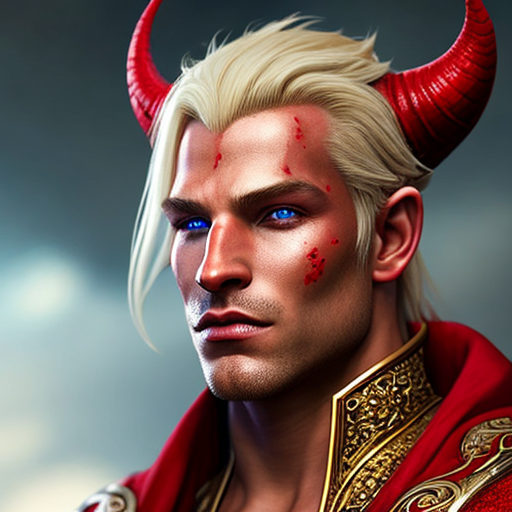
\includegraphics{a-male-tiefling-red-skin-and-blonde-hair-.png}
\caption{a-male-tiefling-red-skin-and-blonde-hair-.png}
\end{figure}

Enzhosor Ent Ino è un uomo di 62 anni, con capelli bianchi e crespi che
circondano la sua testa come una criniera. È un individuo dall'aspetto
fiero, con una statura media e una postura eretta. Indossa sempre abiti
eleganti e colorati, spesso arricchiti da gioielli e dettagli sontuosi.
I suoi occhi chiari, vivaci e intelligenti, riflettono la determinazione
che lo caratterizza.

\begin{quote}
``Satira!''
\end{quote}

\subsection{2. Biografia}\label{biografia}

\begin{center}\rule{0.5\linewidth}{0.5pt}\end{center}

Enzhosor è nato e cresciuto nella città di Valtorria, che un tempo era
un importante centro commerciale della regione. Sin da giovane, ha
dimostrato una grande passione per le arti drammaturgiche. Ha trascorso
la sua giovinezza viaggiando, portando il suo teatro tra le città e
villaggi di Valtara. Nonostante la sua forte autostima, le sue doti non
sono mai state apprezzate, ed in seguito ad uno spiacevole incidente, è
stato costretto a tornare a casa.

\subsubsection{2.1 Il fatale incidente}\label{il-fatale-incidente}

Durante uno dei suoi epici viaggi insieme alla sua compagnia teatrale,
Enzhosor si trovò improvvisamente costretto ad attraversare un antico
sentiero di montagna. La via, avvolta da un velo di mistero e gelo, si
stagliava sinistra e stretta, mentre il carro galleggiava sopra la
superficie ghiacciata. Il destriero di Enzhosor, aggraziato quanto un
unicorno, tentò invano di mantenere la presa, ma l'impeto
incontrollabile lo spinse verso l'abisso senza pietà.

Con un balzo acrobatico, Enzhosor si lanciò nell'aria, sfidando la
gravità e gli spiriti maligni che popolavano quei luoghi sconosciuti.
L'aura di un'antica profezia lo guidò verso un approdo sicuro,
salvandolo da un destino avverso. Tuttavia, il destino non ebbe pietà
per il resto della sua fida compagnia, imprigionata all'interno del
carro in fuga.

L'evento tragico, ancora oggi pesante nel cuore di Enzhosor, si rivelò
una scossa che sconvolse il suo spirito avventuroso. Decideva così di
porre fine alla sua vita come artista itinerante, abbandonando le strade
erranti per fare ritorno a Valtorria, un regno lontano, in cerca di
serenità e riscatto.

\subsection{3. Carriera}\label{carriera}

\begin{center}\rule{0.5\linewidth}{0.5pt}\end{center}

Dopo aver acquisito un'ampia conoscenza dell'animo umano, Enzhosor ha
deciso di stabilirsi a Valtorria e intraprendere una carriera politica.
Grazie alla sua capacità di negoziare e alle sue abilità di leadership,
è riuscito a diventare il sindaco della città. Da allora, ha concentrato
i suoi sforzi nell'ampliare il potere di Valtorria e aumentare la sua
influenza economica.

Enzhosor ha avviato molte iniziative per promuovere lo sviluppo
economico di Valtorria, come la creazione di nuovi mercati, l'attrazione
di investimenti e la promozione di alleanze commerciali con altre città.
Tuttavia, il suo desiderio di conquistare Azura per il controllo
completo dei commerci marittimi ha reso la sua politica più aggressiva e
ambiziosa.

\begin{figure}
\centering
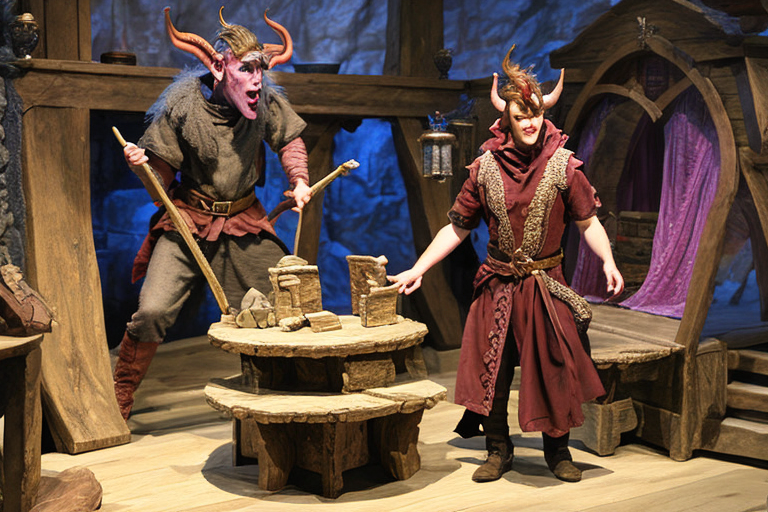
\includegraphics{a-fantasy-theatre-with-a-male-tiefling-playing--2.png}
\caption{a-fantasy-theatre-with-a-male-tiefling-playing--2.png}
\end{figure}

\subsection{4. Personalità}\label{personalituxe0}

\begin{center}\rule{0.5\linewidth}{0.5pt}\end{center}

Enzhosor è un uomo sicuro di sé, determinato e ambizioso. È convinto di
essere l'uomo più divertente del mondo, anche se spesso il suo senso
dell'umorismo è considerato piuttosto discutibile dagli altri. Adora
raccontare barzellette, inventarne di nuove e sorridere a se stesso
mentre le racconta, ma spesso le sue battute sono considerate forzate o
poco riuscite dagli altri.

Nonostante la sua personalità dominante e la sete di potere, Enzhosor è
anche un individuo intelligente e strategico. È abile nel riconoscere le
opportunità economiche e sa come sfruttarle a suo vantaggio. Tuttavia,
la sua brama di potere può portarlo a prendere decisioni poco etiche o a
ignorare il benessere degli altri.

In conclusione, Enzhosor Ent Ino è un sindaco ambizioso e carismatico,
determinato a espandere l'influenza di Valtorria. La sua personalità
carismatica e il suo senso dell'umorismo discutibile lo rendono un
personaggio interessante e controverso, pronto a sfidare gli altri per
raggiungere i suoi obiettivi.

\begin{quote}
``Enzo chiede a Kos: Hey Enzo, sei stato a Kos? Ma Kos? Kosa dici?
\ldots{} Satira''
\end{quote}

\subsection{A. Coinvolgimenti in eventi
recenti}\label{a.-coinvolgimenti-in-eventi-recenti}

\begin{center}\rule{0.5\linewidth}{0.5pt}\end{center}

\href{Untitled\%20Database\%20b540a0577b624713b0d8ac194cd482f5.csv}{Untitled
Database}

\subsection{B. Aggiornamenti}\label{b.-aggiornamenti}

\begin{center}\rule{0.5\linewidth}{0.5pt}\end{center}

\href{Untitled\%205bbba70bc8d14d398e68283ff572fd85.csv}{}

\section{Fran}\label{fran}

Tags: NPC, Quartiermastro Creatore: Lorenzo

\section{Fran}\label{fran-1}

\begin{center}\rule{0.5\linewidth}{0.5pt}\end{center}

\begin{figure}
\centering
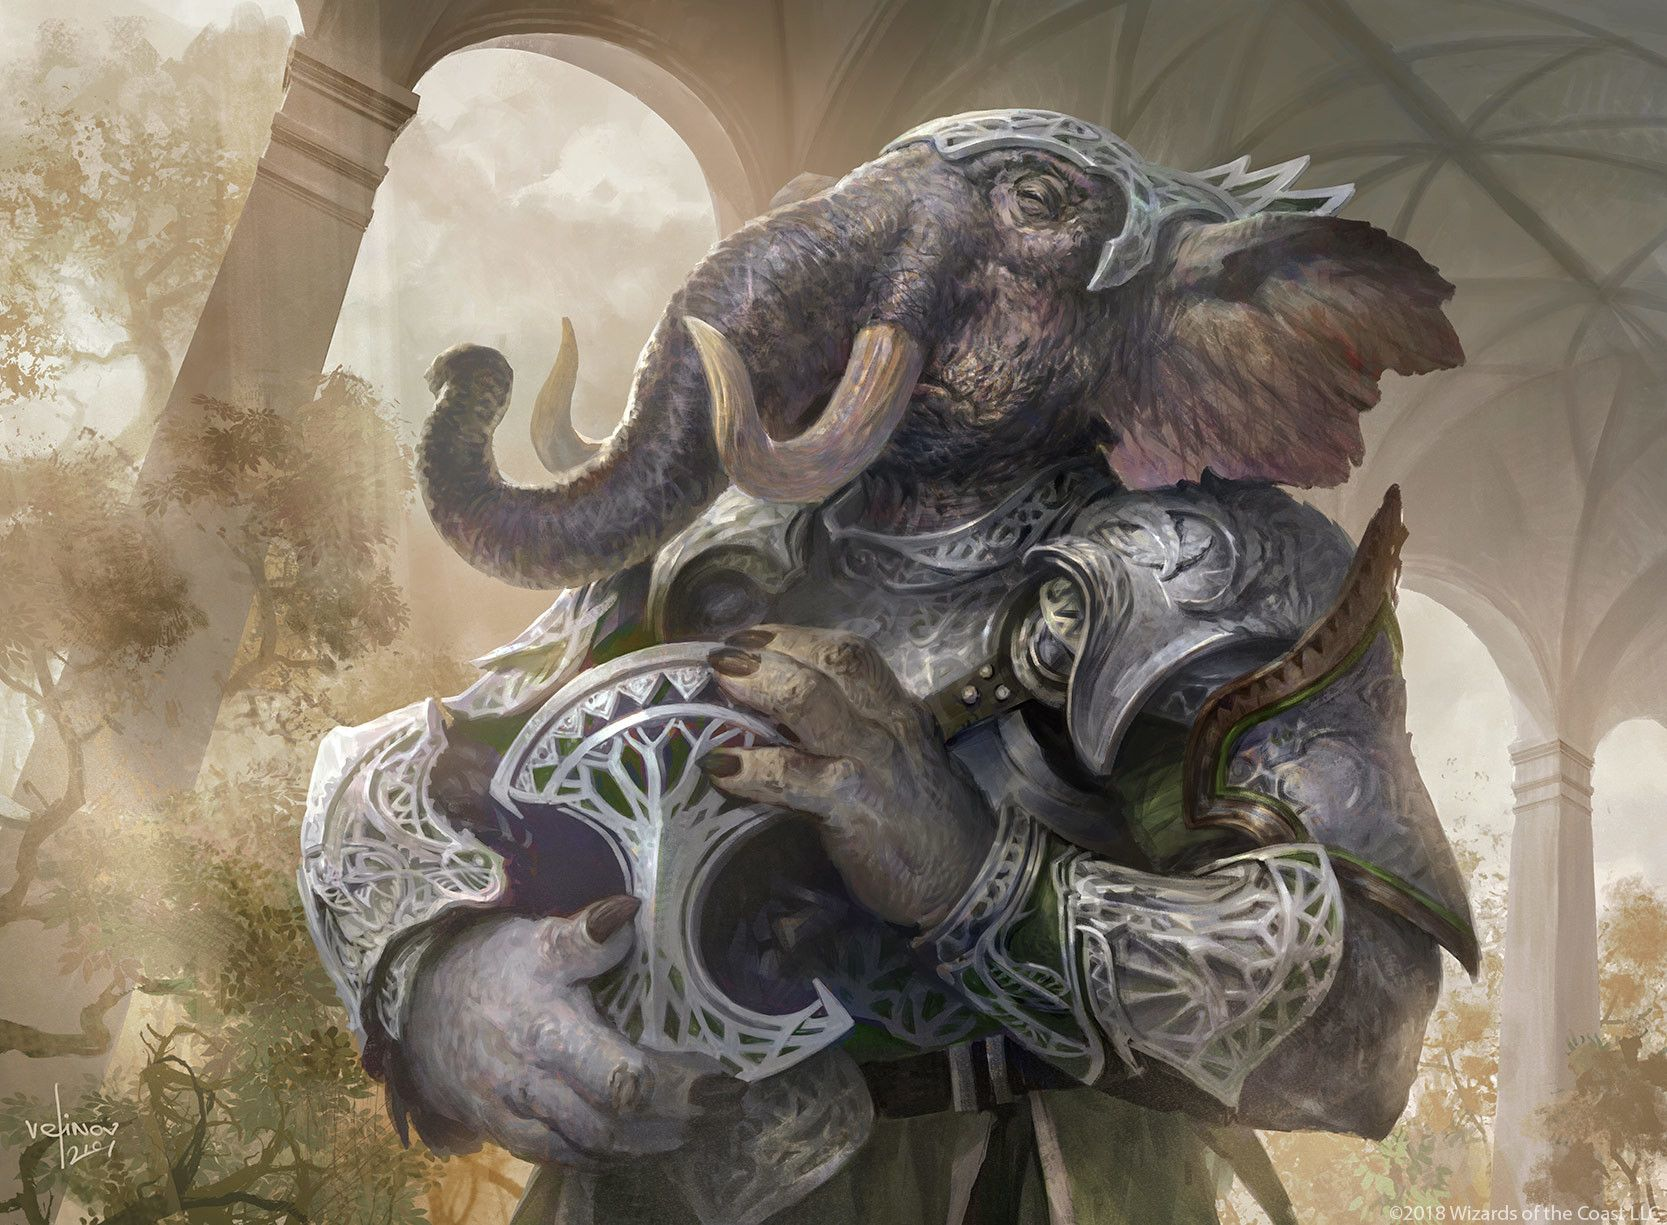
\includegraphics{crisro_redentore_vaffanculio_stronawoqijoaoijpaef.jpg}
\caption{crisro redentore vaffanculio stronawoqijoàaoijpaef.jpg}
\end{figure}

Informazioni Generali

Anno di nascita: 1776

Paese di nascita: Foresta degli Elefarici

Razza: Lossodonte

Relazioni:

Alleati:

Nemesi:

Possedimenti importanti:

\begin{center}\rule{0.5\linewidth}{0.5pt}\end{center}

\subsection{1. Descrizione Generale}\label{descrizione-generale}

\begin{center}\rule{0.5\linewidth}{0.5pt}\end{center}

Fran è il quartiermastro della Gilda dei Protettori di Eldrid.

\begin{figure}
\centering
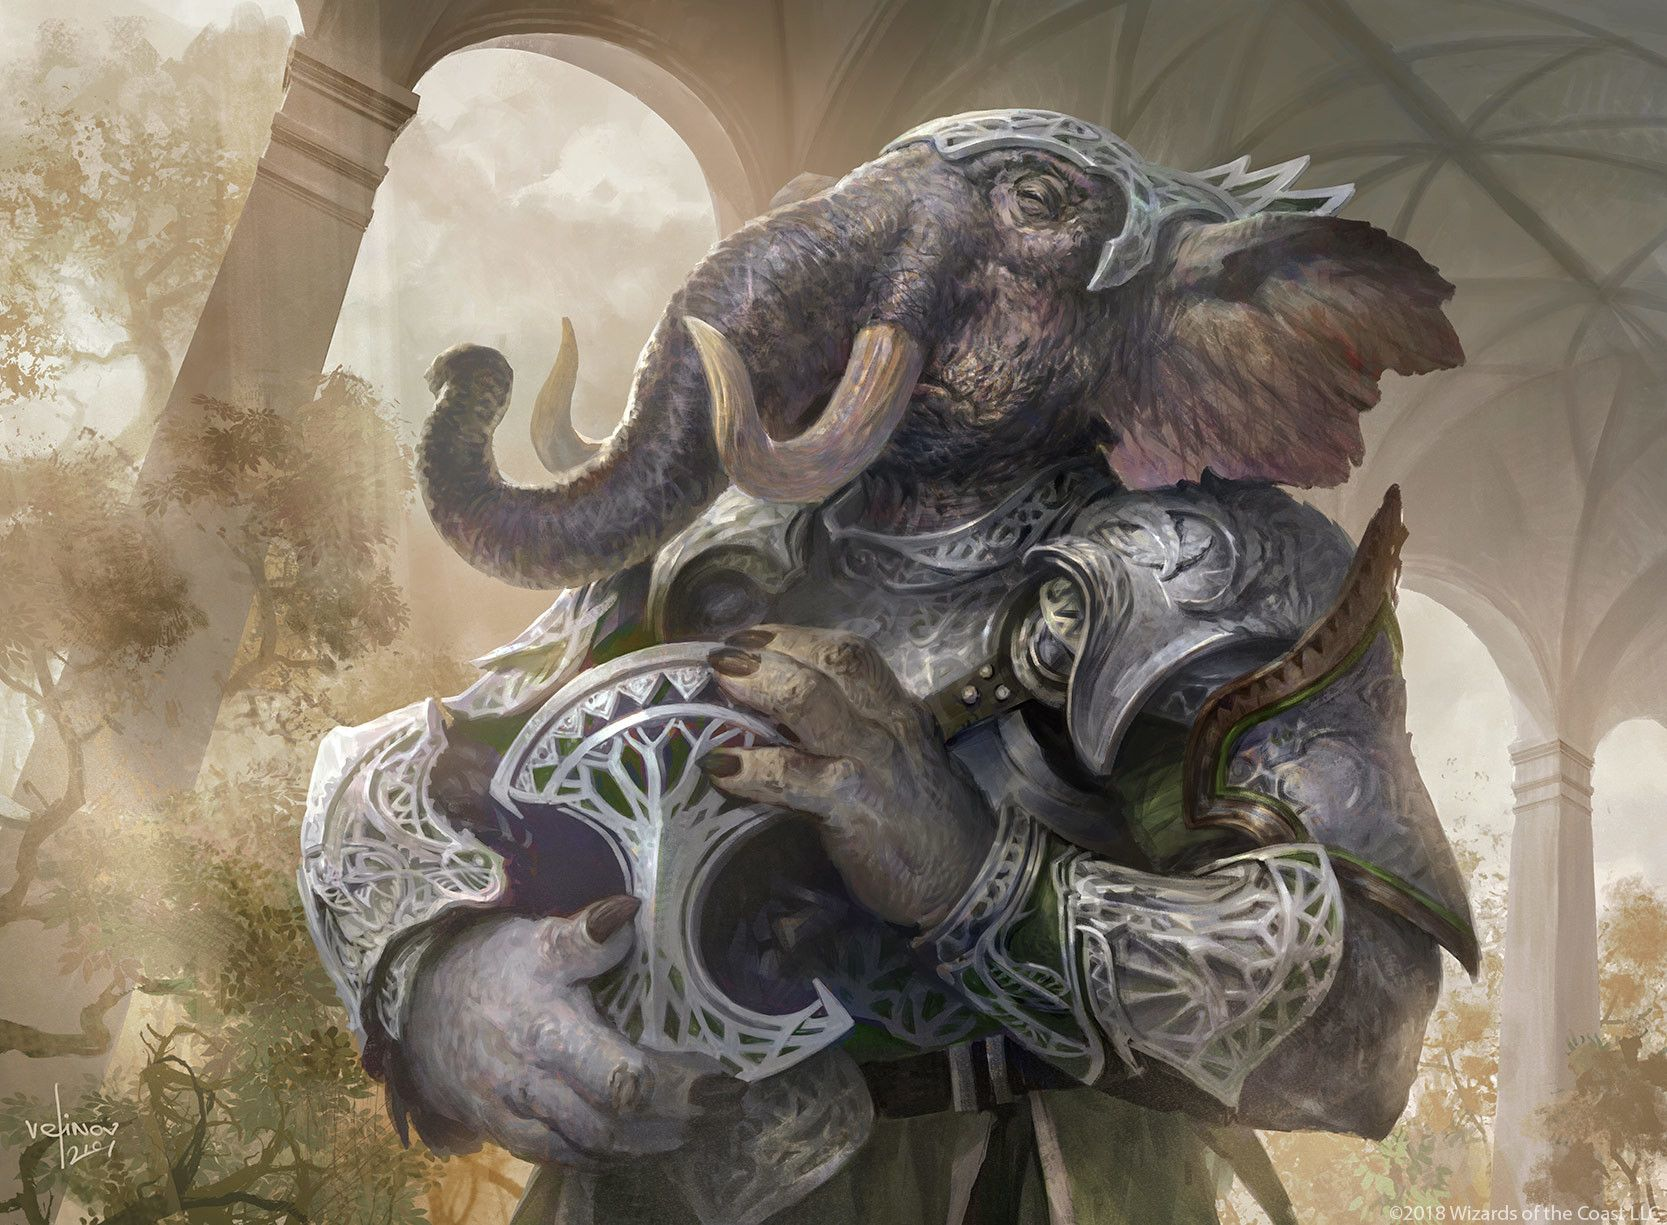
\includegraphics{crisro_redentore_vaffanculio_stronawoqijoaoijpaef 1.jpg}
\caption{crisro redentore vaffanculio stronawoqijoàaoijpaef.jpg}
\end{figure}

Fran è un lossodonte dall'aspetto imponente, con un corpo massiccio e
una pelle grigia rugosa che gli conferisce un'aria saggia. Nonostante la
sua mole, è sorprendentemente agile e porta sempre con sé un mantello
colorato con frange e ricami eccentrici. Indossa un'armatura
personalizzata, progettata appositamente per adattarsi alla sua figura
robusta. Porta sempre con se un piccolo baule, contenente tutto il
necessario per le sue responsabilità di quartiermastro della gilda dei
Protettori.

\subsection{2. Biografia}\label{biografia}

\begin{center}\rule{0.5\linewidth}{0.5pt}\end{center}

Fran è nato nella lussureggiante foresta degli Elefarici, una terra
d'oltreoceano abitata da lossodonti. Crescendo, ha sviluppato una
passione per l'esplorazione, che lo ha portato fino a Eldrid. Dopo aver
appreso delle gesta dei Protettori, ha deciso di unirsi a loro e mettere
le sue abilità al servizio della gilda.

\subsection{3. Carriera}\label{carriera}

\begin{center}\rule{0.5\linewidth}{0.5pt}\end{center}

Dopo aver dimostrato la sua abilità nelle missioni di combattimento,
Fran è stato nominato quartiermastro della gilda dei Protettori di
Eldrid. Con la sua natura socievole, è riuscito a stringere amicizia con
mercanti e commercianti, ottenendo sconti incredibili per le ultime
novità sul mercato.

\subsection{4. Personalità}\label{personalituxe0}

Fran è un lossodonte dal cuore tenero e un gran senso dell'umorismo.
Anche se il suo aspetto intimidatorio potrebbe far pensare il contrario,
è amato e rispettato dai membri della gilda per il suo spirito allegro e
la sua capacità di alleviare la tensione durante le missioni pericolose.
Spesso scherza sul suo aspetto mastodontico, definendosi ``l'elefante
nella stanza''. Nonostante la sua comicità, Fran è un individuo
estremamente competente e leale, sempre pronto a difendere i suoi
compagni con la sua forza e astuzia.

La combinazione unica di abilità di combattimento, competenza
organizzativa e personalità gioiosa rende Fran un membro essenziale
della gilda dei Protettori di Eldrid. La sua presenza nella squadra
porta un senso di calma e fiducia, e i suoi amici sanno di poter contare
su di lui sia come compagno di avventure che come responsabile delle
risorse.

\begin{center}\rule{0.5\linewidth}{0.5pt}\end{center}

\subsection{A. Coinvolgimenti in eventi
recenti}\label{a.-coinvolgimenti-in-eventi-recenti}

\begin{center}\rule{0.5\linewidth}{0.5pt}\end{center}

\href{Untitled\%20Database\%20c977bec678f84b799a4925770fa66698.csv}{Untitled
Database}

\subsection{B. Aggiornamenti}\label{b.-aggiornamenti}

\begin{center}\rule{0.5\linewidth}{0.5pt}\end{center}

\href{Untitled\%208bd95847a17f4fb69a1aba05ab5418f7.csv}{}

\section{Gi Mi 1}\label{gi-mi-1}

Tags: NPC Creatore: Davide Ispirazione: Gimmi Ghione Razza: Elfo Classe:
Ranger-Mago

\section{Gi Mi 1}\label{gi-mi-1-1}

\begin{center}\rule{0.5\linewidth}{0.5pt}\end{center}

\begin{figure}
\centering
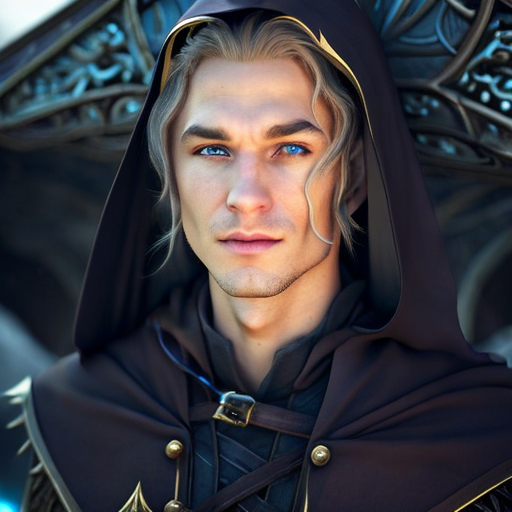
\includegraphics{hooded-fantasy-elf-.png}
\caption{hooded-fantasy-elf-.png}
\end{figure}

Informazioni Generali

Età:

Anno di nascita:

Paese di nascita:

Razza: Elfo

Relazioni: La Striscia della Notizia

Alleati: Gilda dei protettori

Nemesi: Il male

Possedimenti importanti:

\begin{center}\rule{0.5\linewidth}{0.5pt}\end{center}

\subsection{1. Descrizione Generale}\label{descrizione-generale}

\begin{center}\rule{0.5\linewidth}{0.5pt}\end{center}

\begin{figure}
\centering
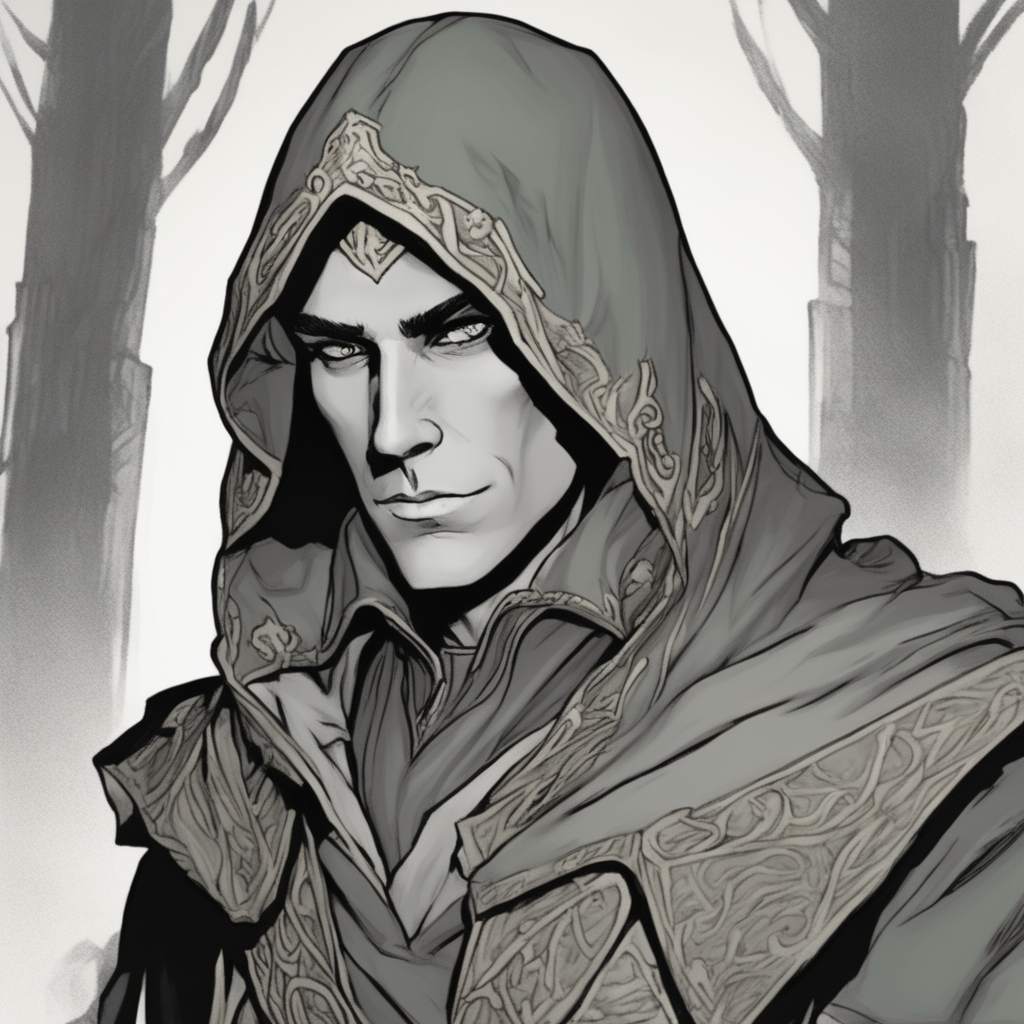
\includegraphics{create-a-portrait-style-image-of-elrandir-an-elven-operative-from-the-news-strip-in-a-covert-sit.png}
\caption{create-a-portrait-style-image-of-elrandir-an-elven-operative-from-the-news-strip-in-a-covert-sit.png}
\end{figure}

Gi Mi 1 è un elfo alto e slanciato, con un'aria discreta che gli
consente di passare inosservato tra la folla. Indossa abiti sobri e una
giacca che nasconde spesso strumenti e documenti utili per il suo lavoro
di spionaggio. I suoi occhi azzurri, pur riflettendo la sua
intelligenza, sono sempre attenti e vigili. La sua espressione è seria e
riservata, rivelandosi solo a chi è degno della sua fiducia.

\begin{quote}
Citazione {[}location{]}
\end{quote}

\subsection{2. Carriera}\label{carriera}

\begin{center}\rule{0.5\linewidth}{0.5pt}\end{center}

Gi Mi 1 è uno degli operatori principali di
\href{https://www.notion.so/La-Striscia-Della-Notizia-58157109cdb44626b1d92668711114d1?pvs=21}{La
Striscia Della Notizia} . Il suo ruolo consiste nel reperire
informazioni vitali che potrebbero minacciare l'equilibrio del mondo e
garantire che queste informazioni siano consegnate a chi può prevenire
le catastrofi imminenti. Lavora nell'ombra, spesso sotto falsa identità,
mentre compie missioni rischiose per proteggere la pace globale.

\subsection{3. Personalità}\label{personalituxe0}

\begin{center}\rule{0.5\linewidth}{0.5pt}\end{center}

Gi Mi 1 è noto per la sua dedizione assoluta al suo ruolo all'interno di
``La Striscia della Notizia''. È un individuo riservato, abituato a
lavorare nell'ombra e a mantenere un profilo basso. La sua intelligenza
è affilata come una lama e possiede una capacità innata di analizzare
situazioni e individuare informazioni vitali.

\subsection{A. Coinvolgimenti in eventi
recenti}\label{a.-coinvolgimenti-in-eventi-recenti}

\begin{center}\rule{0.5\linewidth}{0.5pt}\end{center}

\href{Untitled\%20Database\%2004658c200c5a4cedbb672aee61ba2af3.csv}{Untitled
Database}

\subsection{B. Aggiornamenti}\label{b.-aggiornamenti}

\begin{center}\rule{0.5\linewidth}{0.5pt}\end{center}

\href{Untitled\%20e444802359d547a8adcf33286185100d.csv}{}

\subsection{C. Galleria Immagini}\label{c.-galleria-immagini}

\begin{figure}
\centering
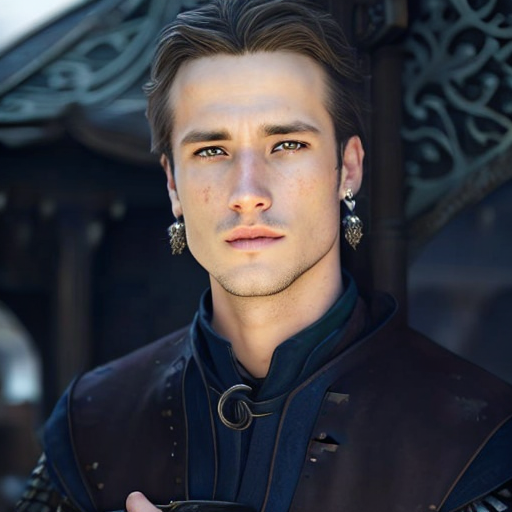
\includegraphics{a-fantasy-male-character-set-in-medieval-market-.png}
\caption{Gi Mi vanta una grande capacità nel cambiare taglio di capelli
per non farsi riconoscere}
\end{figure}

Gi Mi vanta una grande capacità nel cambiare taglio di capelli per non
farsi riconoscere

\section{Girolamo Giacomino
Gorgonzola}\label{girolamo-giacomino-gorgonzola}

Tags: NPC Alias: GGG Creatore: Davide Ispirazione: Geronimo Stilton; JJ
Jameson Luogo: Kos

\section{Girolamo Giacomino
Gorgonzola}\label{girolamo-giacomino-gorgonzola-1}

\begin{center}\rule{0.5\linewidth}{0.5pt}\end{center}

\begin{figure}
\centering
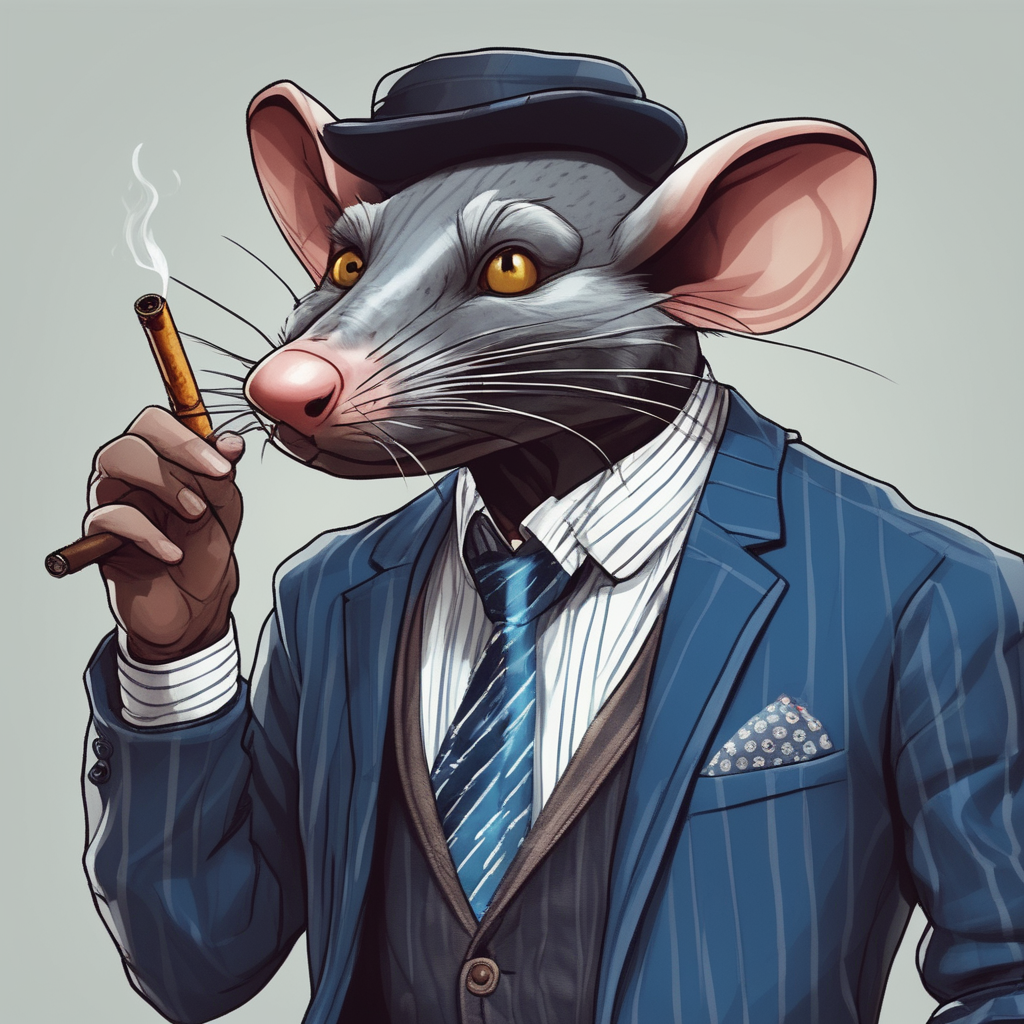
\includegraphics{create-an-image-of-a-human-folk-a-fantasy-race-with-humankind-features-resembling-a-rat-he-has-a-st.png}
\caption{create-an-image-of-a-human-folk-a-fantasy-race-with-humankind-features-resembling-a-rat-he-has-a-st.png}
\end{figure}

Informazioni Generali

Età: 44

Data di nascita: 26/12/1978

Luogo di nascita: Kos

Razza: Ratfolk

Professione: Giornalista

Alias: Un topo, anzi un tipo

\begin{center}\rule{0.5\linewidth}{0.5pt}\end{center}

\subsection{1. Descrizione Generale}\label{descrizione-generale}

\begin{center}\rule{0.5\linewidth}{0.5pt}\end{center}

\begin{figure}
\centering
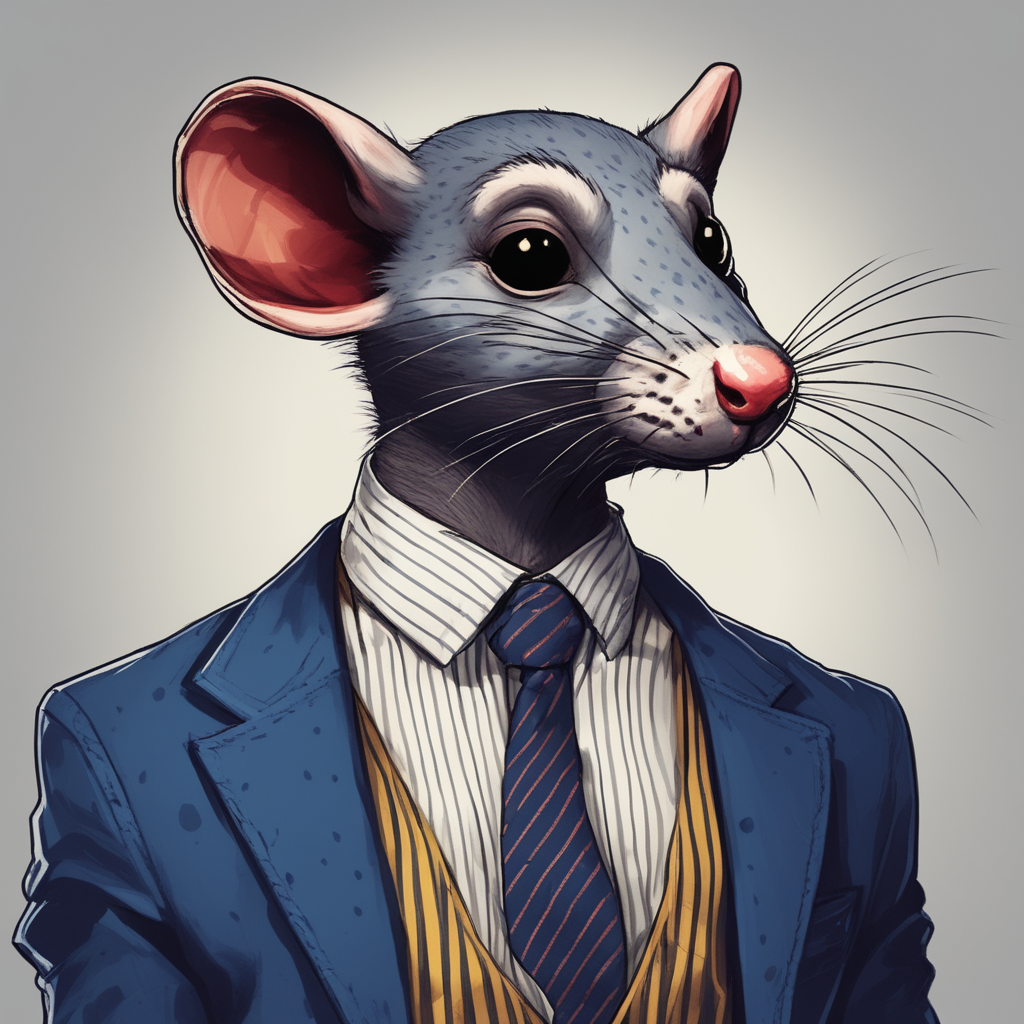
\includegraphics{create-an-image-of-a-human-folk-a-fantasy-race-with-humankind-features-resembling-a-rat-he-has-a-st-3.png}
\caption{create-an-image-of-a-human-folk-a-fantasy-race-with-humankind-features-resembling-a-rat-he-has-a-st-3.png}
\end{figure}

Girolamo Gorgonzola è una figura rispettata e ammirata nel mondo del
giornalismo di Valtara, un individuo con una personalità affascinante e
una profonda passione per l'avventura, la cultura e la verità.

\begin{quote}
``Garantito al formaggio!''
\end{quote}

\subsection{2. Biografia}\label{biografia}

\begin{center}\rule{0.5\linewidth}{0.5pt}\end{center}

\subsubsection{2.1 Infanzia e istruzione}\label{infanzia-e-istruzione}

\begin{center}\rule{0.5\linewidth}{0.5pt}\end{center}

Girolamo Gorgonzola, un nativo di Kos, ha trascorso la sua infanzia
immerso in libri e racconti avventurosi. Fin da piccolo, dimostrava una
curiosità insaziabile e un'innata passione per le storie. Passava ore
nelle biblioteche locali, leggendo romanzi d'avventura e inseguendo
misteri. Questi primi anni hanno forgiato la sua immaginazione e nutrito
il desiderio di esplorare il mondo.

\subsubsection{2.2 Gioventù e Passione per
l'Investigazione}\label{gioventuxf9-e-passione-per-linvestigazione}

\begin{center}\rule{0.5\linewidth}{0.5pt}\end{center}

Mentre frequentava la scuola, Girolamo iniziò a distinguersi per le sue
doti investigative e il suo talento nella scrittura. Organizzava gruppi
di amici per risolvere piccoli enigmi e misteri locali, creando le basi
per la sua futura carriera. Durante questo periodo, sviluppò anche una
forte amicizia con un compagno ratfolk, un elfo esperto di crimine, e un
folletto autore di romanzi gialli, con i quali condivideva una passione
comune per il mistero e l'avventura.

\subsubsection{2.3 Interessi Personali}\label{interessi-personali}

\begin{center}\rule{0.5\linewidth}{0.5pt}\end{center}

Oltre alla sua carriera giornalistica, Girolamo aveva un hobby segreto:
collezionare antichi manoscritti e mappe dei tempi antichi. Questi
documenti preziosi rappresentavano il suo amore per la storia e
l'archeologia, e spesso faceva spedizioni per cercare artefatti nascosti
in luoghi misteriosi. La sua casa era una testimonianza vivente di
queste scoperte.

\subsubsection{2.4 Vita Familiare}\label{vita-familiare}

\begin{center}\rule{0.5\linewidth}{0.5pt}\end{center}

Girolamo ha formato una famiglia con una compagna ratfolk, Isabella,
anch'essa una giornalista di talento. La coppia ha avuto tre figli, che
crescono con una curiosità simile per il mondo che circonda Kos. La vita
familiare ha introdotto sfide e responsabilità aggiuntive, ma Girolamo
ha sempre cercato di bilanciare il lavoro e la famiglia. Spesso, le sue
storie più toccanti riguardavano temi familiari e comunitari,
riflettendo la sua profonda connessione con la sua città e i suoi cari.

\subsection{3. Carriera}\label{carriera}

\begin{center}\rule{0.5\linewidth}{0.5pt}\end{center}

\subsubsection{3.1 Inizio al ``Pane
Quotidiano''}\label{inizio-al-pane-quotidiano}

\begin{center}\rule{0.5\linewidth}{0.5pt}\end{center}

Dopo aver completato gli studi in giornalismo, Girolamo ha iniziato la
sua carriera come giovane reporter per il ``Pane Quotidiano'', la
principale testata giornalistica di Kos, che però opera in tutta
Valtara. Ha scritto articoli su eventi locali e storie di comunità,
guadagnandosi gradualmente il rispetto dei suoi colleghi e dei lettori.
Durante questi anni, ha sviluppato il suo stile di scrittura unico e
coinvolgente.

\subsubsection{3.2 Avanzamento e Raggiungimento della
Direzione}\label{avanzamento-e-raggiungimento-della-direzione}

\begin{center}\rule{0.5\linewidth}{0.5pt}\end{center}

Con il passare del tempo, Girolamo è avanzato nella redazione e ha
ottenuto il titolo di direttore del ``Pane Quotidiano''. Ha utilizzato
la sua posizione per promuovere l'onestà e l'integrità nel giornalismo,
impegnandosi a raccontare la verità e a svelare gli scandali. Il suo
stile di scrittura vivace e coinvolgente ha catturato l'attenzione di
molte persone in tutta la regione di Valtara. La sua carriera
giornalistica è stata contraddistinta da una serie di storie rivelatrici
e avvincenti, spesso basate sulla sua passione per l'investigazione e
l'amore per le storie avventurose.

\subsection{4. Personalità}\label{personalituxe0}

\begin{center}\rule{0.5\linewidth}{0.5pt}\end{center}

Girolamo Gorgonzola è noto per la sua personalità brillante e
carismatica. È un individuo appassionato, con una profonda sete di
conoscenza e un amore innato per le storie. La sua curiosità è
contagiosa e ispira chiunque lo incontri.

È un giornalista di grande integrità, che crede fermamente nella
responsabilità dei media nel garantire una società giusta e trasparente.
È determinato a fare luce sugli eventi misteriosi e a svelare la verità,
anche quando questo significa affrontare rischi.

La sua vita familiare, caratterizzata da amore e sostegno reciproco, è
fondamentale per la sua stabilità e influenza positivamente il suo
approccio al lavoro. È anche un uomo di cultura, appassionato di storia
e archeologia, che ama esplorare il passato alla ricerca di segreti
nascosti.

Complessivamente, Girolamo Gorgonzola è una figura rispettata e ammirata
nel mondo del giornalismo di Valtara, un individuo con una personalità
affascinante e una profonda passione per l'avventura, la cultura e la
verità.

\subsection{A. Coinvolgimenti in eventi
recenti}\label{a.-coinvolgimenti-in-eventi-recenti}

\begin{center}\rule{0.5\linewidth}{0.5pt}\end{center}

\href{Untitled\%209eb2c6b2c8d14a40a96386c65efaf53b.csv}{}

\subsection{B. Aggiornamenti}\label{b.-aggiornamenti}

\begin{center}\rule{0.5\linewidth}{0.5pt}\end{center}

\href{Untitled\%20599168486376461b8d09a83dbcfd3ceb.csv}{}

\subsection{C. Galleria Immagini}\label{c.-galleria-immagini}

\begin{figure}
\centering
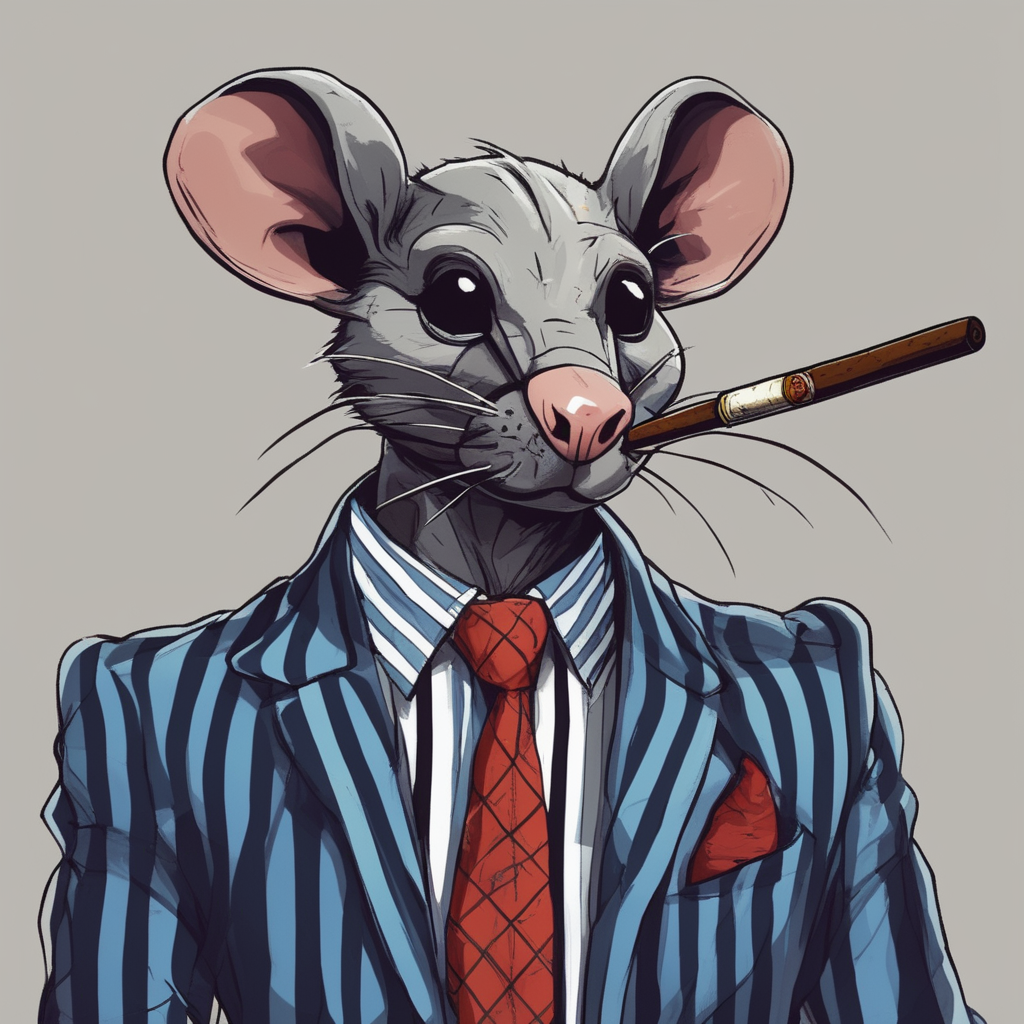
\includegraphics{create-an-image-of-a-human-folk-a-fantasy-race-with-humankind-features-resembling-a-rat-he-has-a-st-2.png}
\caption{Classica foto di Girolamo che compare alla fine degli articoli
che firma}
\end{figure}

Classica foto di Girolamo che compare alla fine degli articoli che firma

\section{Hakram}\label{hakram}

Tags: NPC Creatore: Lorenzo Ispirazione: Hart Marjok, ovviamente.

akram

\section{Hakram}\label{hakram-1}

\begin{center}\rule{0.5\linewidth}{0.5pt}\end{center}

\begin{figure}
\centering
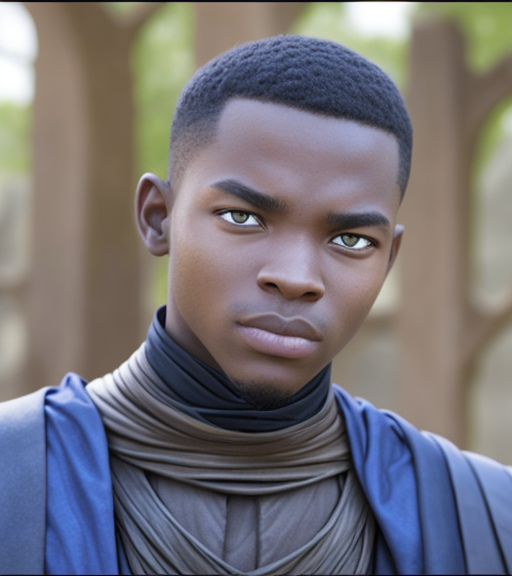
\includegraphics{a-skilled--assassin-ready-to-disappear-with-his-invisibility-cloak-he-is-a-young-black-man-he-is-a_(1).png}
\caption{a-skilled--assassin-ready-to-disappear-with-his-invisibility-cloak-he-is-a-young-black-man-he-is-a
(1).png}
\end{figure}

Informazioni Generali

Età: 27

Data di nascita: 1997

Luogo di nascita: Foresta dei Giganti

Razza: Mezz'elfo

Classe: Ladro

Alleati:

Nemesi: Impero Dishartiano

Alias:

Professione: Ladro

\begin{center}\rule{0.5\linewidth}{0.5pt}\end{center}

\subsection{1. Descrizione Generale}\label{descrizione-generale}

\begin{center}\rule{0.5\linewidth}{0.5pt}\end{center}

\begin{figure}
\centering
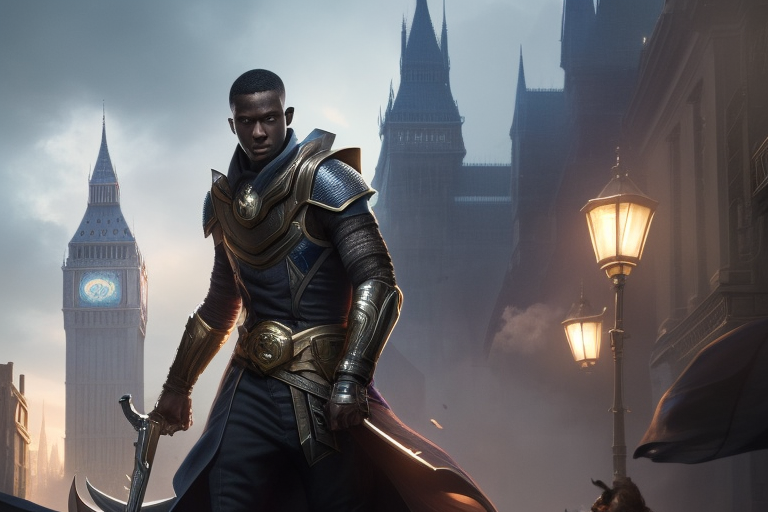
\includegraphics{a-skilled--assassin-ready-to-disappear-with-his-invisibility-cloak-he-is-a-young-black-man-he-is-a.png}
\caption{a-skilled--assassin-ready-to-disappear-with-his-invisibility-cloak-he-is-a-young-black-man-he-is-a.png}
\end{figure}

Hakram è un affascinante mezz'elfo con occhi vivaci, pelle e capelli
scuri. La sua agilità naturale è evidente in ogni movimento, e la sua
postura è sempre rilassata, pronto a sfuggire a qualsiasi situazione
pericolosa.

\subsection{2. Biografia}\label{biografia}

\begin{center}\rule{0.5\linewidth}{0.5pt}\end{center}

Cresciuto tra gli alberi dell'oscura Foresta dei Giganti da un vecchio
nano, Hakram non ha mai conosciuto i suoi genitori biologici. Dopo la
morte di suo padre adottivo, avvenuta quando aveva solo 14 anni, ha
imparato rapidamente le arti dell'inganno, del furto e della fuga,
diventando un abile ladro, girovago tra i villaggi e le città di
Valtara. Nonostante la sua vita criminale, ha un codice morale che gli
impedisce di fare del male a chi non se lo merita. Al momento nessuno sa
dove siano Hakram e Leona, ne se siano ancora vivi.

\subsection{3. Carriera}\label{carriera}

\begin{center}\rule{0.5\linewidth}{0.5pt}\end{center}

Dopo anni a vagare senza meta, Hakram si è stabilito nella capitale
Dishartiana, dove è diventato uno dei ladri più famosi per le sue
abilità di scasso e infiltrazione. È noto per i suoi colpi audaci e
sfuggenti, che gli hanno guadagnato rispetto tra i suoi compagni
criminali. La sua conoscenza dei luoghi e delle vie nascoste della
capitale dishartana è insuperabile, il che lo rende un compagno
inestimabile per qualsiasi colpo. L'imperatore ha messo sulla sua testa
una taglia di 10000 monete d'oro.

\subsection{4. Personalità}\label{personalituxe0}

\begin{center}\rule{0.5\linewidth}{0.5pt}\end{center}

Nonostante la sua professione, Hakram è un individuo affabile e
simpatico. Ha un senso dell'umorismo tagliente e sa come tranquillizzare
gli altri con la sua presenza rassicurante. È un romantico e ha un lato
gentile che riserva solo a coloro che hanno guadagnato la sua fiducia.
L'incontro con la principessa Leona ha trasformato la sua vita. Si è
innamorato profondamente di lei, e ora, con la notizia della prossima
paternità, è determinato a proteggere la principessa e il loro bambino
da qualsiasi minaccia che si profili all'orizzonte, in particolar modo
dalle responsabilità della corona. La sua abilità nel mondo dei ladri e
il suo sentimento d'amore lo hanno reso un partner devoto e pronto a
tutto.

\subsection{A. Coinvolgimenti in Eventi
Recenti}\label{a.-coinvolgimenti-in-eventi-recenti}

\begin{center}\rule{0.5\linewidth}{0.5pt}\end{center}

\href{Untitled\%20Database\%2049897c1ada034aeebc6c1efae06d3b26.csv}{Untitled
Database}

\section{Leona Narendra Pahaton}\label{leona-narendra-pahaton}

Tags: NPC Creatore: Lorenzo Luogo: Disharta

\section{\texorpdfstring{\textbf{Leona Narendra
Pahaton}}{Leona Narendra Pahaton}}\label{leona-narendra-pahaton-1}

\begin{center}\rule{0.5\linewidth}{0.5pt}\end{center}

\begin{figure}
\centering
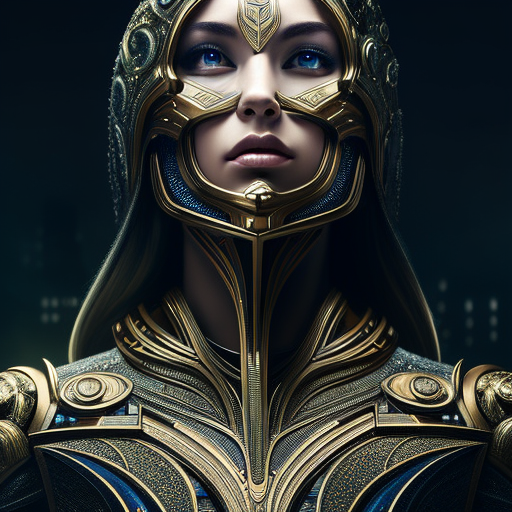
\includegraphics{Principessa_Leona.png}
\caption{Principessa Leona.png}
\end{figure}

Informazioni Generali

Età: 18

Data di nascita: 2005

Luogo di nascita: Goldendor, Disharta

Razza: Umana

Classe:

Alleati:

Nemesi:

Alias:

Professione:

\begin{center}\rule{0.5\linewidth}{0.5pt}\end{center}

\subsection{1. Descrizione Generale}\label{descrizione-generale}

\begin{center}\rule{0.5\linewidth}{0.5pt}\end{center}

\includegraphics{10}\_RITRATTO\_3.png)

La Principessa Leona di Disharta è una figura notevole all'interno del
regno, con una bellezza e grazia che catturano l'attenzione di chiunque
la incontri. ``La sua presenza è maestosa, con capelli dorati che cadono
fluidi sulle spalle e occhi azzurri come il cielo sereno sopra il suo
regno. La sua pelle è chiara, impreziosita da un tocco di rosa sulle
guance, e ha una statura slanciata che riflette l'eleganza della sua
figura regale''. È così che le principesse Dishartane vengono descritte
da sempre, anche se con capelli corti e mori, con gli occhi scuri, basse
e con la pelle color oliva, ovvero come Leona.

\subsection{2. Biografia}\label{biografia}

\begin{center}\rule{0.5\linewidth}{0.5pt}\end{center}

Unica figlia dell'Imperatore Lucius III di Disharta, la vita di Leona è
stata segnata sin dalla nascita da aspettative reali. Crescendo
all'interno delle mura del maestoso palazzo reale, è stata educata nelle
arti della politica e della diplomazia fin dalla giovane età. La sua
infanzia è stata caratterizzata da un profondo senso di dovere nei
confronti del suo popolo e dell'impero. La sua determinazione a non
sottomettersi alle rigide convenzioni dell'impero ha raggiunto l'apice
nel giorno del suo diciottesimo compleanno, quando è fuggita dal palazzo
reale alla vigilia di un matrimonio combinato. Questa scelta coraggiosa
l'ha portata lontano dal suo mondo conosciuto e ha gettato Disharta
nell'incertezza sulla successione. Al momento nessuno sa dove siano
Hakram e Leona, ne se siano ancora vivi.

\subsection{3. Carriera}\label{carriera}

\begin{center}\rule{0.5\linewidth}{0.5pt}\end{center}

Nonostante non abbia mai intrapreso una carriera tradizionale, la sua
fuga ha messo in moto una serie di eventi che influenzano profondamente
e negativamente il destino dell'Impero di Disharta. La sua vita è
diventata una lotta per la sua libertà e indipendenza.

\subsection{4. Personalità}\label{personalituxe0}

\begin{center}\rule{0.5\linewidth}{0.5pt}\end{center}

Leona è cocciuta ma coraggiosa, risoluta nel perseguire i propri
obiettivi, anche a costo di sfidare le convenzioni sociali e politiche.
Amante accanita della lettura e della geografia, trascorre le sue ore
libere immersa in libri che la portano in mondi lontani e sconosciuti. È
un'esperta conoscitrice dei territori di Valtara, anche se le sue
esplorazioni sono limitate all'immaginazione a causa della sua
situazione. Inoltre, il suo cuore è stato rubato da un ladro girovago
che ha incontrato durante una delle sue tante fughe notturne. Il loro
amore è stato rapido ma intenso, e Leona è rimasta incinta di lui.
Questa nuova prospettiva di maternità ha aggiunto ulteriore
determinazione alla sua lotta per la libertà e l'indipendenza, poiché
vuole garantire un futuro migliore per il suo bambino, lontano dagli
obblighi dell'impero Dishartiano.

\subsection{A. Coinvolgimenti in Eventi
Recenti}\label{a.-coinvolgimenti-in-eventi-recenti}

\begin{center}\rule{0.5\linewidth}{0.5pt}\end{center}

\href{Untitled\%20Database\%203437f651bc3346468e1534d3b16d20e1.csv}{Untitled
Database}

\section{Lucius III di Dishartha (Lucius Narendra
Pahaton)}\label{lucius-iii-di-dishartha-lucius-narendra-pahaton}

Tags: NPC Creatore: Lorenzo Luogo: Disharta, Goldendoor

\section{\texorpdfstring{\textbf{Lucius Narendra
Pahaton}}{Lucius Narendra Pahaton}}\label{lucius-narendra-pahaton}

\begin{center}\rule{0.5\linewidth}{0.5pt}\end{center}

\begin{figure}
\centering
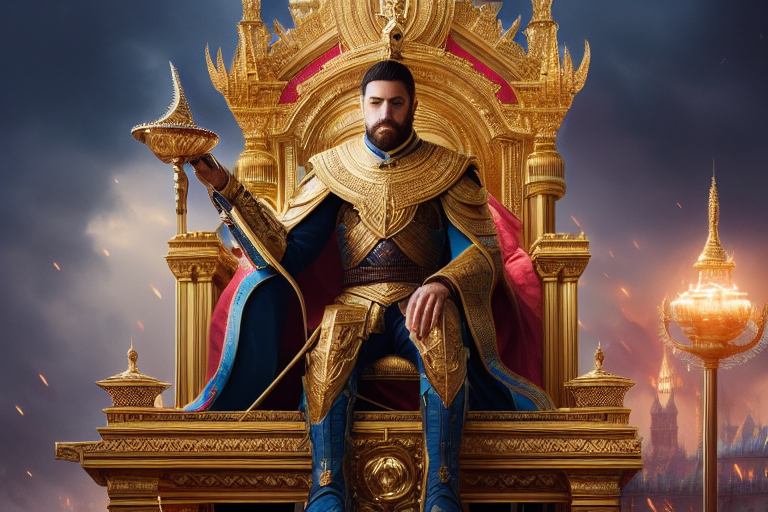
\includegraphics{01_IMPERATORE.png}
\caption{01\_IMPERATORE.png}
\end{figure}

Informazioni Generali

Età: 58

Data di nascita: 1996

Luogo di nascita: Goldendoor

Razza: Umano

Classe:

Alleati:

Nemesi:

Alias:

Professione: Imperatore di Disharta

\begin{center}\rule{0.5\linewidth}{0.5pt}\end{center}

\subsection{1. Descrizione Generale}\label{descrizione-generale}

\begin{center}\rule{0.5\linewidth}{0.5pt}\end{center}

\begin{figure}
\centering
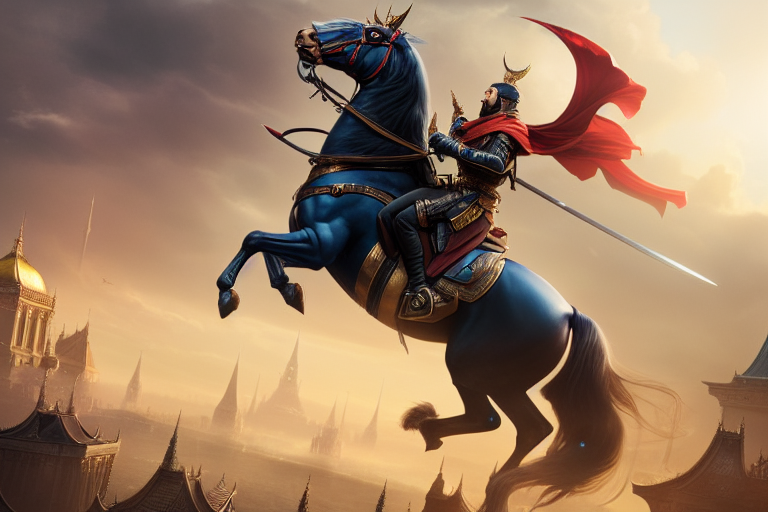
\includegraphics{emperor-on-his-trhone-trending-on-artstation-sharp-focus-studio-photo-intricate-details-highly-.png}
\caption{emperor-on-his-trhone-trending-on-artstation-sharp-focus-studio-photo-intricate-details-highly-.png}
\end{figure}

L'Imperatore Lucius III di Disharta è un uomo imponente con un
portamento regale. Ha capelli neriben pettinati e un viso severo con
occhi penetranti che riflettono la sua autorità. Indossa abiti sontuosi
e una corona d'oro che simboleggia la sua posizione di supremo sovrano.

\subsection{2. Biografia}\label{biografia}

\begin{center}\rule{0.5\linewidth}{0.5pt}\end{center}

Lucius III è nato nella famiglia reale di Disharta ed è cresciuto con
l'idea che un giorno avrebbe dovuto regnare sull'impero. È stato educato
nei principi della leadership, della politica e della strategia militare
fin dalla giovinezza. Ha salito i gradini della gerarchia reale fino a
diventare imperatore.

\subsection{3. Carriera}\label{carriera}

\begin{center}\rule{0.5\linewidth}{0.5pt}\end{center}

La carriera di Lucius III è stata dedicata al governo e alla gestione
dell'Impero di Disharta. Ha dimostrato di essere un sovrano abile,
maestro della diplomazia e dell'arte della politica. Ha guidato l'impero
attraverso periodi di prosperità e crisi, mantenendo la sua autorità
incondizionata. La sua preoccupazione principale è stata sempre
garantire la stabilità e la crescita dell'impero.

\subsection{4. Personalità}\label{personalituxe0}

\begin{center}\rule{0.5\linewidth}{0.5pt}\end{center}

L'Imperatore Lucius III è un uomo di ambizione ardente e determinazione
ferrea. Col passare degli anni, il suo unico desiderio è diventato
quello di assicurare la continuità del suo lignaggio e l'ascesa di un
erede maschio al trono di Disharta. Alla nascita della principessa Leona
il suo cuore è rimasto freddo, poiché la sua ambizione era rivolta a un
erede maschio. L'imperatore è noto per la sua freddezza e indifferenza
verso la figlia. Ha speso gran parte della vita della figlia a cercare
di forgiare alleanze matrimoniali per consolidare il suo potere,
ignorando le esigenze emotive di Leona. La sua decisione di cercare di
farla tornare al palazzo dopo la sua fuga è dettata più dalla
preoccupazione per la stabilità dell'impero che dall'affetto paterno.

\subsection{A. Coinvolgimenti in Eventi
Recenti}\label{a.-coinvolgimenti-in-eventi-recenti}

\begin{center}\rule{0.5\linewidth}{0.5pt}\end{center}

\href{Untitled\%20Database\%20665a498987254279b64261b8cc19c10e.csv}{Untitled
Database}

\section{Marpalo Rem}\label{marpalo-rem}

Tags: NPC, Quartiermastro Alias: Il Divoratore Pacato Creatore: Davide
Ispirazione: Omar Palermo Razza: Umano Classe: Paladino

\section{Marpalo Rem}\label{marpalo-rem-1}

\begin{center}\rule{0.5\linewidth}{0.5pt}\end{center}

\begin{figure}
\centering
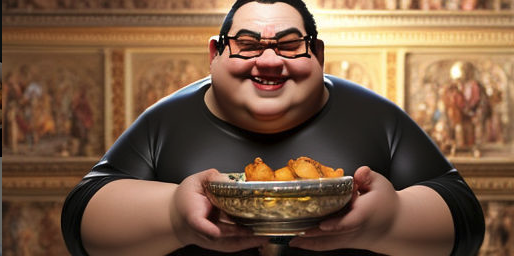
\includegraphics{Screen_Shot_2023-04-06_at_00.57.24_AM.png}
\caption{Screen Shot 2023-04-06 at 00.57.24 AM.png}
\end{figure}

Informazioni Generali

Età: 42

Anno di nascita:

Paese di nascita: Kos

Razza: Umano

Relazioni:

Alleati: Gilda dei Protettori; Ordine dei Paladini di San Francesco;
Cibo.

Nemesi:

Possedimenti importanti: 200 kg di panza

Professione: Quartiermastro

\begin{center}\rule{0.5\linewidth}{0.5pt}\end{center}

\subsection{1. Descrizione Generale}\label{descrizione-generale}

\begin{center}\rule{0.5\linewidth}{0.5pt}\end{center}

Marpalo Rem, il Quartiermastro della Gilda dei Protettori di Kos, è un
affascinante personaggio umano con un fisico imponente. La sua
corporatura è robusta e obesa, con una pancia pronunciata che sembra
sempre pronta a scodellare un nuovo pasto. Nonostante la sua forma
fisica non sia esattamente quella di un avventuriero in forma
smagliante, Marpalo ha un sorriso contagioso e uno sguardo vivace nei
suoi occhi castani. Marpalo indossa sempre un elegante abito da
quartiermastro, che ha un sacco di tasche per tenere i suoi numerosi
strumenti e documenti.

\begin{quote}
``Buonasera, cari confratelli protettori''
\end{quote}

\subsection{2. Biografia}\label{biografia}

\begin{center}\rule{0.5\linewidth}{0.5pt}\end{center}

Nato e cresciuto nella città di Kos, Marpalo ha avuto un'infanzia umile
ma felice. Fin da piccolo, sviluppò una passione per il cibo, sempre
desideroso di scoprire nuovi sapori e provare piatti deliziosi.
Tuttavia, la sua passione lo portò a un aumento di peso significativo,
ma questo non lo scoraggiò affatto. Marpalo trovò conforto
nell'apprendimento e nella lettura, trascorrendo ore nella biblioteca
cittadina a studiare ogni tipo di argomento, dalla storia alle arti
arcane.

Con il passare degli anni, Marpalo divenne un esperto conoscitore della
storia di Kos e delle terre circostanti. Quando i Protettori di Kos, una
rinomata gilda di avventurieri, aprirono le porte per reclutare nuovi
membri, Marpalo vide un'opportunità unica per mettere a frutto la sua
conoscenza e la sua passione per l'avventura.

\subsection{3. Carriera}\label{carriera}

\begin{center}\rule{0.5\linewidth}{0.5pt}\end{center}

Marpalo si unì ai Protettori di Kos come quartiermastro, un ruolo che
gli consentiva di mettere in mostra le sue abilità organizzative e le
sue conoscenze storiche. Come quartiermastro, è responsabile della
gestione delle forniture, dell'equipaggiamento e degli
approvvigionamenti della gilda. Marpalo ha dedicato molto tempo e sforzo
a costruire una rete di contatti in tutta la regione, assicurandosi che
i Protettori di Kos abbiano sempre accesso alle risorse di cui hanno
bisogno per le loro imprese.

Oltre a occuparsi dell'aspetto logistico, Marpalo si è anche impegnato a
condividere la sua vasta conoscenza con i membri della gilda. Organizza
frequenti lezioni e conferenze sulla storia, la cultura e le arti
magiche, cercando di arricchire le menti degli avventurieri e di
incoraggiarli a comprendere il mondo che li circonda.

\begin{quote}
``Oggi andremo ad assegnarvi questa missione''
\end{quote}

\subsection{4. Personalità}\label{personalituxe0}

\begin{center}\rule{0.5\linewidth}{0.5pt}\end{center}

Marpalo Rem è noto per essere affabile e amichevole. Nonostante la sua
corporatura obesa e la calvizie, è un uomo estremamente fiducioso e
felice di sé. La sua presenza è contagiosa e riesce a mettere a proprio
agio chiunque entri in contatto con lui.

Marpalo è un vero intenditore del cibo e ama condividere questa passione
con gli altri. Organizza frequentemente sfide mangerecce con gli
avventurieri della gilda, spingendosi al limite per testare la sua
resistenza gastronomica.

Nonostante la sua natura amichevole, Marpalo non tollera chi lo
contraddice. È deciso nelle sue opinioni e può essere testardo quando si
tratta di questioni di gilda. La sua vasta conoscenza storica e
culturale lo rende un punto di riferimento per i membri della gilda, che
spesso si rivolgono a lui per consigli e indicazioni.

\subsection{A. Coinvolgimenti in eventi
recenti}\label{a.-coinvolgimenti-in-eventi-recenti}

\begin{center}\rule{0.5\linewidth}{0.5pt}\end{center}

\href{Untitled\%20Database\%20a55e9319918d439c8e425a299be97c3d.csv}{Untitled
Database}

\subsection{B. Aggiornamenti}\label{b.-aggiornamenti}

\begin{center}\rule{0.5\linewidth}{0.5pt}\end{center}

\href{Untitled\%20c80f6936cdaf4d19b2c69d1f3802947e.csv}{}

\section{Nicolos}\label{nicolos}

Tags: NPC Creatore: Lorenzo Ispirazione: Athelstan (Vikings)

\section{Nicolos}\label{nicolos-1}

\begin{center}\rule{0.5\linewidth}{0.5pt}\end{center}

\begin{figure}
\centering
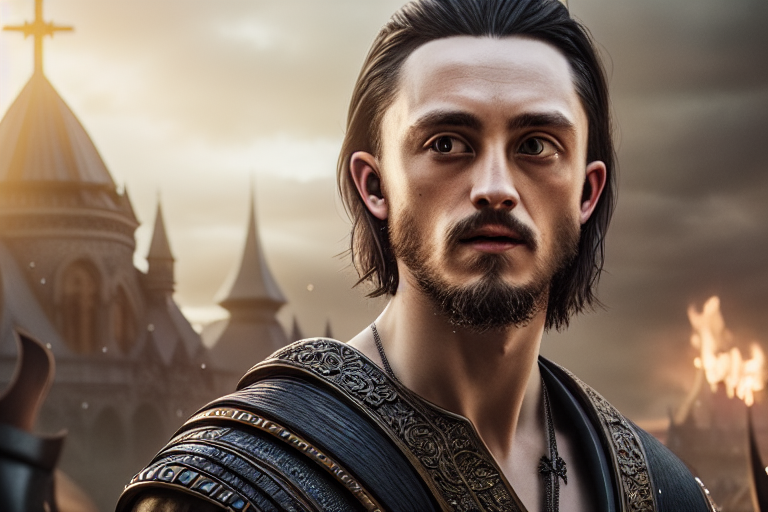
\includegraphics{athelstan-from-vikings-perfect-composition-beautiful-detailed-intricate-insanely-detailed-octane-r.png}
\caption{athelstan-from-vikings-perfect-composition-beautiful-detailed-intricate-insanely-detailed-octane-r.png}
\end{figure}

Informazioni Generali

Età: 38

Anno di nascita: 1985

Paese di nascita: Pandosia

Razza: Umano

Relazioni:

Alleati:

Nemesi:

Possedimenti importanti:

Professione: Sacerdote del Tempio di San Nicolos Dibar

\begin{center}\rule{0.5\linewidth}{0.5pt}\end{center}

\subsection{1. Descrizione Generale}\label{descrizione-generale}

\begin{center}\rule{0.5\linewidth}{0.5pt}\end{center}

Il \textbf{Sacerdote Nicolos} è una figura rispettata e ammirata nella
città di @pandosia, noto per la sua dedizione al tempio di San Nicolos
di Bar.

\begin{quote}
Donare riempie il cuore di chi dona e di chi riceve, proprio come
insegna San Nicolos Dibar
\end{quote}

\subsection{2. Biografia}\label{biografia}

\begin{center}\rule{0.5\linewidth}{0.5pt}\end{center}

Nicolos è nato a Pandosia nel 1985, in una famiglia profondamente
devota. Fin dalla giovane età, dimostrò una profonda connessione con gli
insegnamenti di San Nicolos di Bar, il patrono della città. Dopo
un'infanzia segnata da un profondo senso di fede e spiritualità, Nicolos
decise di dedicare la sua vita al servizio divino.

\subsection{3. Carriera}\label{carriera}

\begin{center}\rule{0.5\linewidth}{0.5pt}\end{center}

Il Tempio di San Nicolos di Bar è uno dei luoghi di culto più antichi e
venerati di Pandosia, noto per la sua architettura maestosa e la sua
storia ricca di tradizione. Nicolos intraprese il suo percorso
spirituale diventando un sacerdote del tempio, e il suo impegno fu
presto riconosciuto dalla comunità.

Nicolos divenne rapidamente noto per la sua saggezza e compassione.
Oltre a officiare le cerimonie religiose e guidare i riti sacri del
tempio, dedicò gran parte del suo tempo a consolare i bisognosi,
ascoltare i problemi dei fedeli e offrire saggi consigli. La sua
capacità di mettersi in relazione con le persone e di alleviare il loro
dolore gli guadagnò una reputazione di guida spirituale straordinaria.

Nicolos si distinse anche per il suo impegno comunitario. Organizzava
regolarmente eventi di beneficenza per raccogliere fondi per gli orfani,
i malati e i meno fortunati, seguendo l'esempio di San Nicolos di Bar,
noto per la sua generosità. Questi sforzi consolidarono ulteriormente il
suo status come un faro di speranza e aiuto nella città di Pandosia.

\subsection{4. Personalità}\label{personalituxe0}

\begin{center}\rule{0.5\linewidth}{0.5pt}\end{center}

\subsection{5. Coinvolgimenti in eventi
recenti}\label{coinvolgimenti-in-eventi-recenti}

\begin{center}\rule{0.5\linewidth}{0.5pt}\end{center}

\href{Untitled\%20Database\%206862812dd1bd4510960e013bb45ddbf8.csv}{Untitled
Database}

\subsection{6. Scheda personaggio}\label{scheda-personaggio}

\begin{center}\rule{0.5\linewidth}{0.5pt}\end{center}

\href{Info\%20PG\%204df6886f9e2044c494002856a4ea0f50.csv}{Info PG}

\subsubsection{Statistiche e abilità}\label{statistiche-e-abilituxe0}

\begin{center}\rule{0.5\linewidth}{0.5pt}\end{center}

\href{Abilita\%CC\%80\%20e49d5669224e41728d04dce2a31d4614.csv}{Abilità}

\subsubsection{Lista magie}\label{lista-magie}

\subsection{A. Descrizione originale}\label{a.-descrizione-originale}

\begin{center}\rule{0.5\linewidth}{0.5pt}\end{center}

\section{Rhyderch Hayenne}\label{rhyderch-hayenne}

Tags: NPC Creatore: Davide Luogo: Azura

\section{Rhyderch Hayenne}\label{rhyderch-hayenne-1}

\begin{center}\rule{0.5\linewidth}{0.5pt}\end{center}

\begin{figure}
\centering
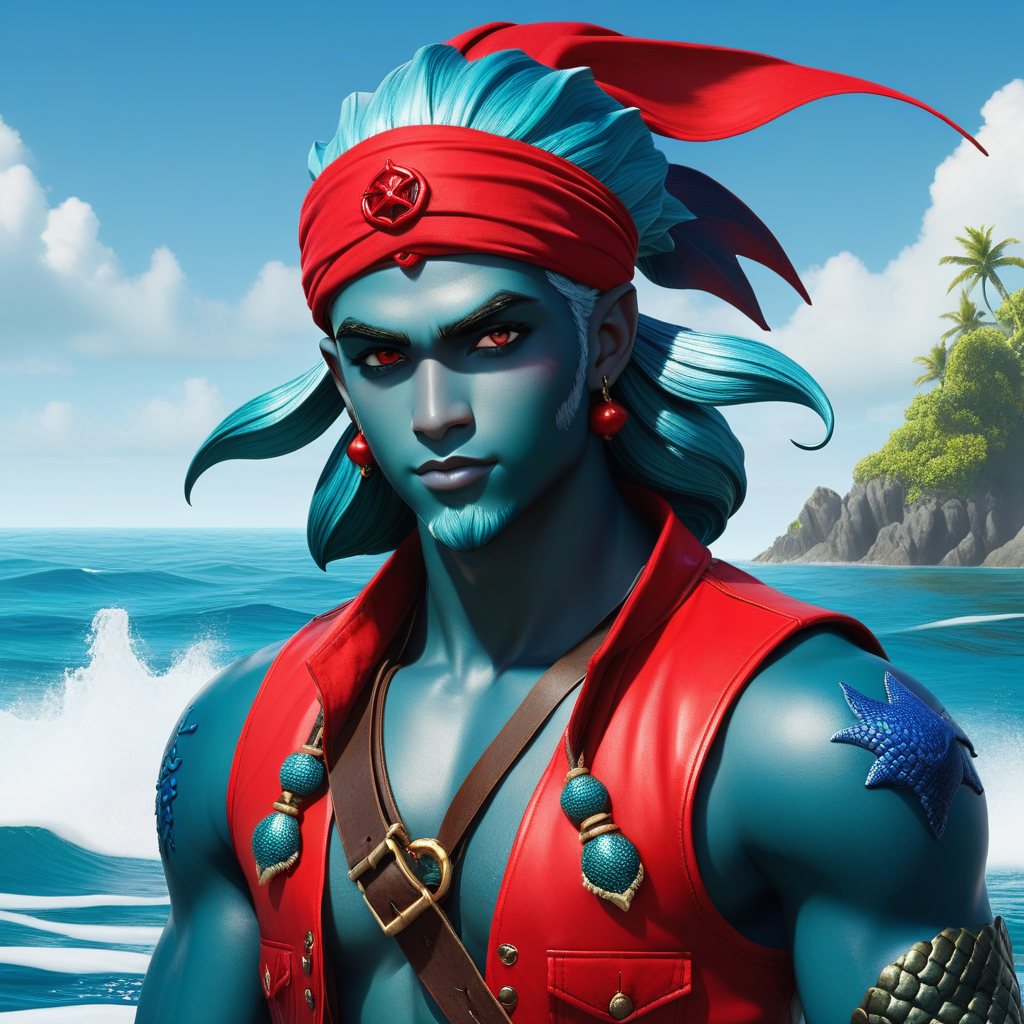
\includegraphics{generate-an-image-of-a-merfolk-named-rhyderch-hayenne-he-has-vibrant-blue-skin-wears-a-red-bandana-2.png}
\caption{generate-an-image-of-a-merfolk-named-rhyderch-hayenne-he-has-vibrant-blue-skin-wears-a-red-bandana-2.png}
\end{figure}

Informazioni Generali

Età:

Data di nascita:

Luogo di nascita:

Razza: Merfolk

Classe: Guerriero

Alleati:

Nemesi: I Pirati

Alias:

Professione: Marinaio

\begin{center}\rule{0.5\linewidth}{0.5pt}\end{center}

\subsection{1. Descrizione Generale}\label{descrizione-generale}

\begin{center}\rule{0.5\linewidth}{0.5pt}\end{center}

\begin{figure}
\centering
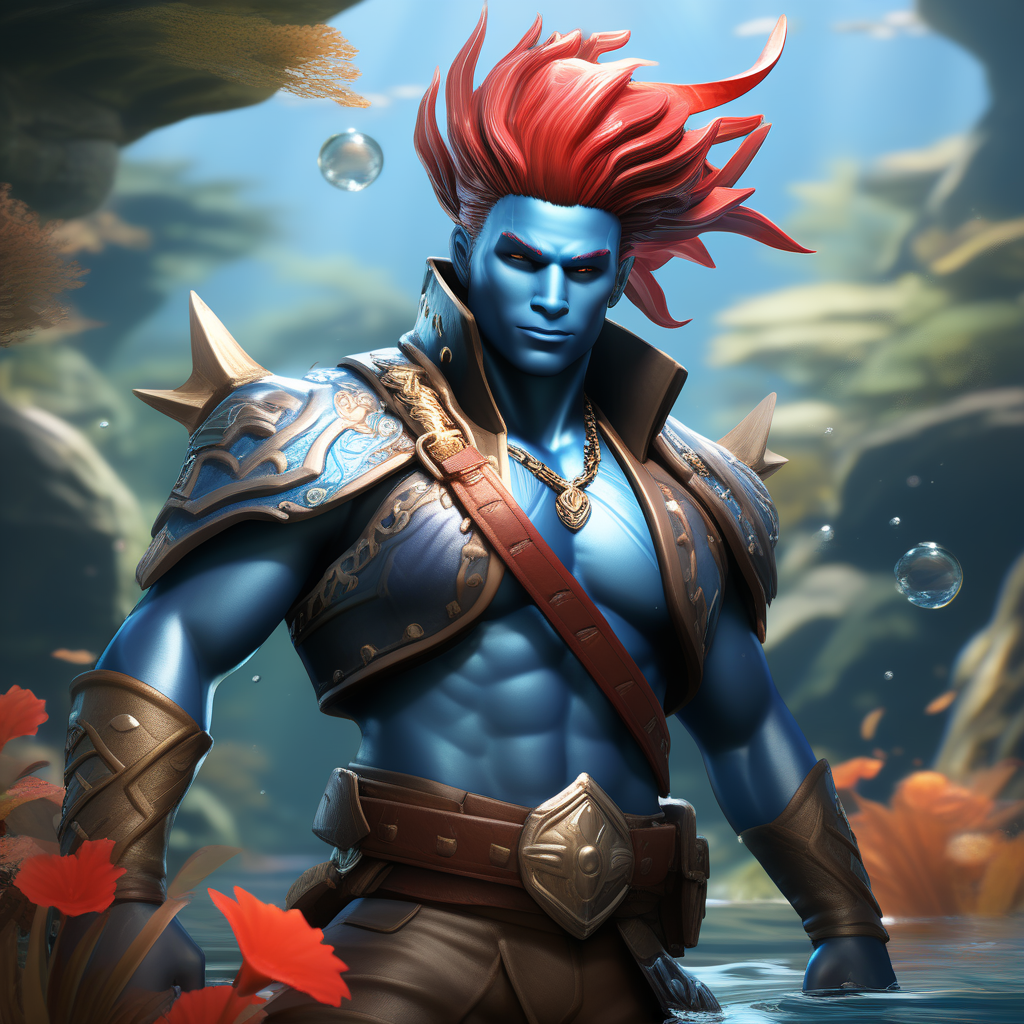
\includegraphics{generate-an-image-of-a-merfolk-named-rhyderch-hayenne-he-has-vibrant-blue-skin-wears-a-red-bandana.png}
\caption{generate-an-image-of-a-merfolk-named-rhyderch-hayenne-he-has-vibrant-blue-skin-wears-a-red-bandana.png}
\end{figure}

Rhyderch Hayenne è un merfolk nato e cresciuto nelle acque scintillanti
di Azura. Con una fisicità snodabile e scaglie che riflettono i colori
del mare, Rhyderch è un esempio vivente della grazia e della forza del
suo popolo. Tuttavia, dietro i suoi occhi intensi e la postura regale,
si nasconde una storia di sofferenza e determinazione.

La sua lingua, una volta eloquente, è stata crudelmente strappata
durante i giorni di prigionia tra le grinfie di pirati senza scrupoli.
Ciò ha donato al suo sguardo un'aura di profonda risolutezza, mentre le
cicatrici sulle sue scaglie raccontano la storia di un merfolk che ha
attraversato le acque tempestose della vita

\begin{quote}
``\ldots{}''
\end{quote}

\subsection{2. Biografia}\label{biografia}

\begin{center}\rule{0.5\linewidth}{0.5pt}\end{center}

\subsubsection{\texorpdfstring{2.1
\textbf{Infanzia}}{2.1 Infanzia}}\label{infanzia}

Rhyderch è nato in una comunità di marinai a Azura, figlio di genitori
appassionati del mare. Fin dalla più tenera età, è stato affascinato
dalle leggende oceaniche e ha imparato l'arte della navigazione e
dell'esplorazione. La sua infanzia è stata caratterizzata da giornate
passate a nuotare tra coralli luminosi e a giocare con gli altri giovani
merfolk, sognando di un giorno solcare i mari come i marinai delle
storie raccontate dai genitori.

\subsubsection{\texorpdfstring{2.2
\textbf{Gioventù}}{2.2 Gioventù}}\label{gioventuxf9}

Con l'avanzare degli anni, Rhyderch ha iniziato a esplorare i porti di
Valtara, stringendo legami con diverse comunità costiere. La sua
gioventù è stata segnata da avventure entusiasmanti e incontri con
creature marine affascinanti. Tuttavia, la sua vita ha subito una svolta
tragica quando è caduto prigioniero di pirati brutali durante uno dei
suoi viaggi.

\subsubsection{\texorpdfstring{2.3 \textbf{Vita
Adulta}}{2.3 Vita Adulta}}\label{vita-adulta}

Dopo giorni di prigionia e tormento, Rhyderch è riuscito a fuggire, ma
il prezzo pagato è stato alto. La sua lingua è stata strappata via,
privandolo della voce che una volta riempiva il mare di canti e
racconti. Rientrato ad Azura, ha cercato rifugio nella Gilda dei
Protettori, unendosi a loro con l'ardente desiderio di impedire che
altri subiscano la stessa sorte.

La sua vita adulta è divenuta un'ode alla determinazione. Rhyderch ha
affrontato le sfide del suo passato, trasformandosi in un difensore
inflessibile del mare. All'interno della Gilda dei Protettori, ha
canalizzato la sua esperienza personale nella caccia ai pirati,
divenendo uno dei principali marinai, rispettato per la sua abilità di
navigazione e la sua ferocia nel combattimento.

Ogni azione di Rhyderch è permeata dalla sua dedizione a proteggere gli
innocenti e a preservare la tranquillità nelle acque di Valtara. La sua
storia è un inno alla resilienza e alla forza che si può trovare anche
nelle profondità più oscure del mare.

\subsection{3. Carriera}\label{carriera}

\begin{center}\rule{0.5\linewidth}{0.5pt}\end{center}

Prima di unirsi alla Gilda, Rhyderch aveva già guadagnato fama tra i
marinai per le sue abilità di navigazione e il suo coraggio nelle
situazioni pericolose. Tuttavia, la sua transizione da marinaio
indipendente a membro della Gilda dei Protettori è stata un passo
significativo nella sua carriera.

All'interno della Gilda, Rhyderch ha affinato le sue abilità di
combattimento e strategia, diventando uno dei principali marinai
dedicati alla caccia ai pirati. La sua storia personale di sofferenza e
sopravvivenza si è trasformata in una forza motivante per proteggere gli
innocenti e preservare la pace nelle acque di Valtara.

Ogni impegno di Rhyderch è un tributo alla resilienza e alla volontà di
superare le avversità. Il suo nome è diventato sinonimo di speranza e
protezione tra le comunità costiere, un faro di luce nei mari spesso
oscuri del mondo.

\subsection{4. Personalità}\label{personalituxe0}

\begin{center}\rule{0.5\linewidth}{0.5pt}\end{center}

La personalità di Rhyderch è un intricato intreccio di determinazione e
compassione. La sua esperienza di vita ha forgiato un individuo
risoluto, deciso a difendere gli oppressi e a combattere le ingiustizie
dei mari. Nonostante la perdita della lingua, la sua comunicazione non
verbale è eloquente, esprimendo empatia e solidarietà verso coloro che
hanno sofferto.

Nelle situazioni sociali, Rhyderch è attento e riflessivo, ascoltando
con attenzione anche senza l'uso delle parole. La sua presenza
tranquilla trasmette sicurezza, e la sua risolutezza nelle decisioni è
evidente sia in battaglia che nei momenti di pace. Il suo senso
dell'onore e della giustizia lo guida attraverso le sfide, facendolo
emergere come un leader rispettato tra i membri della Gilda dei
Protettori.

\subsection{A. Coinvolgimenti in Eventi
Recenti}\label{a.-coinvolgimenti-in-eventi-recenti}

\begin{center}\rule{0.5\linewidth}{0.5pt}\end{center}

\href{Untitled\%20Database\%20895b8280d00349d8b81d32eab032133f.csv}{Untitled
Database}

\subsection{B. Aggiornamenti}\label{b.-aggiornamenti}

\begin{center}\rule{0.5\linewidth}{0.5pt}\end{center}

\href{Untitled\%20c4a53933cd0a4b9dbbead926bfd528d4.csv}{}

\section{Sam Windrider}\label{sam-windrider}

Tags: NPC, Quartiermastro Creatore: Lorenzo

\section{Sam Windrider}\label{sam-windrider-1}

\begin{center}\rule{0.5\linewidth}{0.5pt}\end{center}

\begin{figure}
\centering
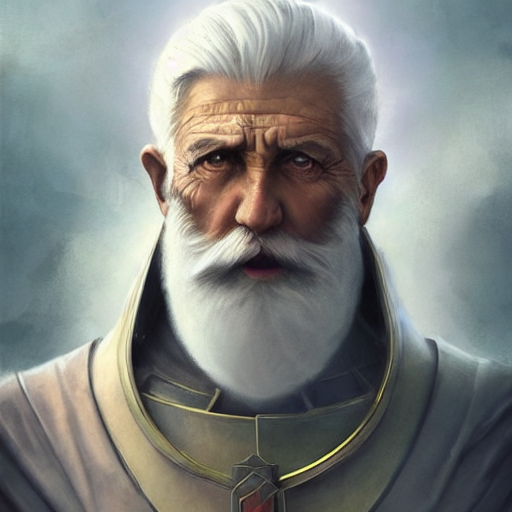
\includegraphics{Sam_Windrider.png}
\caption{Sam Windrider.png}
\end{figure}

Informazioni Generali

Età: 78

Anno di nascita: 1945

Paese di nascita: Kos

Razza: Umano

Relazioni:

Alleati: Gilda dei Protettori, Ordine dei Paladini di San Francesco.

Nemesi: Setta del Sangue

Possedimenti importanti:

Ruolo: Gran Custode del Tempio

\begin{center}\rule{0.5\linewidth}{0.5pt}\end{center}

\subsection{1. Descrizione Generale}\label{descrizione-generale}

\begin{center}\rule{0.5\linewidth}{0.5pt}\end{center}

Sam ha ancora un portamento fiero, nonostante la sua età avanzata. La
sua postura è leggermente curva, ma ciò non diminuisce la sua presenza
imponente. Il suo viso rugoso e segnato dal tempo è illuminato da un
sorriso gentile, mentre i suoi occhi incavati e profondi sembrano
raccontare tutto il dolore che hanno visto nella loro lunga vita.
Nonostante l'età avanzata, cammina con passo fermo e ha occhi brillanti
di saggezza. Dopo la morte del figlio, Sam decise di deporre le armi e
di ritirarsi nel tempio di San Francesco. Non volendo più essere
coinvolto nella violenza del mondo esterno, dedicò il resto della sua
vita alla preghiera e alla meditazione. È il paladino capo del tempio di
San Francesco ed è sua premura occuparsi di ogni cosa: dal benessere dei
fedeli alla manutenzione della struttura. La sua presenza ispira
rispetto e calma a tutti coloro che si avvicinano a lui, e la sua
saggezza è ricercata da molti che cercano consiglio e conforto.

\subsection{2. Biografia}\label{biografia}

\begin{center}\rule{0.5\linewidth}{0.5pt}\end{center}

\subsection{3. Carriera}\label{carriera}

\begin{center}\rule{0.5\linewidth}{0.5pt}\end{center}

\subsection{4. Personalità}\label{personalituxe0}

\begin{center}\rule{0.5\linewidth}{0.5pt}\end{center}

\subsection{A. Coinvolgimenti in eventi
recenti}\label{a.-coinvolgimenti-in-eventi-recenti}

\begin{center}\rule{0.5\linewidth}{0.5pt}\end{center}

\href{Untitled\%20Database\%2011e31a90c4de4b4e8b6da34fd12f13e9.csv}{Untitled
Database}

\subsection{B. Aggiornamenti}\label{b.-aggiornamenti}

\begin{center}\rule{0.5\linewidth}{0.5pt}\end{center}

\href{Untitled\%20f91756bc0aea4e4ab43710d40315e574.csv}{}

\section{Silvio Berlusconi}\label{silvio-berlusconi}

Tags: NPC Alias: Il cavaliere Creatore: Lorenzo Ispirazione: Silvio
Berlusconi

\section{Silvio Berlusconi}\label{silvio-berlusconi-1}

\begin{center}\rule{0.5\linewidth}{0.5pt}\end{center}

\begin{figure}
\centering
\includegraphics{a-smiling-black-newborn_(1).png}
\caption{a-smiling-black-newborn (1).png}
\end{figure}

Informazioni Generali

Età: 1

Anno di nascita: 2023

Paese di nascita: ?

Razza: umano

Relazioni: Ultimo cadetto dei Paladini di San Francesco

Alleati: Ordine dei Paladini di San Francesco, Gilda dei Protettori

Nemesi: Naskirophis

Possedimenti importanti:

Professione:

\begin{center}\rule{0.5\linewidth}{0.5pt}\end{center}

\subsection{1. Descrizione Generale}\label{descrizione-generale}

\begin{center}\rule{0.5\linewidth}{0.5pt}\end{center}

\textbf{Silvio Berlusconi} è una figura straordinaria nel mondo degli
avventurieri e degli eroi. Nato sotto circostanze enigmatiche, è un
bambino la sua storia è un racconto avvincente di rapimento, poteri
sovraumani e profezie oscure.

\subsection{2. Biografia}\label{biografia}

\begin{center}\rule{0.5\linewidth}{0.5pt}\end{center}

Le origini di Silvio Berlusconi sono avvolte nel mistero. Non si sa dove
sia nato né chi siano i suoi genitori. La sua storia inizia con un
oscuro rapimento da parte degli accoliti della
\href{Setta\%20del\%20Sangue\%202859c4de945546eda0cee6fb151ef956.md}{Setta
del Sangue} , un culto noto per il suo legame con il demone
\href{Naskirophis\%20120e02c652b84f2abeac36fef59c28f6.md}{Naskirophis} e
per i suoi rituali sacrificali. Silvio era destinato a essere
sacrificato, ma il destino aveva altri piani.

Durante una missione dei Protettori della Gilda di
\href{Kos\%20bb2884f1df2e4e47890b8cefddb5e4bd.md}{Kos}
(\href{Il\%20neonato\%20incasinato\%2090743e94446c4f5a846f18c37fd80698.md}{Il
neonato incasinato} ) nel tempio di Naskirophis, Silvio Berlusconi
mostrò poteri sovraumani che stupirono e sconcertarono gli stessi
Protettori. La natura precisa di questi poteri rimane un enigma, ma sono
stati descritti come manifestazioni di forze e abilità divine.

Naskirophis, il demone al quale Silvio Berlusconi era destinato a essere
sacrificato, fece qualcosa di sorprendente prima di morire. Piantò un
seme oscuro nel cuore di Silvio, che segnò il suo destino in modo
indelebile. Questo gesto sconvolgente gettò le basi per una profezia
oscura che avrebbe seguito la vita di Silvio Berlusconi, indicando un
futuro incerto e terribile.

I Protettori
(\href{Disis\%20Iulukinfor\%20e7699726707a41be926c823d67941f78.md}{Disis
Iulukinfor},
\href{Dorian\%20Be\%20af030367f8054333912b2dca0de16d6f.md}{Dorian Be},
\href{Pippo\%20Francfrog\%204d15378e582d4f1db815d957fe064245.md}{Pippo
Francfrog} e
\href{Sabaku\%20no\%20Darude\%209c414f3e551144f4acee665cab478336.md}{Sabaku
no Darude}) hanno deciso di battezzarlo e di affidarlo alle cure dell'
\href{Ordine\%20dei\%20Paladini\%20di\%20San\%20Francesco\%20e8fd423783714ddeb11ec757edea519b.md}{Ordine
dei Paladini di San Francesco}. I paladini lo crescerano secondo i loro
ideali, cercando di allontanarlo dal suo tragico destino, che vede il
bambino come seconda reincarnazione del demone.

\subsection{3. Carriera}\label{carriera}

\begin{center}\rule{0.5\linewidth}{0.5pt}\end{center}

\subsection{4. Personalità}\label{personalituxe0}

\begin{center}\rule{0.5\linewidth}{0.5pt}\end{center}

\subsection{A. Coinvolgimenti in eventi
recenti}\label{a.-coinvolgimenti-in-eventi-recenti}

\begin{center}\rule{0.5\linewidth}{0.5pt}\end{center}

\href{Untitled\%20Database\%20ca9cae84324f400cab8a33943de865ba.csv}{Untitled
Database}

\subsection{B. Aggiornamenti}\label{b.-aggiornamenti}

\begin{center}\rule{0.5\linewidth}{0.5pt}\end{center}

\href{Untitled\%20c6c5b00f95474402853e4e6d21c070a6.csv}{}

\section{Simon Ricchiardo di Fagot}\label{simon-ricchiardo-di-fagot}

Tags: NPC Creatore: Lorenzo Ispirazione: Enzo Miccio Luogo: Disharta

\section{\texorpdfstring{\textbf{Simon Ricchiardo di
Fagot}}{Simon Ricchiardo di Fagot}}\label{simon-ricchiardo-di-fagot-1}

\begin{center}\rule{0.5\linewidth}{0.5pt}\end{center}

\begin{figure}
\centering
\includegraphics{02_DUCA.png}
\caption{02\_DUCA.png}
\end{figure}

Informazioni Generali

Età: 40

Data di nascita: 1984

Luogo di nascita: Fagot

Razza: Umano

Classe:

Alleati:

Nemesi:

Alias:

Professione: Duca del Fagot

\begin{center}\rule{0.5\linewidth}{0.5pt}\end{center}

\subsection{1. Descrizione Generale}\label{descrizione-generale}

\begin{center}\rule{0.5\linewidth}{0.5pt}\end{center}

Il Duca Simon Ricchiardo di Fagot è un nobile di nascita, noto per la
sua spocchia e la sua aria aristocratica. La sua presenza è spesso
accompagnata da una sensazione di superiorità, e non si sforza affatto
di nascondere il suo disprezzo per chi considera socialmente inferiore.

\begin{quote}
\emph{``Esteban, raggiungimi nei miei appartamenti tra 10 minuti\ldots{}
E vieni senza camicia!''}
\end{quote}

\subsection{2. Biografia}\label{biografia}

\begin{center}\rule{0.5\linewidth}{0.5pt}\end{center}

Simon è nato in una famiglia nobile con una lunga storia di servizio
all'Impero di Disharta. Cresciuto con una forte educazione
aristocratica, ha ricevuto un addestramento adeguato alla sua posizione
come futuro Duca del Fagot. Sin da giovane, ha dimostrato un impegno per
il benessere del suo ducato e della sua futura posizione. Diverse sono
le voci che suggeriscono che la sua sessualità possa essere al di fuori
degli schemi tradizionali, motivo per cui ha sempre rifiutato proposte
di matrimonio.

\subsection{3. Carriera}\label{carriera}

\begin{center}\rule{0.5\linewidth}{0.5pt}\end{center}

Simon ha iniziato a partecipare agli affari politici dell'Impero fin da
giovane. Ha svolto incarichi diplomatici e ha rappresentato l'Impero in
varie occasioni, guadagnandosi la reputazione di un diplomatico esperto.
La sua nomina come promesso sposo di Leona è stata vista come un
tentativo di consolidare ulteriormente l'unità dell'Impero, in quanto il
ducato del Fagot ha un peso considerevole all'interno degli equilibri
politici dell'Impero.

\subsection{4. Personalità}\label{personalituxe0}

\begin{center}\rule{0.5\linewidth}{0.5pt}\end{center}

La personalità di Simon è notoriamente spocchia e sprezzante. Si
considera superiore agli altri a causa del suo lignaggio nobiliare e
della sua ricchezza. È noto per il suo disprezzo verso i poveri e per il
suo scetticismo nei confronti delle donne. Inizialmente, era destinato a
sposare la principessa, un'unione che avrebbe consolidato il suo potere
e il suo status nella corte imperiale. La fuga di Leona lo ha lasciato
umiliato e disonorato di fronte agli occhi della nobiltà e
dell'imperatore. Simon è considerato dai suoi detrattori come un
individuo arrogante e insensibile, il che lo ha reso impopolare tra
molte fasce della popolazione. La sua presenza nell'Impero di Disharta è
vista da molti come una fonte di instabilità e conflitto, piuttosto che
di stabilità.

\subsection{A. Coinvolgimenti in Eventi
Recenti}\label{a.-coinvolgimenti-in-eventi-recenti}

\begin{center}\rule{0.5\linewidth}{0.5pt}\end{center}

\href{Untitled\%20Database\%20fcbf6eebf0c34c96920278adf0753309.csv}{Untitled
Database}

\subsection{B. Aggiornamenti}\label{b.-aggiornamenti}

\begin{center}\rule{0.5\linewidth}{0.5pt}\end{center}

\href{Untitled\%2085f40f3d6ee74c04a22fd2d8e514fbd8.csv}{}

\section{Sitahu}\label{sitahu}

Tags: NPC, Quartiermastro Alias: Il Gigante Buono Creatore: Davide
Ispirazione: Hulk Razza: Orco

\section{Sitahu}\label{sitahu-1}

\begin{center}\rule{0.5\linewidth}{0.5pt}\end{center}

\begin{figure}
\centering
\includegraphics{Mestesso94_A_dark_muscular_male_orc._He_stands_behind_a_desk_an_8994b418-3b93-4e2a-9ddf-d38deef22bea.png}
\caption{Mestesso94\_A\_dark\_muscular\_male\_orc.\_He\_stands\_behind\_a\_desk\_an\_8994b418-3b93-4e2a-9ddf-d38deef22bea.png}
\end{figure}

Informazioni Generali

Anno di nascita: 1970

Paese di nascita: Azura

Razza: Orco

Relazioni:

Alleati:

Nemesi:

Possedimenti importanti:

\begin{center}\rule{0.5\linewidth}{0.5pt}\end{center}

\subsection{1. Descrizione Generale}\label{descrizione-generale}

\begin{center}\rule{0.5\linewidth}{0.5pt}\end{center}

\begin{figure}
\centering
\includegraphics{DALLE_2023-03-26_15.00.21_-_A_dark_muscular_fantasy_orc._He_sits_behind_a_desk_and_wears_an_elegant_suit_with_a_white_shirt_a_black_tie_and_a_black_pair_of_glasses._cartoon_sty.png}
\caption{DALL·E 2023-03-26 15.00.21 - A dark muscular fantasy orc. He
sits behind a desk and wears an elegant suit, with a white shirt, a
black tie and a black pair of glasses. cartoon sty.png}
\end{figure}

Sithau è un burbero, ma col cuore tenero, Quartiermastro
della~\href{https://kanka.io/en/campaign/188732/organisations/213470}{Gilda
dei Guardiani della Sila Fedeli a San Francesco e ai Lupi}~di Azura.

Lui è il punto di riferimento per tutti gli avventurieri della gilda di
Azura, i quali si recano da lui per ogni sorta di informazione sulle
missioni.

Sitar si occupa anche di accogliere chi ha bisogno di una mano per
risolvere qualsiasi faccenda.

Si dice che sotto la sua scrivania ci sia di tutto, anche la chiave per
una porta che nasconde decine di zombie!

\begin{quote}
``Te l'ho già detto Bohr Ra, niente più zombie!''
\end{quote}

\subsection{2. Biografia}\label{biografia}

\begin{center}\rule{0.5\linewidth}{0.5pt}\end{center}

The {[}people group{]} were the region's sole residents prior to the
{[}historical event{]}. {[}New people group{]} arrived in the region
around {[}year{]}.

\subsection{3. Carriera}\label{carriera}

\begin{center}\rule{0.5\linewidth}{0.5pt}\end{center}

Sitahu è il quartiermastro della sede di
\href{Azura\%207c14164a934a40648d94bf415b52eee0.md}{Azura} della Gilda
dei Guardiani della Sila Fedeli a San Francesco e ai Lupi. Questo ruolo
di responsabilità sembra proprio cucito su di lui.

\subsection{4. Personalità}\label{personalituxe0}

\begin{center}\rule{0.5\linewidth}{0.5pt}\end{center}

Dal carattere forte e burbero, Sitahu sa anche essere gentile con le
persone con cui ha a che fare.

\subsection{A. Coinvolgimenti in Eventi
Recenti}\label{a.-coinvolgimenti-in-eventi-recenti}

\begin{center}\rule{0.5\linewidth}{0.5pt}\end{center}

\href{Untitled\%20a5c073df748d49faafdcd1483cca11a6.csv}{}

\subsection{B. Aggiornamenti}\label{b.-aggiornamenti}

\begin{center}\rule{0.5\linewidth}{0.5pt}\end{center}

\href{Untitled\%2079407ebfb30d4c9f9d5a567ab6f7be61.csv}{}

\section{Tholston}\label{tholston}

Tags: NPC Alias: Il Viscido Creatore: Davide Razza: Umano

\section{Tholsthon}\label{tholsthon}

\begin{center}\rule{0.5\linewidth}{0.5pt}\end{center}

\begin{figure}
\centering
\includegraphics{Mestesso94_A_fat_male_elf_with_a_an_opulent_dress_and_a_red_rin_c74dd3a8-e6aa-4e35-b14d-b115230870f5.png}
\caption{Mestesso94\_A\_fat\_male\_elf\_with\_a\_an\_opulent\_dress\_and\_a\_red\_rin\_c74dd3a8-e6aa-4e35-b14d-b115230870f5.png}
\end{figure}

Informazioni Generali

Anno di nascita: 1958

Paese di nascita: Azura

Razza: Umano

Relazioni:

Alleati:

Nemesi:

Possedimenti importanti:

\begin{center}\rule{0.5\linewidth}{0.5pt}\end{center}

\subsection{1. Descrizione Generale}\label{descrizione-generale}

\begin{center}\rule{0.5\linewidth}{0.5pt}\end{center}

\begin{figure}
\centering
\includegraphics{DALLE_2023-03-26_16.17.47_-_A_fat_elf_with_a_an_opulent_dress._fantasy_setting_cartoon_style.png}
\caption{DALL·E 2023-03-26 16.17.47 - A fat elf with a an opulent dress.
fantasy setting, cartoon style.png}
\end{figure}

Tholsthon è un uomo obeso e viscido dall'aspetto poco attraente. Ha la
pelle grassa e sudata, e il suo viso rotondo è sempre coperto di un
sottile strato di sudore. I suoi capelli sono sempre pettinati con cura.
Tuttavia, nonostante il suo aspetto poco attraente, Tholsthon indossa
gioielli e abiti costosi e fa di tutto per ostentare la sua grande
ricchezza.

Attualmente ricopre la prestigiosa carica di Ministro dell'Economia
della città di
\href{Azura\%207c14164a934a40648d94bf415b52eee0.md}{Azura}

\subsection{2. Biografia}\label{biografia}

\begin{center}\rule{0.5\linewidth}{0.5pt}\end{center}

Tholsthon è nato in una famiglia povera e ha dovuto lottare duramente
per ottenere ciò che voleva nella vita. Fin da giovane, ha dimostrato di
avere un talento innato per gli affari e ha iniziato a fare piccoli
investimenti che gli hanno permesso di accumulare qualche soldo.

Tholsthon ha poi deciso di sfruttare le sue abilità imprenditoriali per
fare soldi in modo più consistente, e ha aperto una serie di attività
commerciali che gli hanno fruttato ingenti guadagni. Tuttavia, non è mai
stato del tutto onesto nei suoi affari, spesso facendo ricorso a trucchi
e imbrogli per guadagnare denaro.

Nonostante questo, Tholsthon ha guadagnato una certa reputazione come
imprenditore di successo, e quando la posizione di ministro
dell'economia di Azura si è resa vacante, Tholsthon ha deciso di
candidarsi per il posto. Ha usato la sua influenza e i suoi contatti per
fare pressione sui membri del consiglio della città, e alla fine è
riuscito a farsi eleggere come ministro dell'economia.

Una volta in carica, Tholsthon ha iniziato a sfruttare la sua posizione
per arricchirsi ulteriormente, stringendo accordi con commercianti
corrotti e rubando fondi pubblici. Ha anche fatto in modo che le sue
attività personali fossero sempre al primo posto, persino a discapito
della popolazione.

Tuttavia, nonostante i suoi metodi poco ortodossi, Tholsthon ha
continuato a mantenere la sua posizione di potere grazie alla sua
astuzia e alla sua capacità di manipolare le persone intorno a lui. Oggi
è considerato uno degli uomini più potenti di Azura, ma anche uno dei
più odiati e temuti.

A causa delle sue attività illecite e nascoste Tholsthon si trova spesso
coinvolto in situazioni poco raccomandabili. È infatti spesso vittima di
furti e rapimenti, ma fa di tutto per non farlo scoprire alla
popolazione per paura di perdere fama e potere.

\begin{quote}
``Ti pago se mi lasci andare'' - Tipica proposta di Tholsthon quando si
trova in difficoltà
\end{quote}

\subsection{3. Carriera}\label{carriera}

\begin{center}\rule{0.5\linewidth}{0.5pt}\end{center}

Dopo aver fatto fortuna nei suoi affari personali, Tholsthon ha deciso
di entrare in politica. Ha iniziato a partecipare alle riunioni del
consiglio comunale della città di Azura, dove ha fatto amicizia con
alcuni dei consiglieri più influenti. Grazie alle sue capacità
persuasive e alla sua astuzia, è riuscito a farsi eleggere come
consigliere della città.

Da consigliere, Tholsthon ha lavorato duramente per farsi notare dai
suoi colleghi, presentando proposte di legge innovative e dimostrando di
avere una buona comprensione delle questioni economiche. Grazie alla sua
esperienza nel mondo degli affari, Tholsthon ha iniziato a farsi un nome
come esperto di economia e finanza, e la sua reputazione è cresciuta
rapidamente.

Dopo qualche anno come consigliere, Tholsthon ha deciso di candidarsi
per il ruolo di assessore alle finanze della città di Azura. Grazie alle
sue abilità imprenditoriali e alla sua conoscenza del sistema
finanziario, è riuscito a farsi eleggere con una maggioranza
schiacciante.

Come assessore alle finanze, Tholsthon ha dimostrato di avere una grande
abilità nel gestire i soldi pubblici e ha fatto risparmiare alla città
ingenti somme di denaro. Questo gli ha permesso di guadagnarsi la stima
e la fiducia dei suoi colleghi, che lo hanno visto come un leader in
grado di fare la differenza.

Grazie a queste esperienze politiche, Tholsthon è riuscito infine a
farsi eleggere come ministro dell'economia della città di Azura, una
posizione che gli ha dato un potere enorme sulle decisioni economiche
della città e sulle scelte riguardanti il commercio. Tuttavia, come
abbiamo visto in precedenza, Tholsthon ha spesso usato questa posizione
per il suo beneficio personale, arricchendosi a discapito della
popolazione.

\subsection{4. Personalità}\label{personalituxe0}

\begin{center}\rule{0.5\linewidth}{0.5pt}\end{center}

Tholsthon è un uomo avido e egoista, che vede solo il proprio profitto e
il proprio potere. È noto per la sua mancanza di scrupoli, e non esita a
usare metodi illegali o immorali per raggiungere i suoi obiettivi.
Tholsthon è anche molto vanitoso e si vanta della sua grande ricchezza,
ostentando gioielli costosi e abiti lussuosi.

\begin{center}\rule{0.5\linewidth}{0.5pt}\end{center}

\subsection{A. Coinvolgimenti in eventi
recenti}\label{a.-coinvolgimenti-in-eventi-recenti}

\begin{center}\rule{0.5\linewidth}{0.5pt}\end{center}

\href{Untitled\%20Database\%209f53e1bff1174ede884f4b52cee86e8c.csv}{Untitled
Database}

\subsection{B. Aggiornamenti}\label{b.-aggiornamenti}

\begin{center}\rule{0.5\linewidth}{0.5pt}\end{center}

\href{Untitled\%20d9e5fb5b7a0042f9b99de48e09e1a7c6.csv}{}

\section{Verde Windrider}\label{verde-windrider}

Tags: NPC Creatore: Lorenzo

\section{Verde Windrider}\label{verde-windrider-1}

\begin{center}\rule{0.5\linewidth}{0.5pt}\end{center}

\begin{figure}
\centering
\includegraphics{Screenshot_2023-08-18_130011.png}
\caption{Screenshot 2023-08-18 130011.png}
\end{figure}

Informazioni Generali

Età: 45

Anno di nascita: 1978

Paese di nascita: ?

Razza: Lizardfolk

Relazioni: Paladino di San Francesco, Comandante Generale della Gilda
dei Protettori di Kos

Alleati: Ordine dei Paladini di San Francesco; Gilda dei Protettori
della Sila devoti a San Francesco e ai Lupi

Nemesi: Setta del Sangue

Possedimenti importanti:

\begin{center}\rule{0.5\linewidth}{0.5pt}\end{center}

\subsection{1. Descrizione Generale}\label{descrizione-generale}

\begin{center}\rule{0.5\linewidth}{0.5pt}\end{center}

Verde è un Lizard Folk dalla pelle squamosa di colore verde brillante,
che rispecchia il suo nome. Le sue scaglie sono resistenti e riflettono
la luce del sole in modo affascinante. Con un'altezza leggermente
superiore alla media per la sua razza, Verde emana un'aria di forza e
determinazione. La sua armatura da paladino, abbellita con simboli sacri
a San Francesco, brilla con luce propria, riflettendo la sua devozione
alla causa della giustizia.

\begin{quote}
``Custodire la luce della giustizia è un impegno che non conosce sosta,
un dovere che abbraccio con ogni scaglia del mio essere. Che il mio nome
sia ricordato come un protettore dei deboli e un difensore della
verità.''
\end{quote}

\subsection{2. Biografia}\label{biografia}

\begin{center}\rule{0.5\linewidth}{0.5pt}\end{center}

Durante una delle sue missioni, Sam, un paladino di San Francesco, trovò
un neonato di Lizard Folk abbandonato e in pericolo. Mosso a
compassione, decise di portarlo con sé e di allevarlo insieme a suo
figlio come se fossero fratelli. Gli diede il nome di Verde, a causa
delle sue scaglie di colore verde brillante. Verde crebbe forte e sano
sotto la cura del paladino, sviluppando un forte legame con suo fratello
adottivo Hart, che considerava il suo amico più intimo. Con il passare
degli anni, Sam addestrò entrambi i ragazzi alla vita di paladini. Essi
impararono le arti della guerra, ma anche l'importanza dell'empatia e
della compassione. Sam li istruì sulla natura degli spiriti elementali,
sull'importanza della preghiera e del rispetto della vita di ogni essere
vivente. Verde e Hart dimostrarono di essere molto talentuosi e
determinati, e quando il loro addestramento fu completato, giurarono
fedeltà a San Francesco come paladini, seguendo le orme del padre e
promettendo di servire la sua causa. Verde era grato a Sam per avergli
dato una famiglia e per avergli insegnato il significato della giustizia
e dell'onore. Il suo addestramento lo rese un paladino valoroso e
determinato, ma l'amicizia con Hart lo rendeva anche più umano e
compassionevole. Verde e suo fratello giurarono lo stesso mese del
Giorno del Sangue, momento più buio della storia dell'Ordine, in cui
molti nobili paladini, compreso Hart, persero la vita a causa del
tradimento dei loro compagni.

\subsection{3. Carriera}\label{carriera}

\begin{center}\rule{0.5\linewidth}{0.5pt}\end{center}

Verde ha dedicato gran parte della sua vita all'addestramento e alla
carriera di paladino. Dopo aver giurato fedeltà a San Francesco,
combatté con onore al fianco di suo padre Sam e dei paladini rimasti
nella la guerra del sangue. La sua tenacia e il suo coraggio
contribuirono alla vittoria dei paladini, vendicando la morte di suo
fratello adottivo Hart.

Dopo la guerra, Verde non si fermò. Insieme a un gruppo di paladini,
fondò la
\href{Gilda\%20dei\%20protettori\%20della\%20Sila\%20Devoti\%20a\%20San\%20Franc\%20e29bb7909af24fee931336355db913d4.md}{\textbf{Gilda
dei protettori della Sila Devoti a San Francesco e ai Lupi}} ,
un'organizzazione dedicata alla difesa dei deboli e alla promozione
della giustizia in tutto il mondo. Verde fu uno dei membri fondatori e
fece parte del primo Consiglio Supremo, noto come il Consiglio dei
Fondatori, che definì le basi della gilda.

Oggi, Verde è il Comandante Generale della sede della Gilda dei
Protettori a Kos, una posizione di grande responsabilità che lo vede
guidare la difesa della città e coordinare gli sforzi dei Protettori in
tutta la regione.

\subsection{4. Personalità}\label{personalituxe0}

\begin{center}\rule{0.5\linewidth}{0.5pt}\end{center}

Verde è noto per la sua natura compassionevole e la sua lealtà assoluta
ai principi di giustizia di San Francesco. Ha ereditato l'empatia e la
gentilezza di suo padre adottivo Sam, ma possiede anche la fermezza e la
determinazione di un paladino. È un individuo risoluto, sempre disposto
a proteggere gli indifesi e a combattere per ciò in cui crede.

La perdita di suo fratello adottivo Hart durante il Giorno del Sangue lo
ha spinto a impegnarsi ancora di più nella lotta contro le forze del
male. La sua personalità riflette una mescolanza di calma e
determinazione, rendendolo un comandante rispettato dai suoi uomini e un
paladino ammirato da coloro che protegge.

\subsection{A. Coinvolgimenti in eventi
recenti}\label{a.-coinvolgimenti-in-eventi-recenti}

\begin{center}\rule{0.5\linewidth}{0.5pt}\end{center}

\href{Untitled\%20Database\%2017d2e2b7db1d496f86b6dc2194d49887.csv}{Untitled
Database}

\subsection{B. Aggiornamenti}\label{b.-aggiornamenti}

\begin{center}\rule{0.5\linewidth}{0.5pt}\end{center}

\href{Untitled\%208c0a76f795b04cc580c646bb9b99fbb7.csv}{}

\section{Victor Hamburger}\label{victor-hamburger}

Tags: NPC Creatore: Lorenzo Luogo: Goldendoor

\section{{[}Nome{]}}\label{nome}

\begin{center}\rule{0.5\linewidth}{0.5pt}\end{center}

\begin{figure}
\centering
\includegraphics{orc-innkeeper-he-is-smiling-he-has-a-red-apron-with-drunk-ogre-written-on-it-he-is-a-orc-like-s.png}
\caption{orc-innkeeper-he-is-smiling-he-has-a-red-apron-with-drunk-ogre-written-on-it-he-is-a-orc-like-s.png}
\end{figure}

Informazioni Generali

Età: 40

Data di nascita: 1984

Luogo di nascita: Forregard

Razza: Orco

Classe: Guerriero

Alleati: Leona, Hakram

Nemesi:

Alias:

Professione: Locandiere

\begin{center}\rule{0.5\linewidth}{0.5pt}\end{center}

\subsection{1. Descrizione Generale}\label{descrizione-generale}

\begin{center}\rule{0.5\linewidth}{0.5pt}\end{center}

\begin{figure}
\centering
\includegraphics{retroanime-style-orc-innkeeper-he-is-smiling-he-has-a-red-apron-with-drunk-ogre-written-on-it-.png}
\caption{retroanime-style-orc-innkeeper-he-is-smiling-he-has-a-red-apron-with-drunk-ogre-written-on-it-.png}
\end{figure}

Victor è il gestore della locanda dell'Orco Ubriaco. È un orco con una
stazza imponente e un volto segnato dall'età e dall'esperienza. Ha la
pelle verde e un paio di occhi profondi e penetranti. Sono anni che
dedica l'anima e il cuore a gestire l'Orco Ubriaco, rendendolo un punto
di riferimento per il quartiere.

\begin{quote}
\emph{Se paghi, mangi. Se non paghi, mangi e lavi i piatti!}
\end{quote}

\subsection{2. Biografia}\label{biografia}

\begin{center}\rule{0.5\linewidth}{0.5pt}\end{center}

La storia di Victor è legata all'Orco Ubriaco, la locanda che gestisce
da molti anni. Originario della Nortandria, regione del Nord Valtara, ha
ereditato l'attività da un lontano zio, e ha deciso di abbandonare la
carriera militare per dedicarsi alla cucina. Nonostante la sua possenza
fisica (ama allenarsi) possa intimorire a prima vista, Victor è noto per
la sua gentilezza e la sua disponibilità verso coloro che si ritrovano
nella sua locanda.

\subsection{3. Carriera}\label{carriera}

\begin{center}\rule{0.5\linewidth}{0.5pt}\end{center}

In giovinezza ha prestato servizio come militare in diverse città
Valtaresi, ma da quando è diventato il proprietario della locanda,
Victor ha dedicato anima e cuore alla gestione dell'Orco Ubriaco. La
locanda è diventata un punto di ritrovo per avventurieri, mercanti e
viaggiatori, ma anche per ladri, furfanti e guardie cittadine. Il suo
approccio caloroso e accogliente ha contribuito al successo duraturo del
locale, diventato un rifugio unico all'interno della splendende e
decadente città di Goldendoor.

\subsubsection{3.1 La Locanda dell'Orco
Ubriaco}\label{la-locanda-dellorco-ubriaco}

Le porte della locanda si aprono a chiunque ne batta il battente,
indipendentemente da provenienza o status. Dentro quelle mura, ogni
rigido confine sociale si dissolve, e la locanda diventa un teatro dove
le maschere del mondo esterno vengono gettate via.

Il sorriso di Victor accoglie chiunque: re o straccione, mercante o
ladro, tutti sono ospiti graditi, purché possano pagare (o lavare i
piatti).

All'interno di questa tana di contraddizioni, gli avventurieri narrano
storie sotto la luce fioca delle candele, i mercanti contrattano sotto
lo sguardo vigile di Victor, e i viaggiatori trovano rifugio nei loro
pensieri. Nel contempo, ladri e ricercati trovano un po di calma, e le
guardie cittadine abbandonano il peso delle leggi e dei doveri,
immergendosi nella folla come semplici avventori.

L'Orco Ubriaco è più di una locanda; è un crocevia di storie, un porto
sicuro per gli esuli della società e un rifugio per coloro che cercano
un attimo di tregua dai rigidi ruoli della vita. Nell'oscurità di questa
taverna, Victor preserva un'armonia fragile, dove le leggi non scritte
sono tanto importanti quanto il banchetto che si svolge sotto il suo
tetto.

\subsection{4. Personalità}\label{personalituxe0}

\begin{center}\rule{0.5\linewidth}{0.5pt}\end{center}

Victor è un individuo affabile e aperto. Nonostante la sua stazza, è
noto per la sua gentilezza e disponibilità. È un ascoltatore attento e
spesso si trova ad essere un confidente per i suoi clienti. Ha un
profondo senso di lealtà nei confronti della clientela, che considera
come una famiglia allargata. Negli ultimi tempi, Victor è stato
coinvolto in un segreto che coinvolge la principessa Leona e il suo
amato Hakram. Ha fornito loro rifugio all'Orco Ubriaco, coprendo le loro
azioni e proteggendo il loro segreto. La sua determinazione nel
sostenere la fuga di Leona è stata motivata dalla sua compassione e dal
desiderio di aiutare coloro che cercano di sfidare le convenzioni e
seguire il proprio cuore: se Victor non avesse seguito il suo cuore, a
quest'ora sarebbe ancora un triste militare, e sarebbe morto da triste
militare, proprio come suo padre!

\subsection{A. Coinvolgimenti in Eventi
Recenti}\label{a.-coinvolgimenti-in-eventi-recenti}

\begin{center}\rule{0.5\linewidth}{0.5pt}\end{center}

\href{Untitled\%20Database\%209d3373b6ca9142f882c6d111e68562cb.csv}{Untitled
Database}

\subsection{B. Aggiornamenti}\label{b.-aggiornamenti}

\begin{center}\rule{0.5\linewidth}{0.5pt}\end{center}

\href{Untitled\%20baa9073e37d4412cb819296252ad4947.csv}{}

\section{Virginio Cotti}\label{virginio-cotti}

Tags: NPC Alias: Dr Cotti Creatore: Davide, Luca Ispirazione: Gerry
Scotti Luogo: Bellavalle

\section{Virginio Cotti}\label{virginio-cotti-1}

\begin{center}\rule{0.5\linewidth}{0.5pt}\end{center}

\begin{figure}
\centering
\includegraphics{368032035_599671912332884_6783346819136890213_n.jpg}
\caption{368032035\_599671912332884\_6783346819136890213\_n.jpg}
\end{figure}

Informazioni Generali

Età:

Data di nascita:

Luogo di nascita:

Razza:

Classe:

Alleati:

Nemesi:

Alias:

Professione: Quartiermastro di Bellavalle

\begin{center}\rule{0.5\linewidth}{0.5pt}\end{center}

\subsection{1. Descrizione Generale}\label{descrizione-generale}

\begin{center}\rule{0.5\linewidth}{0.5pt}\end{center}

\begin{figure}
\centering
\includegraphics{virginioCotti.png}
\caption{virginioCotti.png}
\end{figure}

{[}Location{]} is the largest {[}location type{]} in the {[}larger
location{]} within the {[}geographic area{]} of {[}larger geographic
area{]}. {[}Location{]} neighbors {[}other location{]} to the
{[}direction{]} and {[}other location{]} to the {[}other direction{]}.
Known for being a place of {[}description{]}, {[}location{]} is home to
{[}people group{]} and the {[}organization{]}.

\begin{quote}
Citazione {[}location{]}
\end{quote}

\subsection{2. Biografia}\label{biografia}

\begin{center}\rule{0.5\linewidth}{0.5pt}\end{center}

The {[}people group{]} were the region's sole residents prior to the
{[}historical event{]}. {[}New people group{]} arrived in the region
around {[}year{]}.

\subsection{3. Carriera}\label{carriera}

\begin{center}\rule{0.5\linewidth}{0.5pt}\end{center}

The history and economic growth of {[}location{]} is tied to
{[}geographic feature{]} which is {[}location's{]} defining
characteristic.

\subsection{4. Personalità}\label{personalituxe0}

\begin{center}\rule{0.5\linewidth}{0.5pt}\end{center}

\subsection{A. Coinvolgimenti in Eventi
Recenti}\label{a.-coinvolgimenti-in-eventi-recenti}

\begin{center}\rule{0.5\linewidth}{0.5pt}\end{center}

\href{Untitled\%20Database\%206f27cc25cff743bf8e184fd230b80195.csv}{Untitled
Database}

\subsection{B. Aggiornamenti}\label{b.-aggiornamenti}

\begin{center}\rule{0.5\linewidth}{0.5pt}\end{center}

\href{Untitled\%2050c58d46d1764a2d91071d788209b2ad.csv}{}




\end{document}